\chapter{Results}
\label{chap:Results}

\section{Methane peaks}
With the aid of the methane peak identification tool, the peaks were investigated in detail. In \cref{TimelinePeaksPaper} and \cref{TimelineMediumPeaks}, a small segment of the total concentration timeline can be seen.
\begin{figure}[htbp]
 \centering
 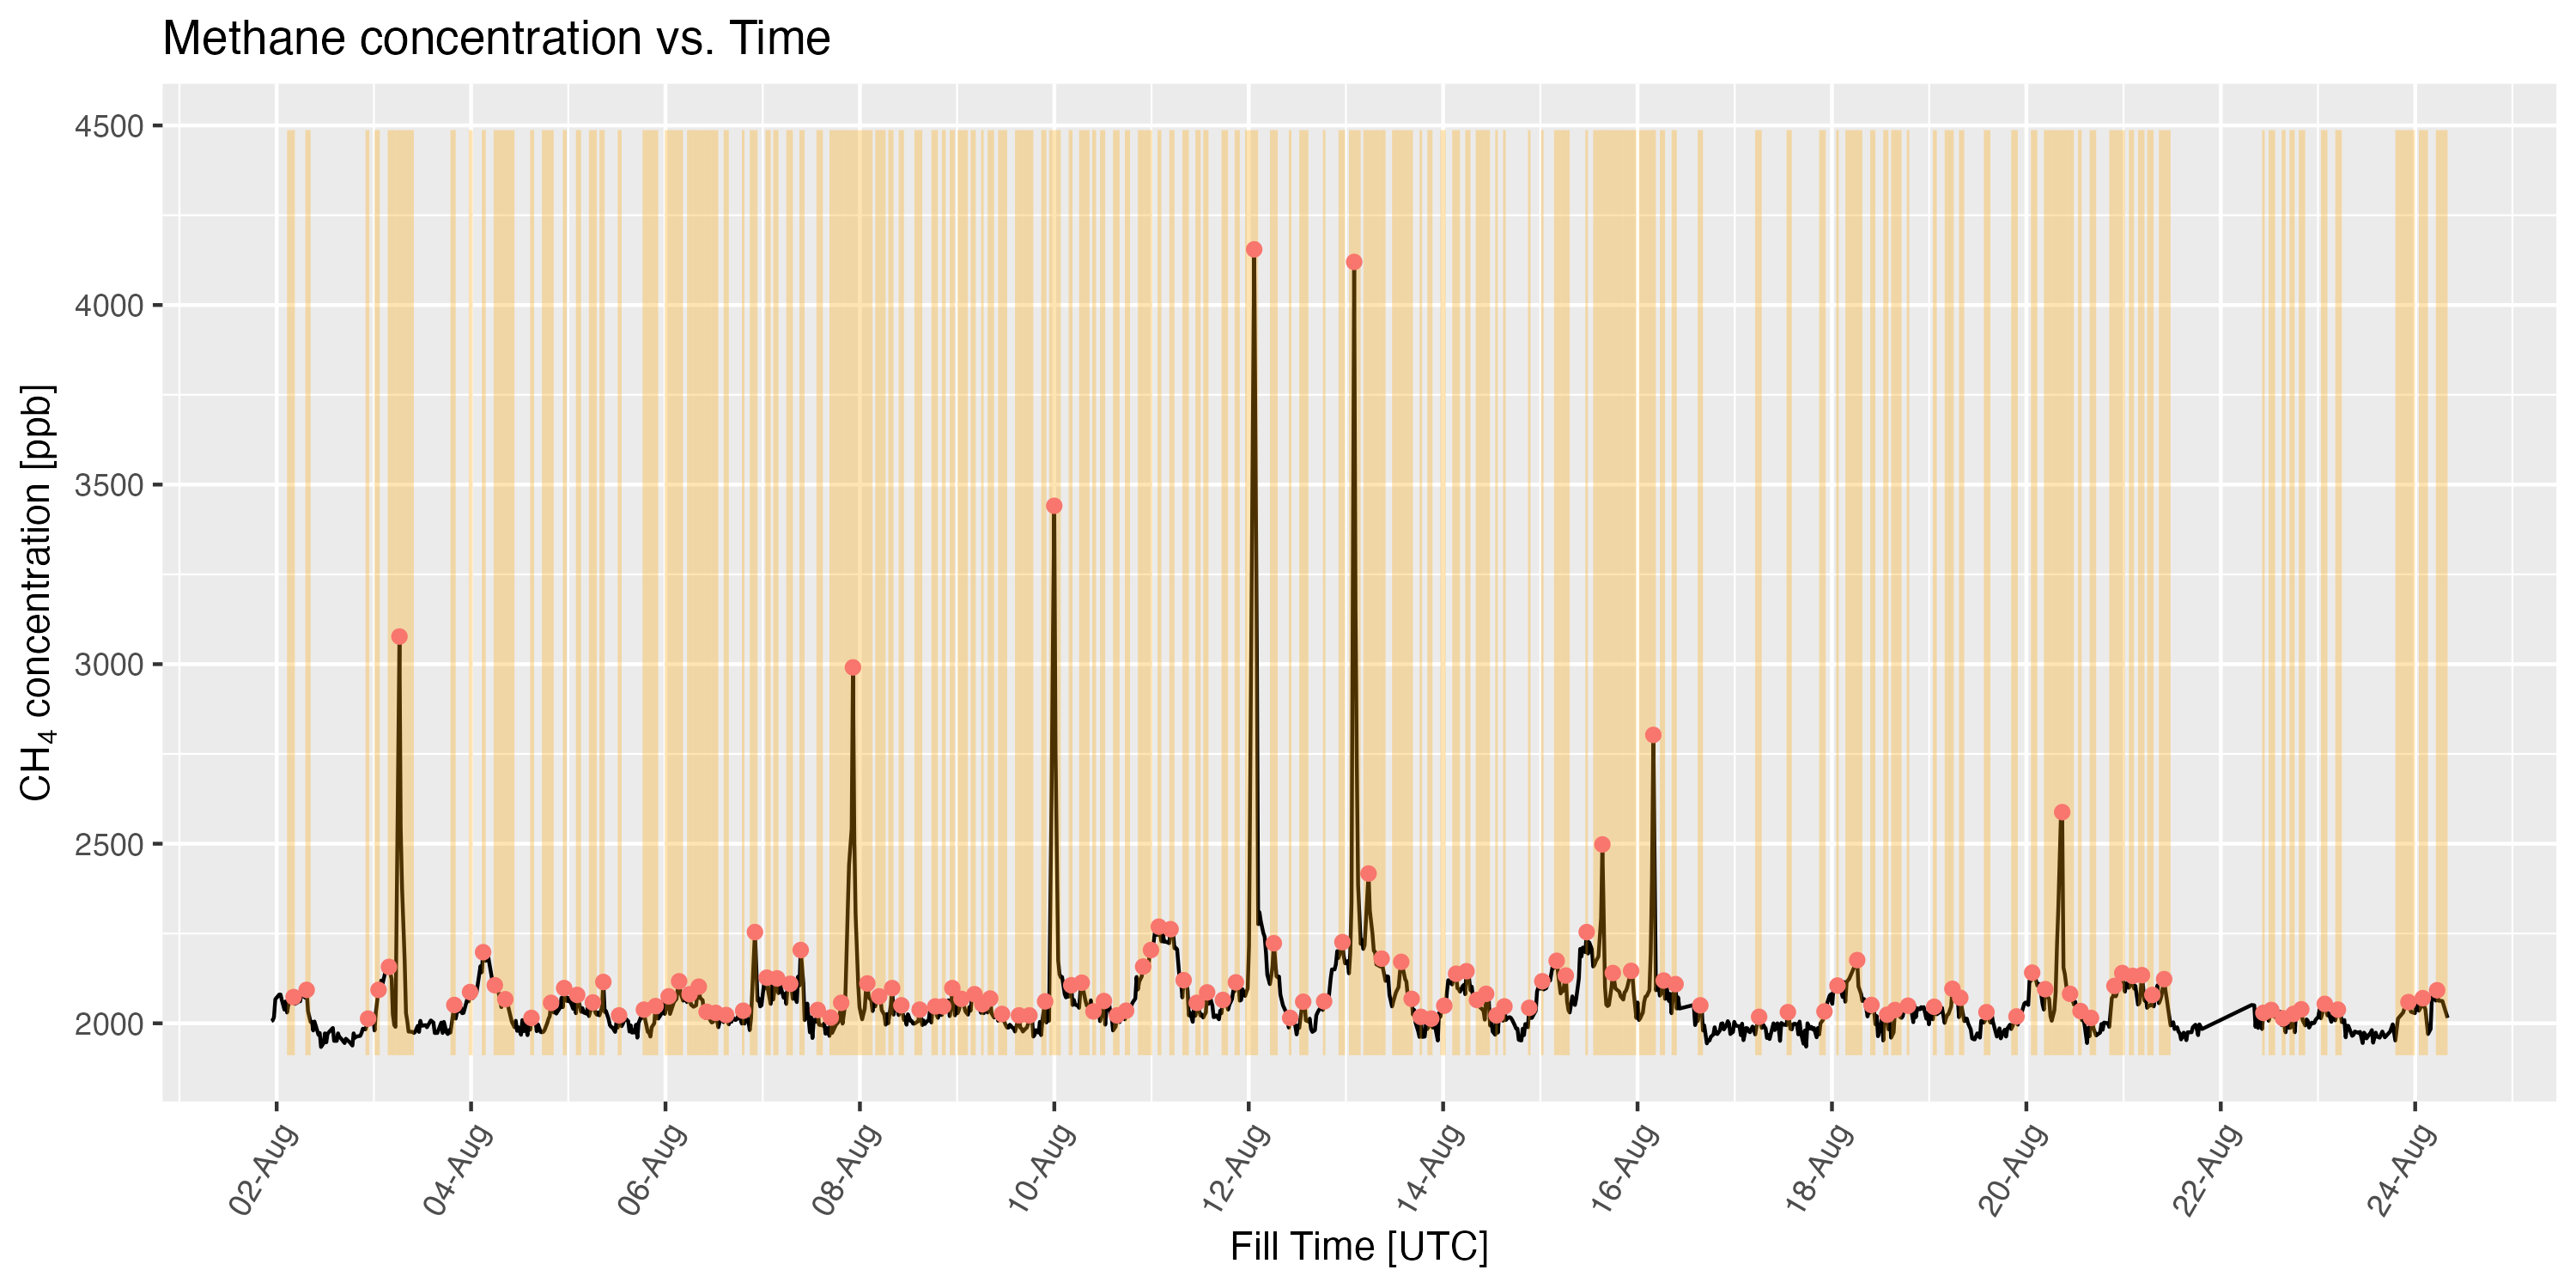
\includegraphics[width=1\textwidth]{figures/Appendix/CH4_Timelines/4_CH4_Timeline0_Paper_Peaks.png}
 \caption[CH$_4$ Timeline with peak identification from literature]{Section of CF-IRMS measurement showing the timeline of methane concentrations measured in Hamburg Geomatikum (83m above ground) from 02.08.2021 to 24.08.2021. Peak identification criteria by \cite{Menoud.2021}. The red dot indicates the peak centre and the orange section highlights the peak width.}
 \label{TimelinePeaksPaper}
\end{figure}
\begin{figure}[htbp]
 \centering
 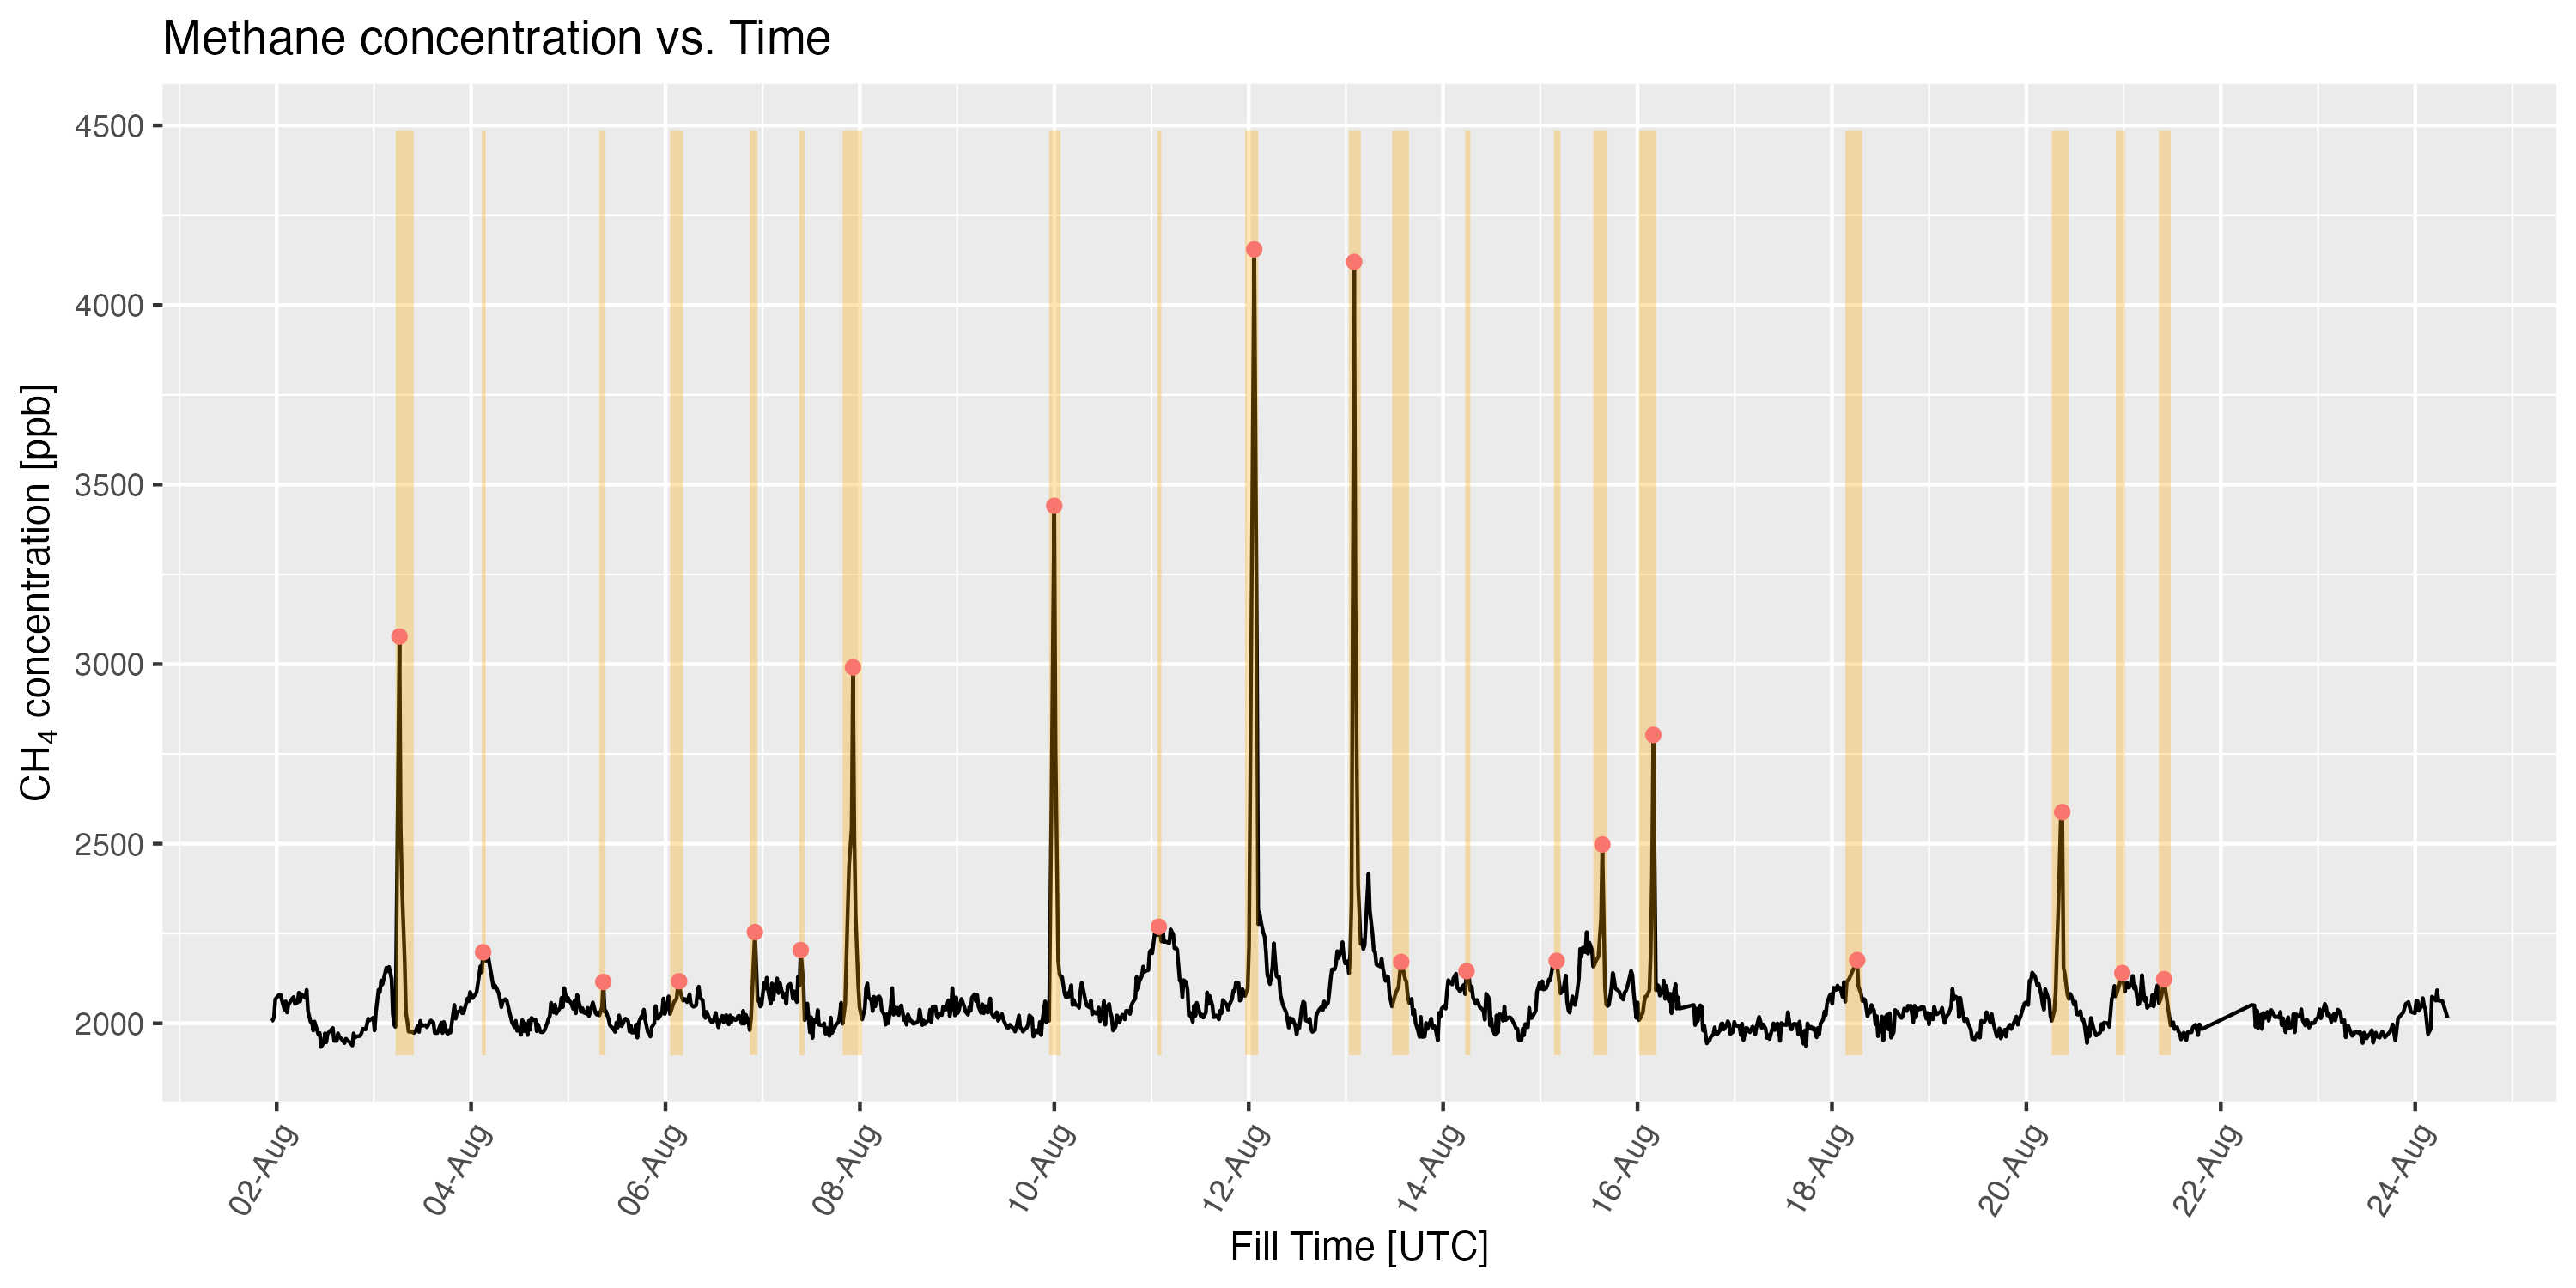
\includegraphics[width=1\textwidth]{figures/Appendix/CH4_Timelines/4_CH4_Timeline0_Medium_Peaks.png}
 \caption[CH$_4$ Timeline with strict peak identification]{Section of CF-IRMS measurements showing the timeline of methane concentrations measured in Hamburg Geomatikum (83m above ground) from 02.08.2021 to 24.08.2021. Peak identification criteria are chosen for only prominent peaks. The red dot indicates the peak centre and the orange section highlights the peak width.}
 \label{TimelineMediumPeaks}
\end{figure}
Nearly all peaks are accounted for in the first image, where the peaks are selected according to literature criteria. The smaller peaks occur at a relatively high frequency with a substantial irregularity. The number of peaks per day varies between 5 to 15 peaks. While during warmer months, August, September and October, the frequency of the peaks is lower than for the colder month, December, January, and February, see \cref{PeakHistogramm}.
\begin{table}[h!]
\centering
\begin{tabular}{||c c c c c c c c c||} 
 \hline
 & Aug. & Sep. & Oct. & Nov. & Dec. & Jan. & Feb. & Mar. \\ [0.5ex] 
 \hline\hline
  A: & 164 & 182 & 195 & 185 & 205 & 174 & 145 & 190 \\
  B: & 23 & 31 & 37 & 32 & 36 & 28 & 20 & 23 \\ [1ex] 
 \hline
\end{tabular}
\caption[Methane peaks per moth table]{Table of methane peaks per month using two different identification criteria. A: Selection criteria by \cite{Menoud.2021}. B: Strict criteria only selecting prominent peaks}
\label{PeakHistogramm}
\end{table}
Intermediate and prominent peaks occur at relatively regular intervals, while there are never more than two peaks within a day, and their peak centres are never closer than 12 h apart. \\
In the second image, the identification criteria are purposely designed to identify the prominent large and intermediate peaks and highlight the peaks well. Those peaks occur during the entire measurement campaign but with a higher frequency and concentration during the warmer months than the colder ones. The peaks are all quite sharp, i.e., with a short duration and high concentration compared to the background.

\section{Methane correlation analysis}
\subsection{Elbe water level methane correlation} \label{MethaneWaterLevel}
When the methane concentration timeline is overlayed with the water level of the Elbe, see \cref{TimelineCH4Waterlevel}, it can be seen that the prominent methane peak occurs shortly after the low water of the river. This behaviour is observed throughout the measurement period. The peaks occur, on average, 2$\pm$1 h after the low water.
\begin{figure}[htbp]
 \centering
 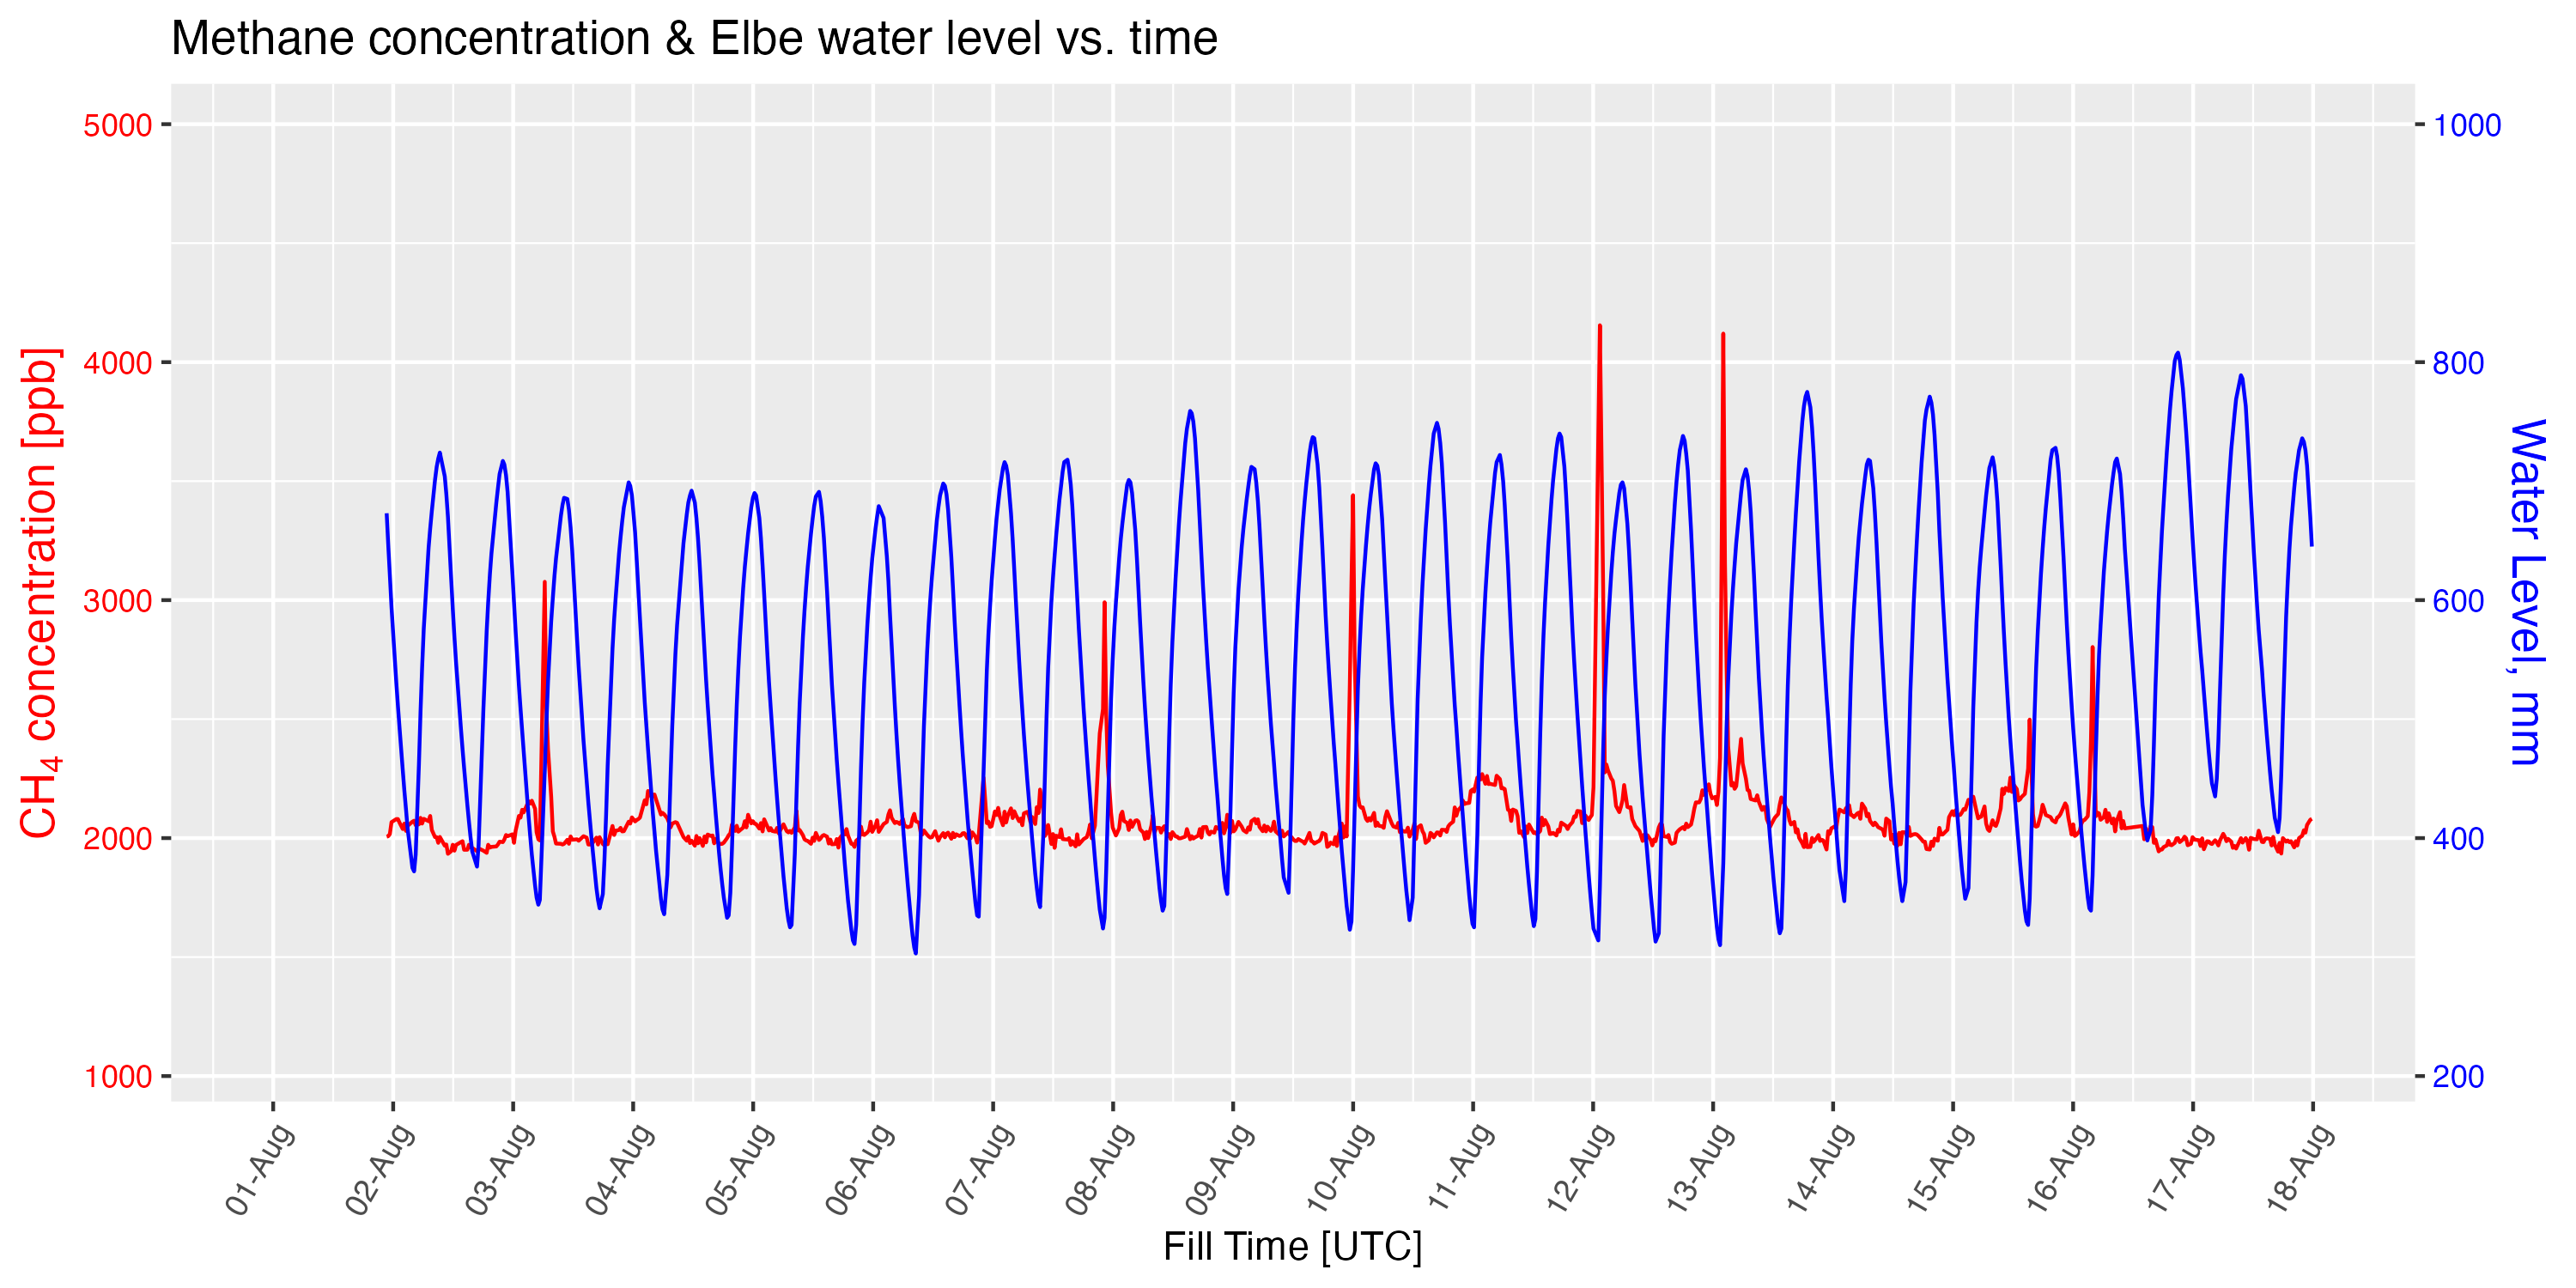
\includegraphics[width=1\textwidth]{figures/Appendix/Water_Level/1_CH4_WL.png}
 \caption[CH$_4$ Timeline with Elbe Water level Overlay]{Section of the CH$_4$ concentration timeline measured with the CF-IRMS at the Geomatikum (Red). Overlayed by the water level timeline of the river Elbe (blue). Measurements from 02.08.2021 to 18.08.2021 are shown.}
 \label{TimelineCH4Waterlevel}
\end{figure}
As the prominent methane peaks can’t be observed during every low water cycle of the river, additional factors seem to contribute to their production. But to establish a statistically meaningful correlation, Pearson's correlation coefficient between the water level and the methane concentration was investigated as previously described.
This correlation can be seen in  \cref{WaterLevelPCCGeomatikum}. Here, the measurements are binned by speed and direction using the Wind measurements made at the Geomatikum.
\begin{figure}
\centering
\begin{subfigure}[b]{1\textwidth}
   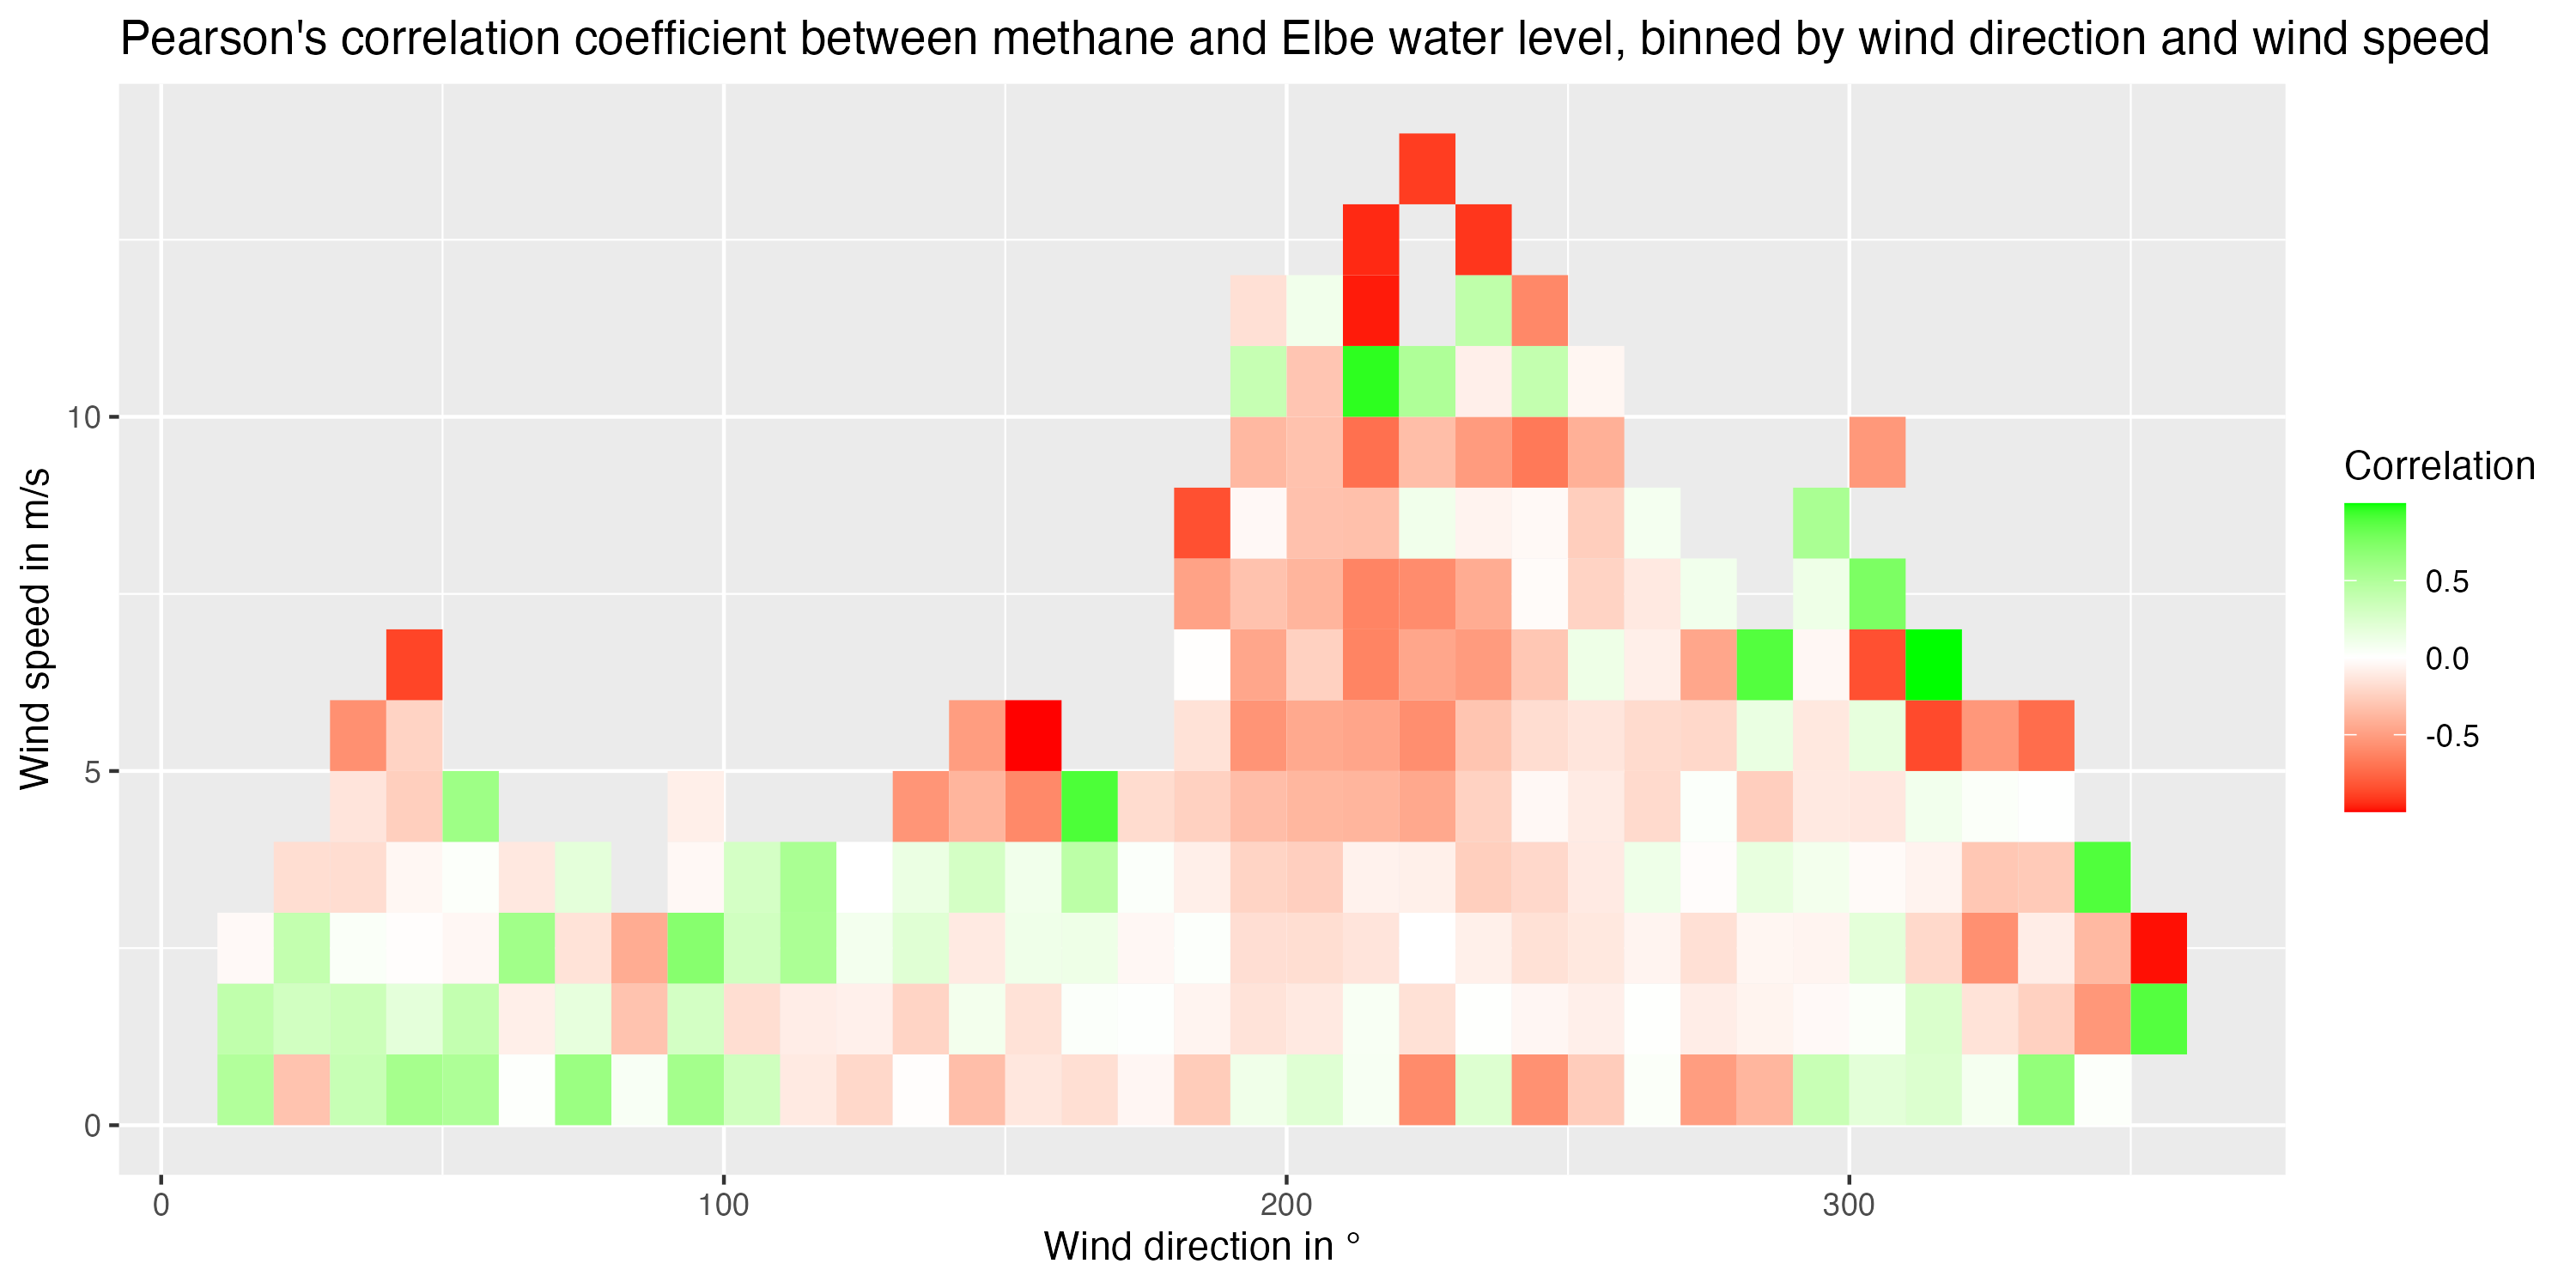
\includegraphics[width=1\linewidth]{figures/Appendix/Water_Level/13_CH4_vs_Waterlevel_Correlation_Geomatikum.png}
   \caption{}
   \label{WaterLevelPCCGeomatikum} 
\end{subfigure}
\begin{subfigure}[b]{1\textwidth}
   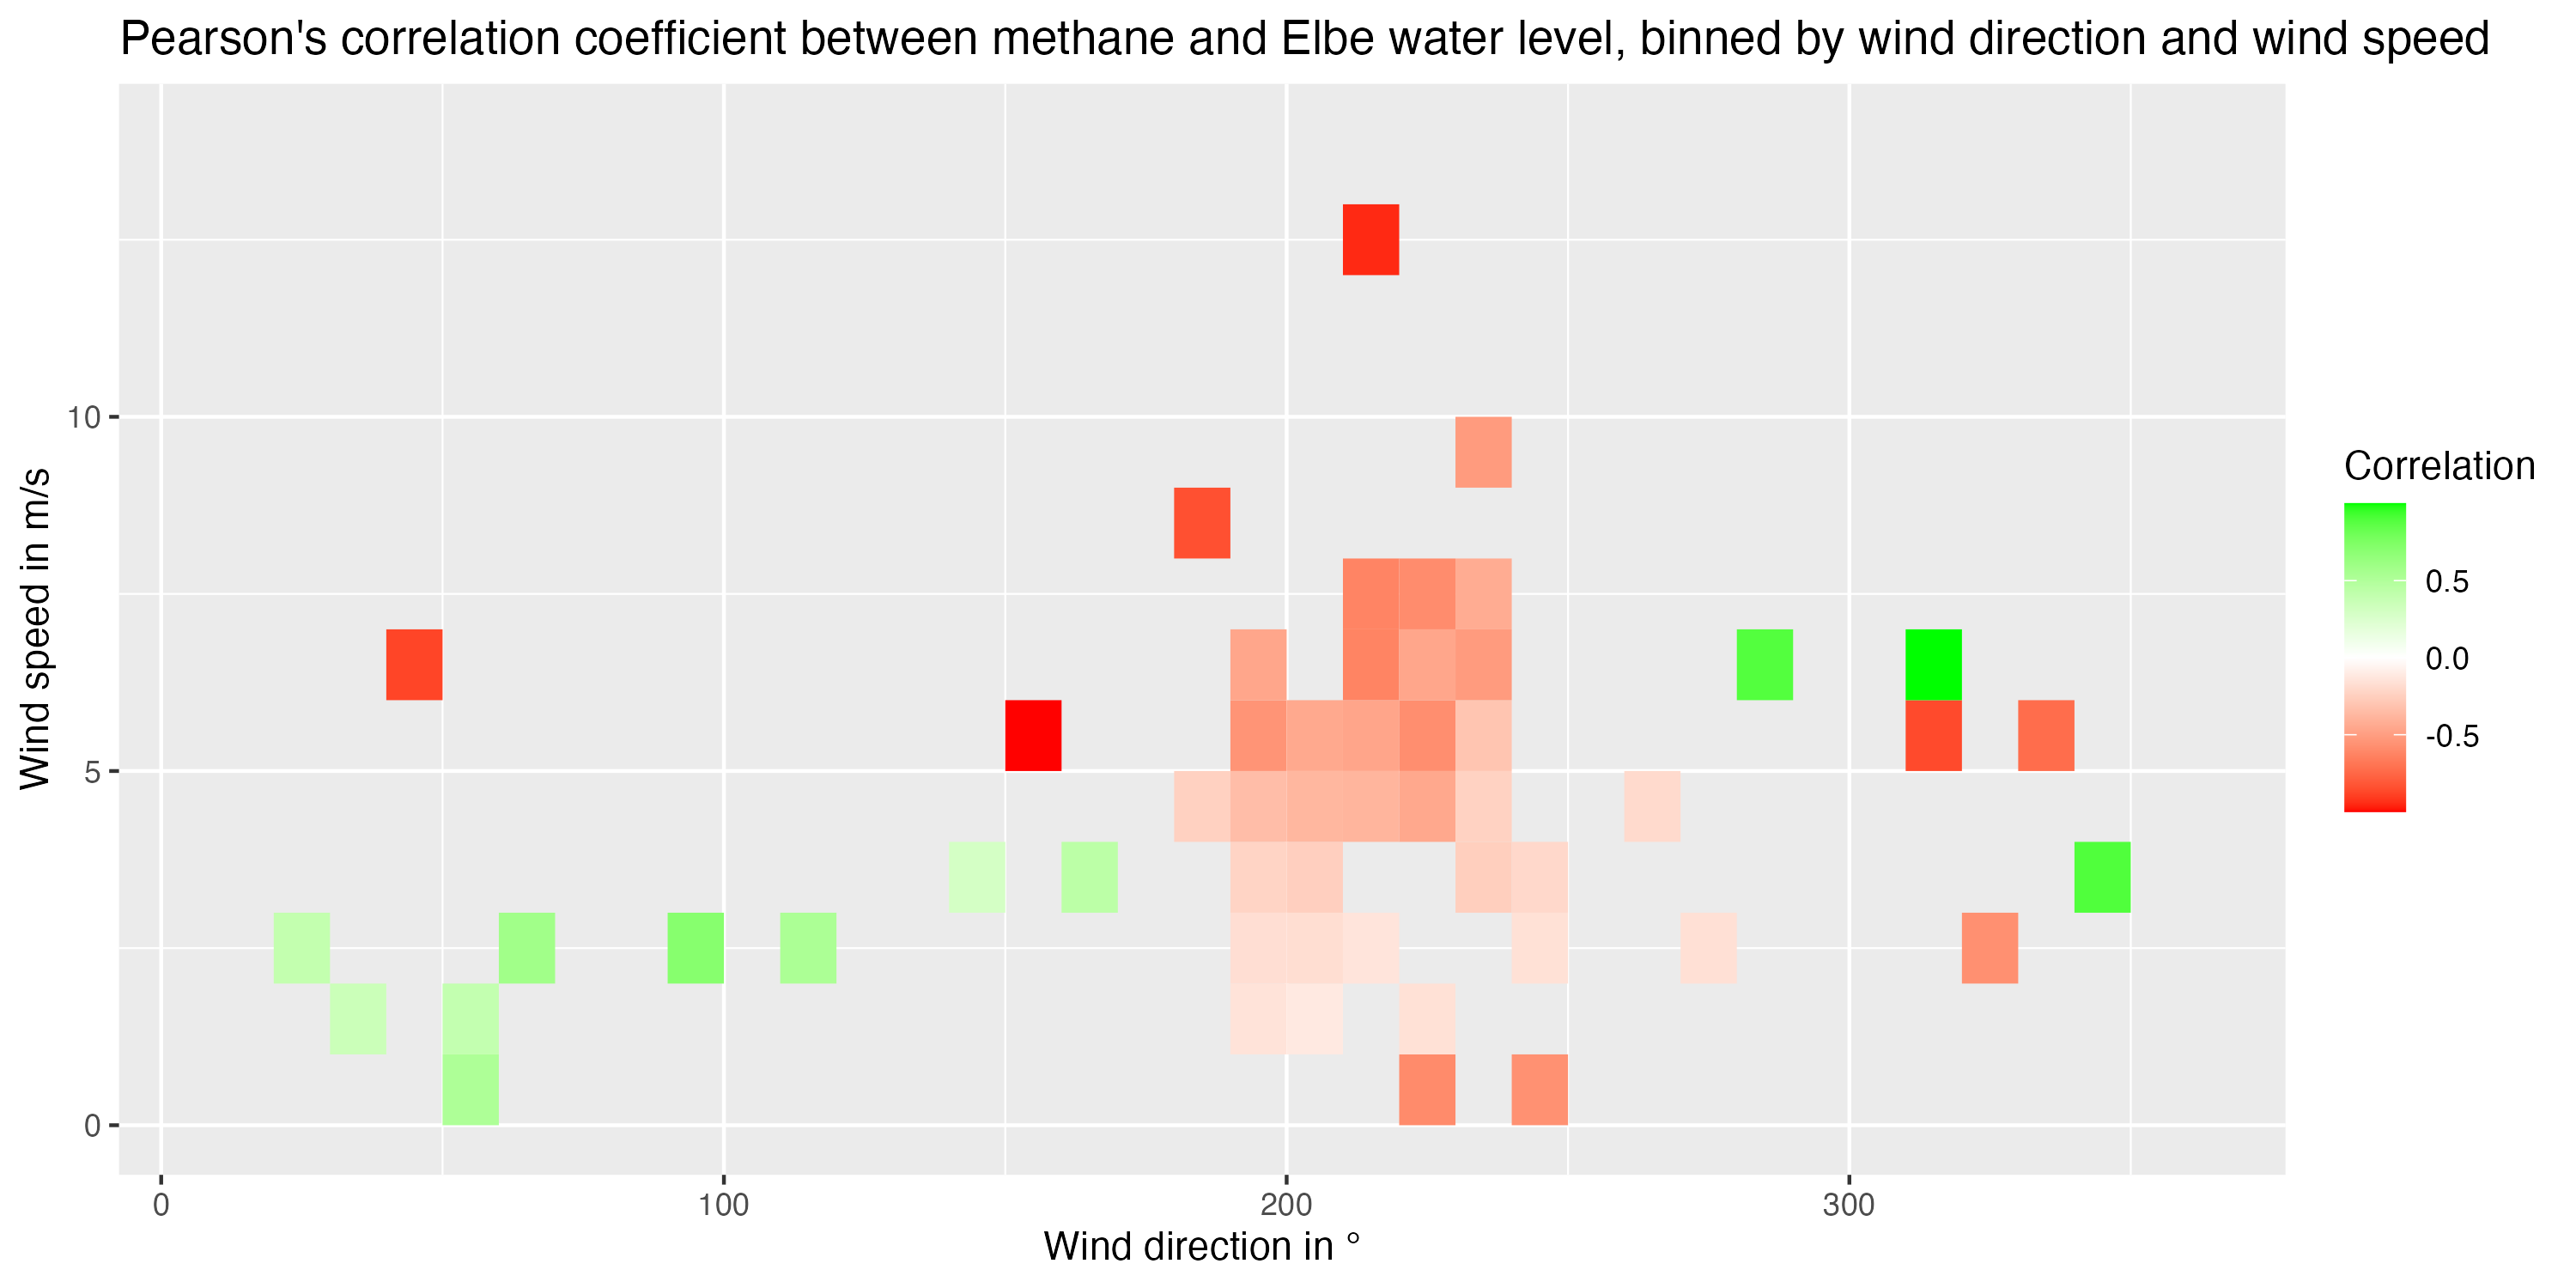
\includegraphics[width=1\linewidth]{figures/Appendix/Water_Level/13_CH4_vs_Waterlevel_Correlation_P_value_Geomatikum.png}
   \caption{}
   \label{WaterLevelCorrPValueGeomatikum}
\end{subfigure}
\caption[Correlation between CH$_4$ and Water level]{(a) Pearson's correlation coefficient between methane and Elbe water level, binned by wind direction and wind speed. Green shows a positive correlation (enhanced CH$_4$ at high water level), and Red shows a negative correlation (enhanced CH$_4$ at low water level). (b) Shows only the correlations which pass the 5\% P-value test for methane and Elbe water level, binned by wind direction and wind speed.}
\label{WaterLevelCorrelationGeomatikum}
\end{figure}
The plot shows a positive correlation with a green colour and a negative correlation with a red colour. A positive correlation indicates an elevated methane concentration in the air with a high water level of the Elbe. In contrast, a negative correlation indicates a correlation between methane concentration in the air with a low water level of the Elbe. The P-value test in \cref{WaterLevelCorrPValueGeomatikum} checks if the correlation is statistically meaningful. If the P-value is $<$0.05 it passes the test and is indicated as such in the plot.\\
The correlation plot \cref{WaterLevelCorrPValueGeomatikum} shows a negative correlation that  passes the p-value test at a wind direction 180° and 250° with a wind speed of 1 m/s and 7 m/s.  \\
Following the direction of the wind leads to the port region of Hamburg, where the water height measurement was performed by Wasserstraßen- und Schifffahrtsverwaltung des Bundes (WSV) at Hamburg St. Pauli.\\
%add reference!!!!!!!!!!!
The remaining wind bins that include the wind directions East, North and West don't show reliable correlations between the water level and the methane concentration measured at the Geomatikum.  From the Geomatikum to its East, North and West, significantly fewer  water bodies are free-flowingly connected to the Elbe are present. Those waterbodies don’t experience the tidal effects.\\
The overall methane concentration and presence of peaks are generally higher when the Elbe experiences lower overall water levels. And Visa versa, fewer methane peaks and a lower concentration are observed at high water periods. The variation in the water levels for extended amount of time is due to changes in meteorological influences over an annual cycle and the lunar cycle influences in the tide. This can be seen in \cref{TimelineCH4WaterlevelRollingAverage} showing a plot of the total measurement campaign with a rolling average of one month for the water level and the methane concentration measured at the Geomatikum.
\begin{figure}[htbp]
 \centering
 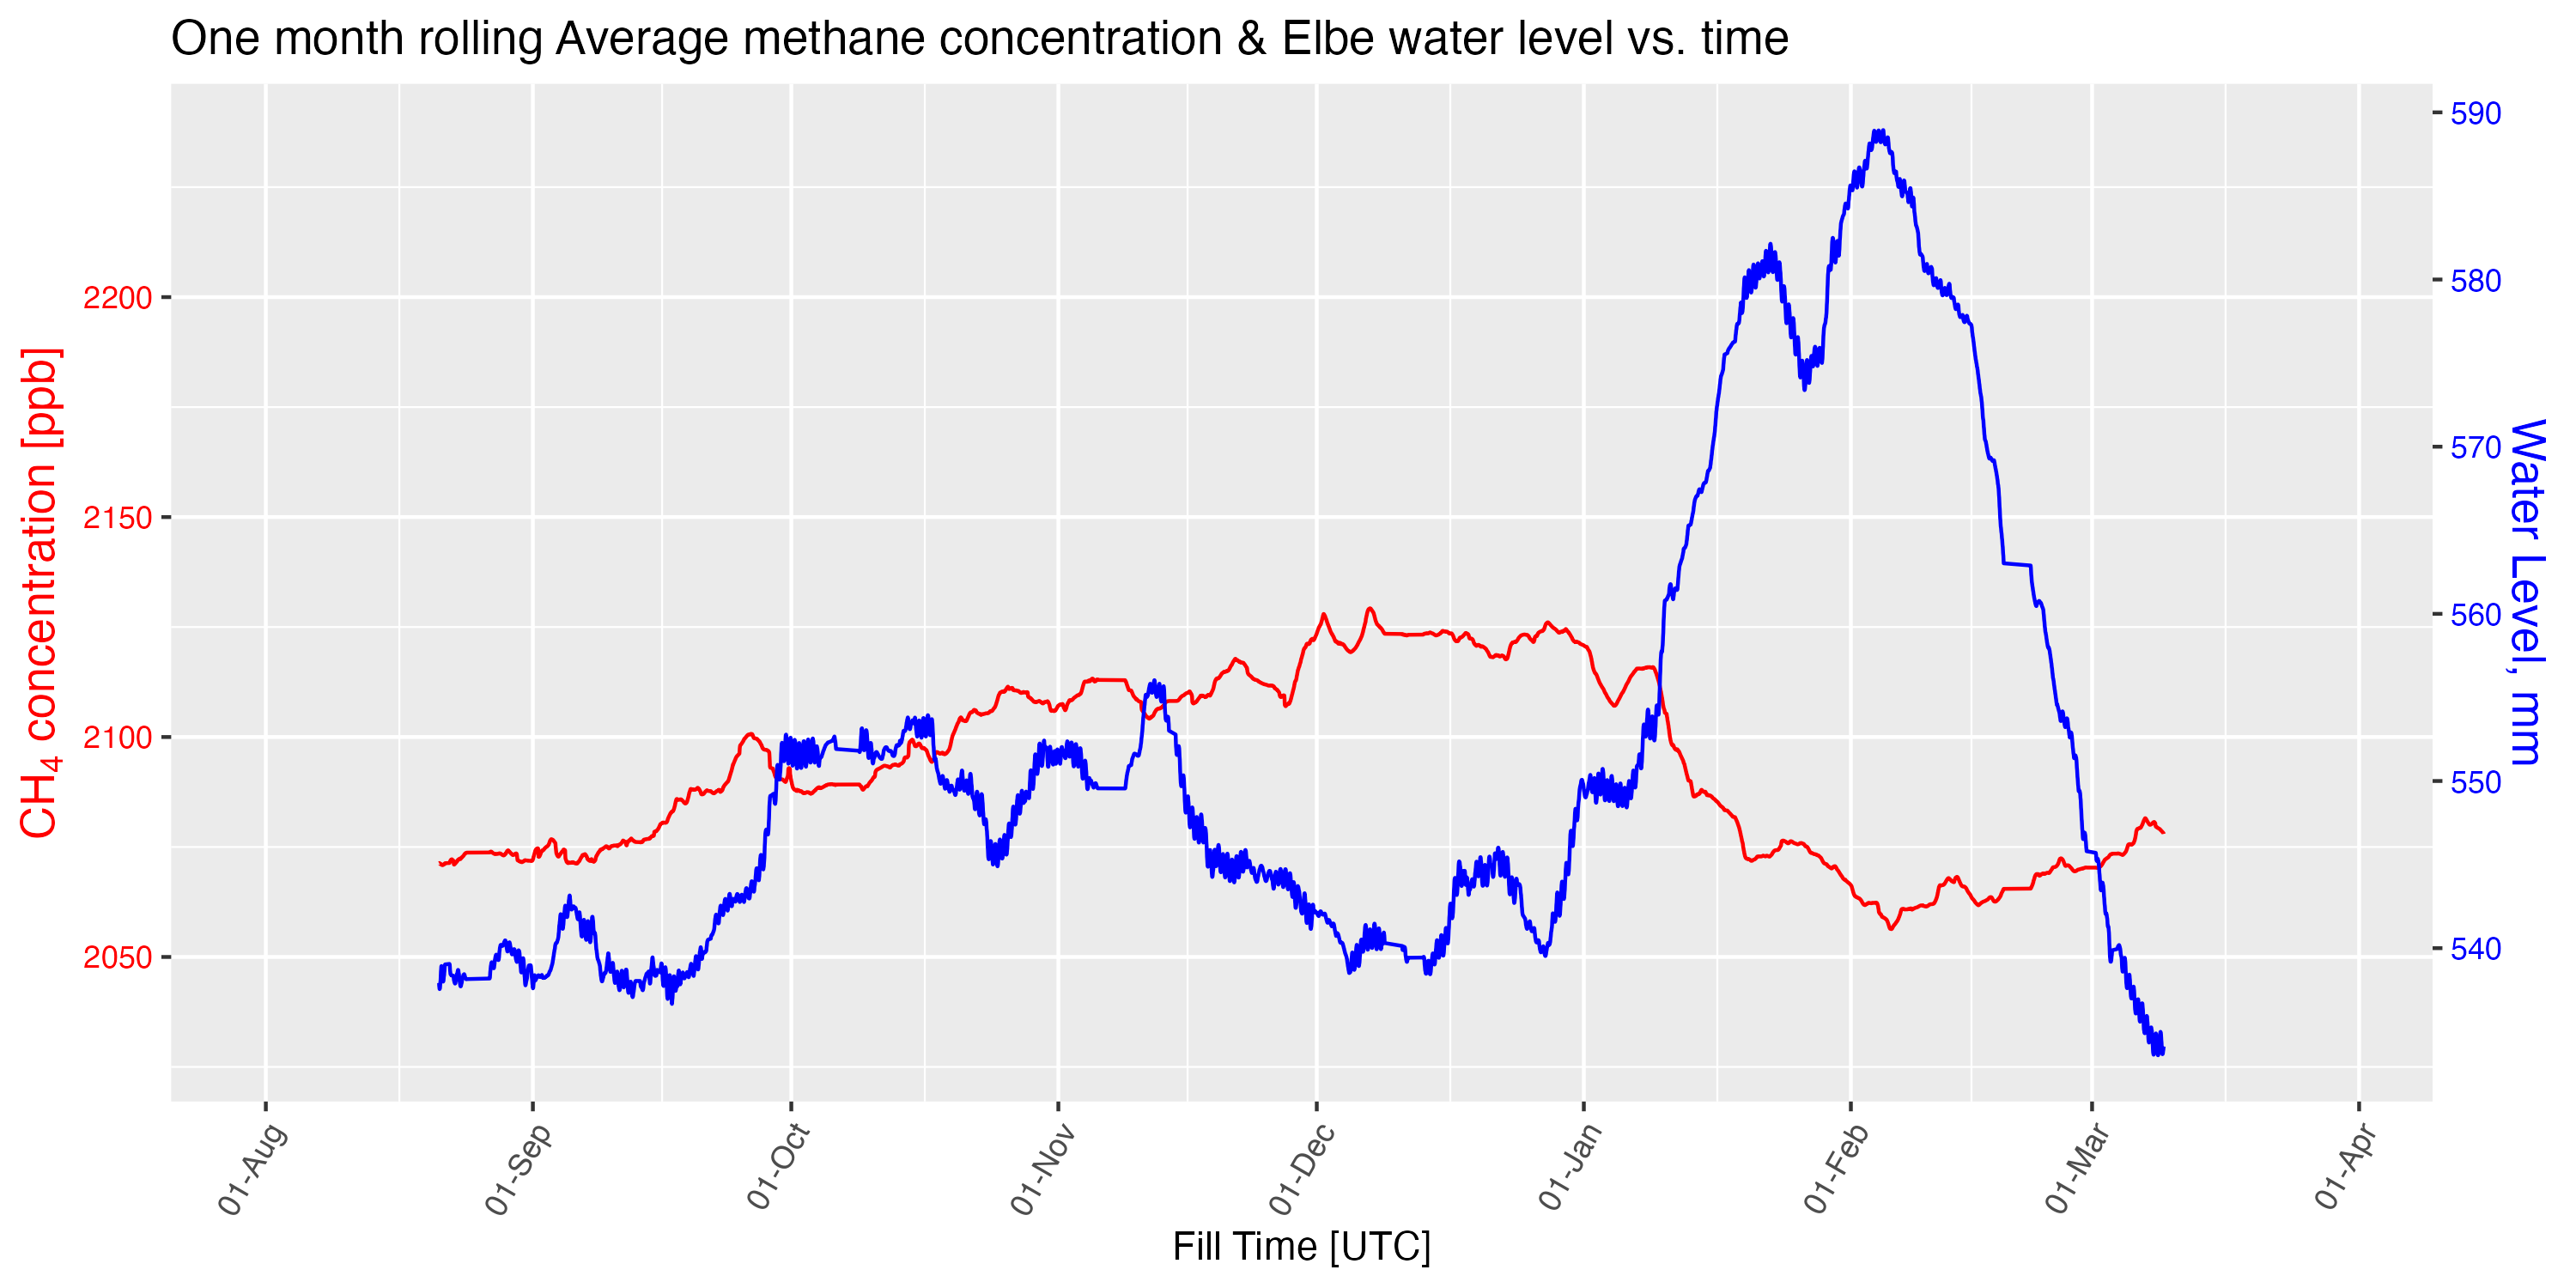
\includegraphics[width=1\textwidth]{figures/Appendix/Water_Level/1_CH4_WLRollingAverage.png}
 \caption[Rolling Average of one month CH$_4$ Timeline with Elbe Water level Overlay]{Rolling average timeline plot of CH$_4$ concentration measured with the CF-IRMS at the Geomatikum (Red) overlayed by the water level timeline of the river Elbe (blue).}
 \label{TimelineCH4WaterlevelRollingAverage}
\end{figure}
While a perfect linear correlation between the water level and the methane concentration was not observed when not regarding  the wind direction and speed. The correlations that were observed, for particular wind directions and speeds, indicate that a significant amount of methane measured at the Geomatikum originates from the Elbe that also correlates to its tidal movements.

\subsection{Elbe water quality methane correlation}
The water quality parameters measured at Elbe Seemannshöft provided by Hamburg Service were used \cite{IHUW.20230501} and were also investigated using Pearson's correlation coefficient and the P-value test. The influence of the Elbe can be seen in a particular region of wind direction and wind speeds in the resulting binned correlation plots \cref{CorrelationWaterQuality}. This region is around 180° to 300° for a wind speed between 1.5 m/s to 7 m/s. And are highlighted by blue circles in the plots. In this general direction from the Geomatikum, the river is located and is most drastically influenced by the tides. Further to the east, a series of locks block the tide in the river, while to the west, the Elbe is significantly wider and more naturalised. \cite{Matousu.2019} has shown a 10 times lower methane concentration in the Elbe in this section.\\
Apart from the water level of the Elbe discussed previously, some water quality parameters also show a good correlation with the methane concentration in the air measured a the Geomatikum.\\
Those include the water temperature, oxygen concentration and saturation, turbidity, UV absorption and pH level. The water temperature is the only parameter that shows a positive correlation this the methane concentration measured at the Geomatikum. All other parameters show a negative correlation with the methane concentration. All previously listed parameters pass the P-value test in the blue highlighted region that represents the general direction of the Elbe.
\begin{figure*}[t!]
    \subfloat[Water Temperature]{%
        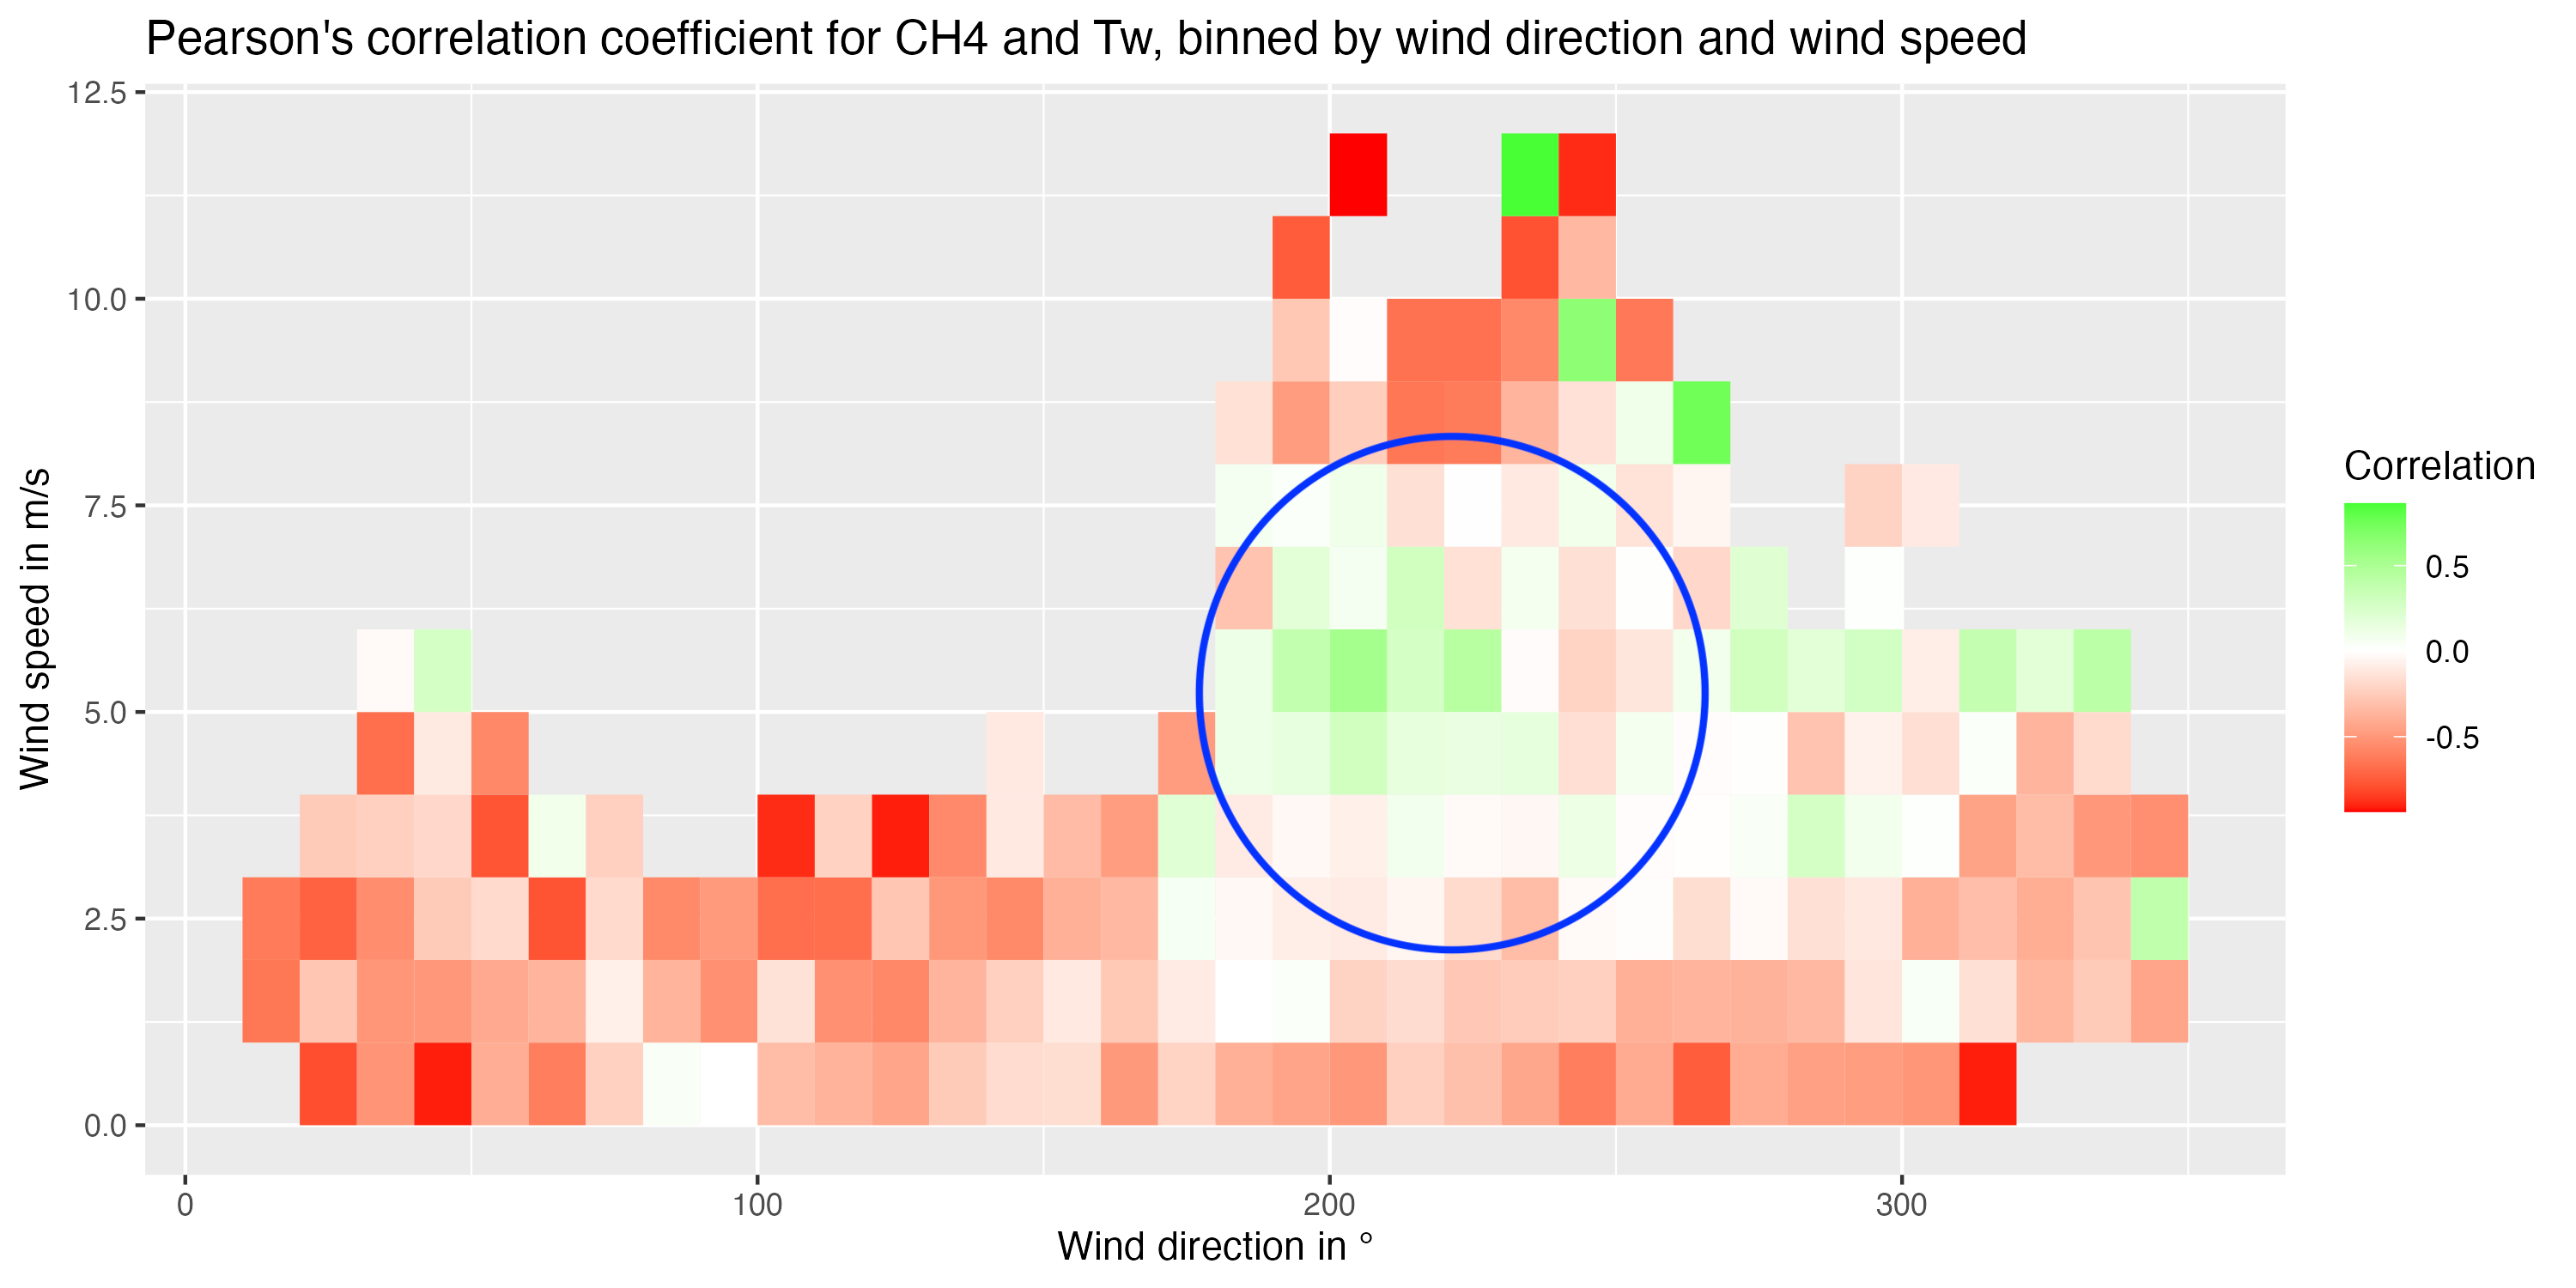
\includegraphics[width=.48\linewidth]{figures/Appendix/Water_Quality/13_CH4_vs_Water_Temp_Correlation_Geomatikum.png}%
        \label{CorrWaterTemp}%
    }\hfill
    \subfloat[O$_2$ concentration]{%
        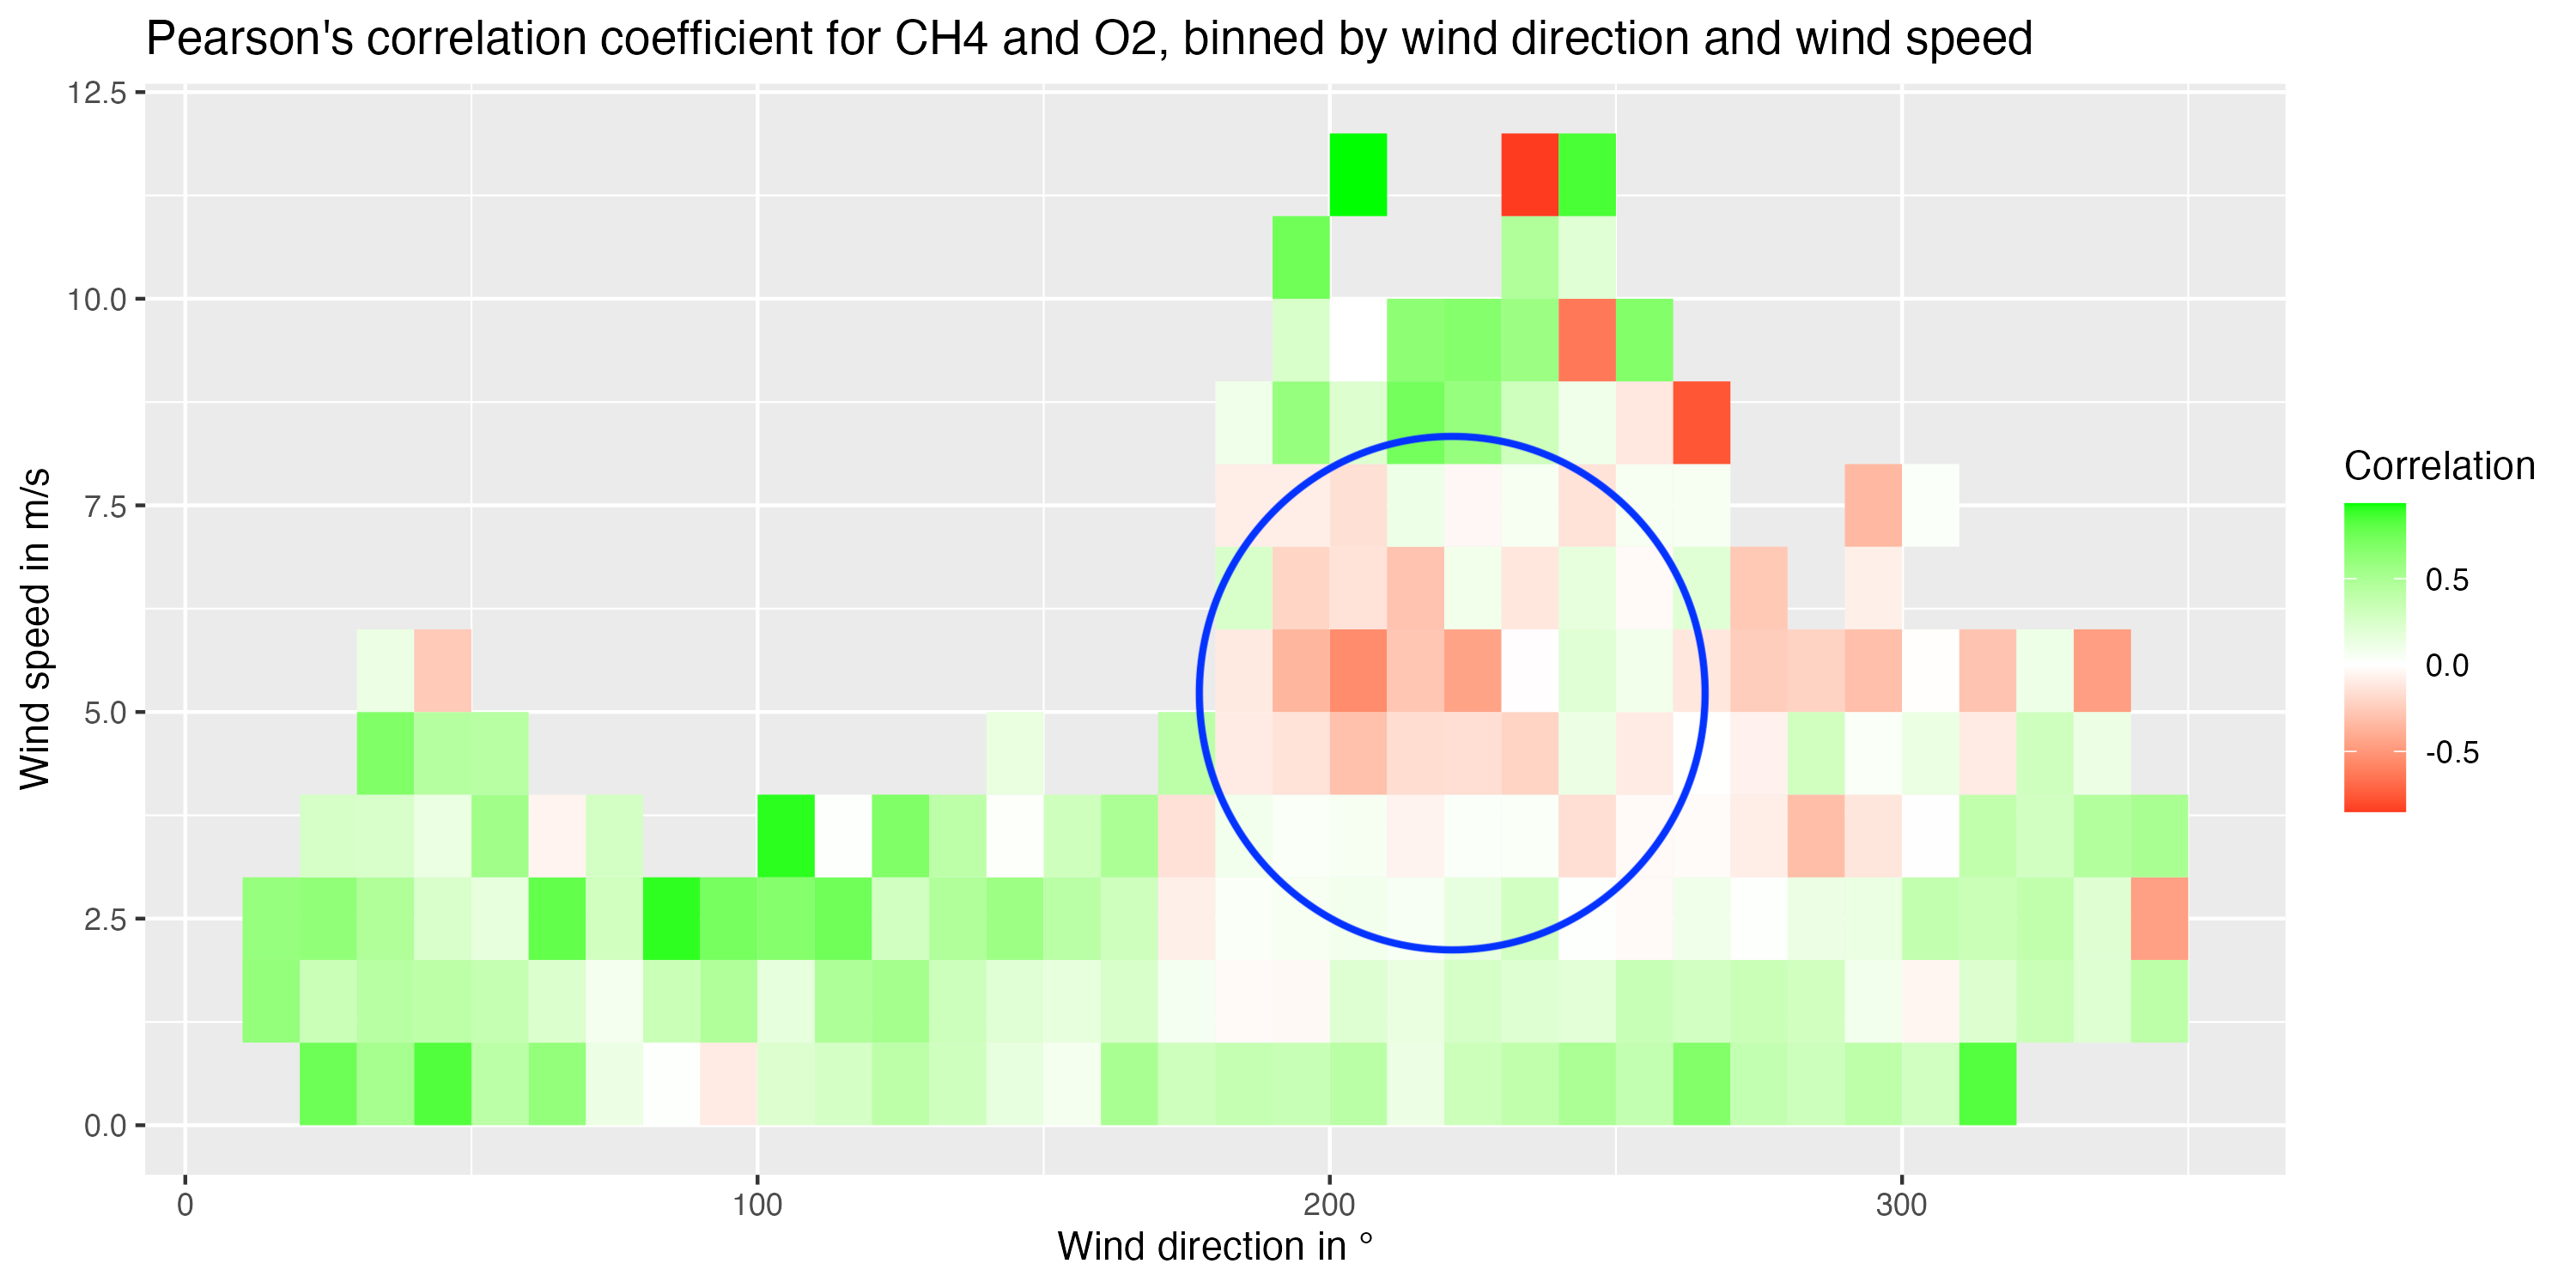
\includegraphics[width=.48\linewidth]{figures/Appendix/Water_Quality/13_CH4_vs_O2_Correlation_Geomatikum.png}%
        \label{CorrO2}%
    }\\
    \subfloat[pH-value]{%
        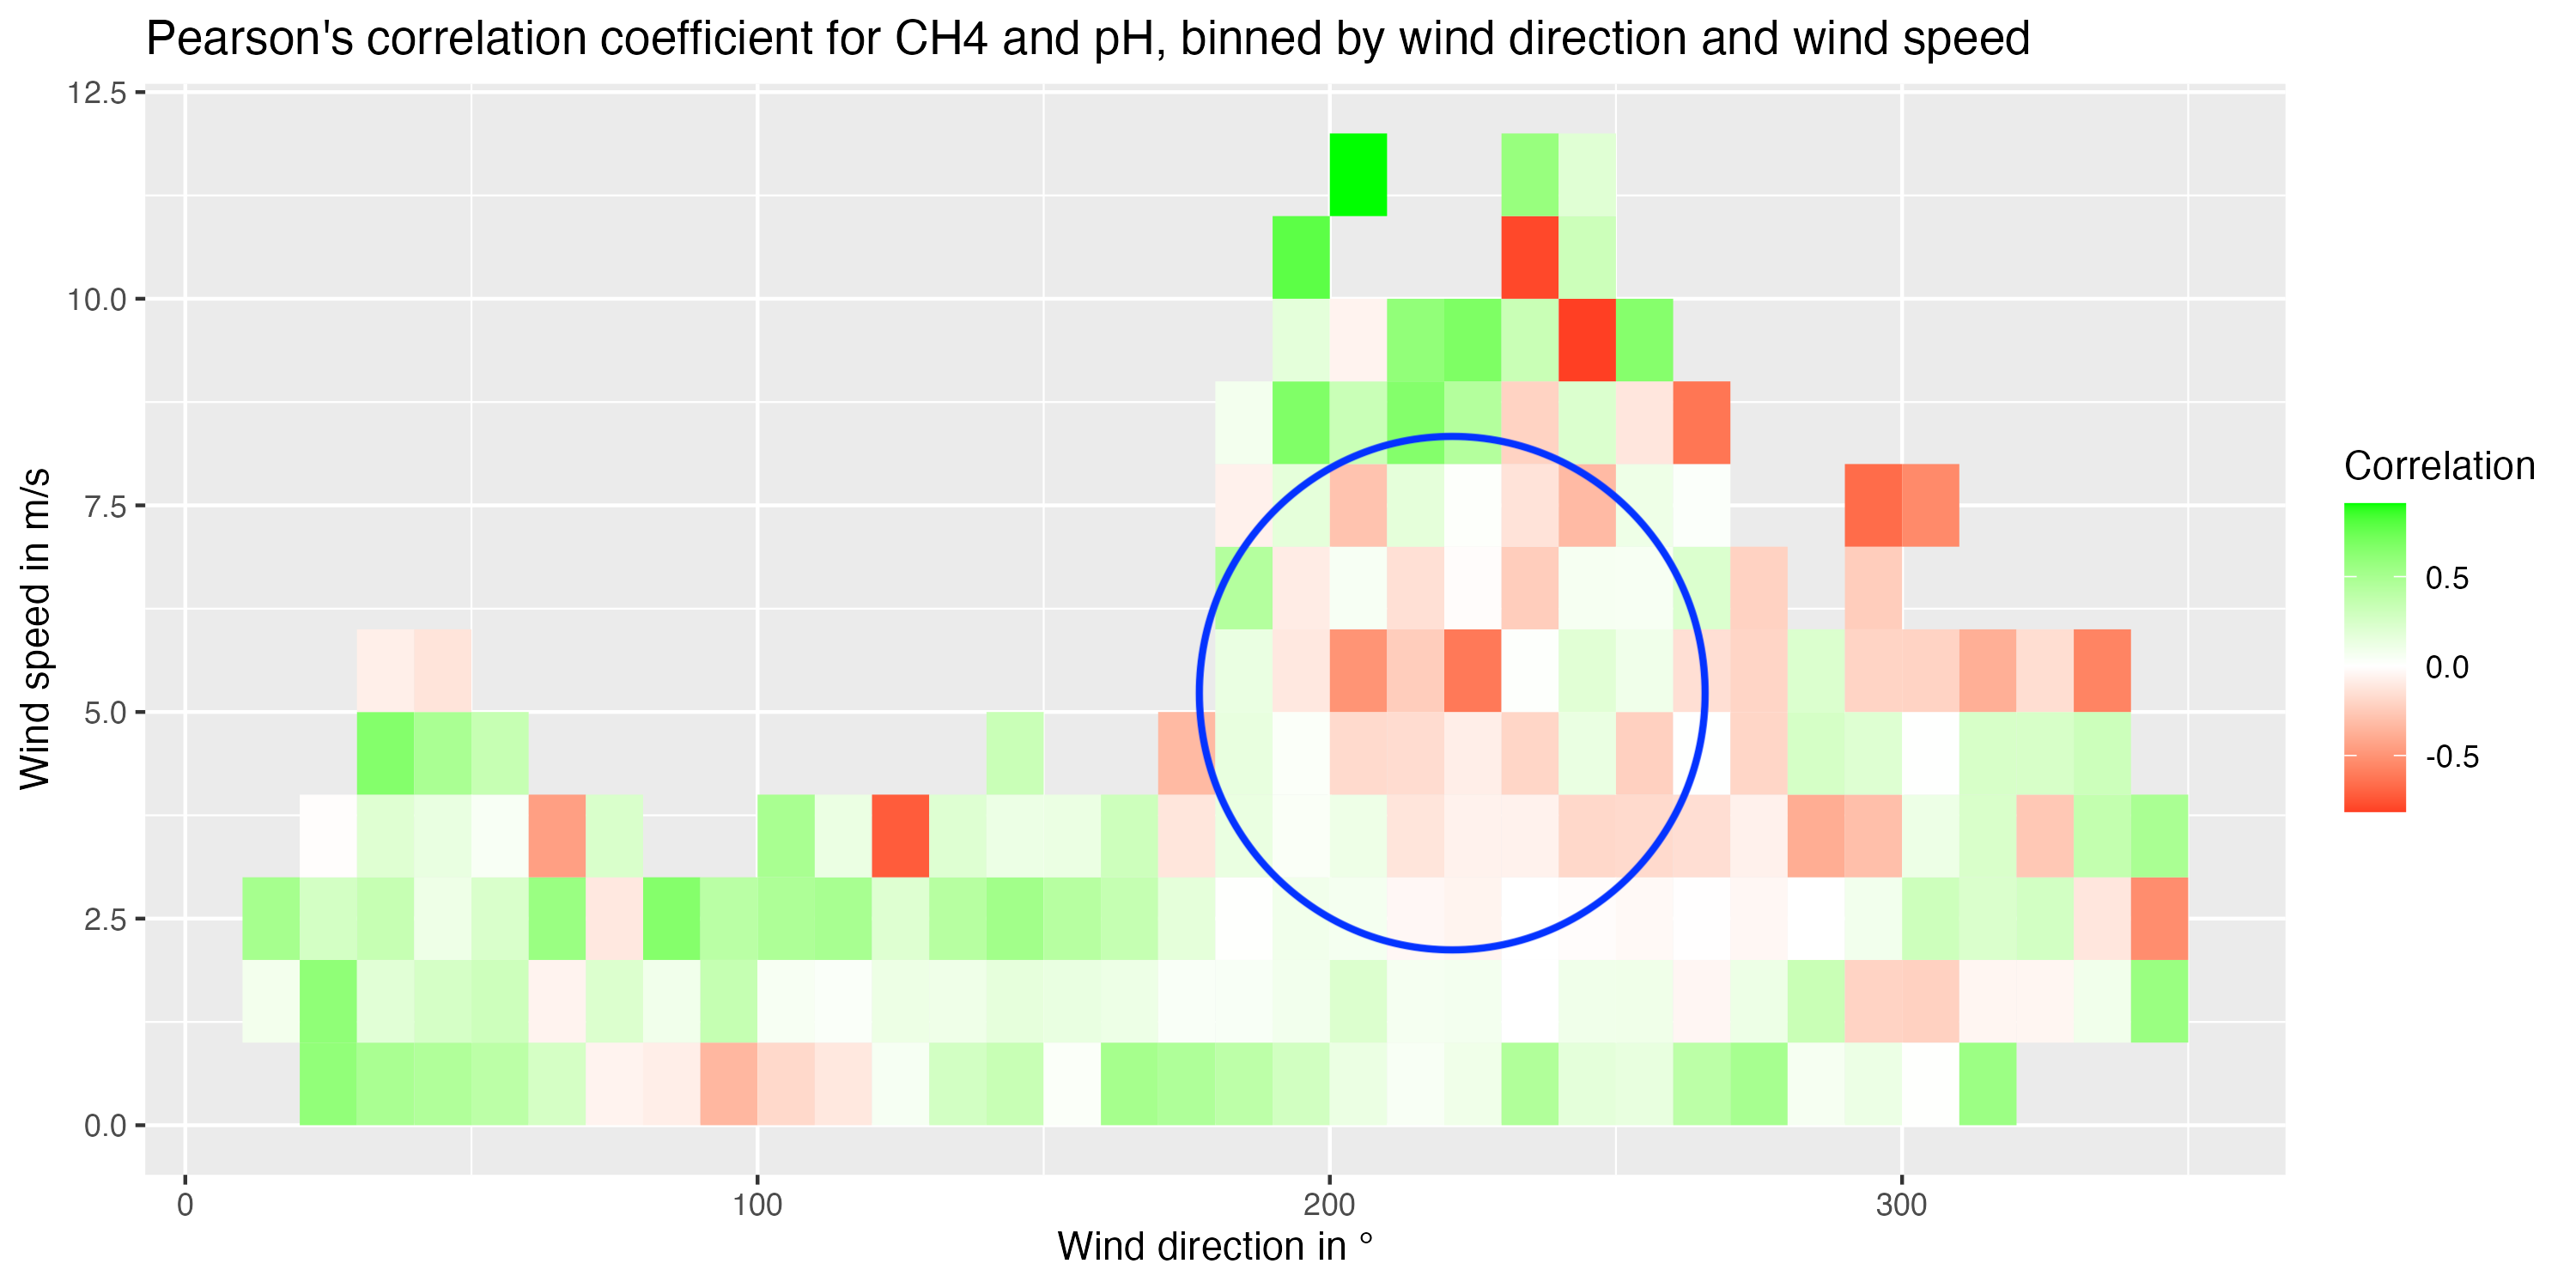
\includegraphics[width=.48\linewidth]{figures/Appendix/Water_Quality/13_CH4_vs_pH_Correlation_Geomatikum.png}%
        \label{CorrPH}%
    }\hfill
    \subfloat[Turbidity]{%
        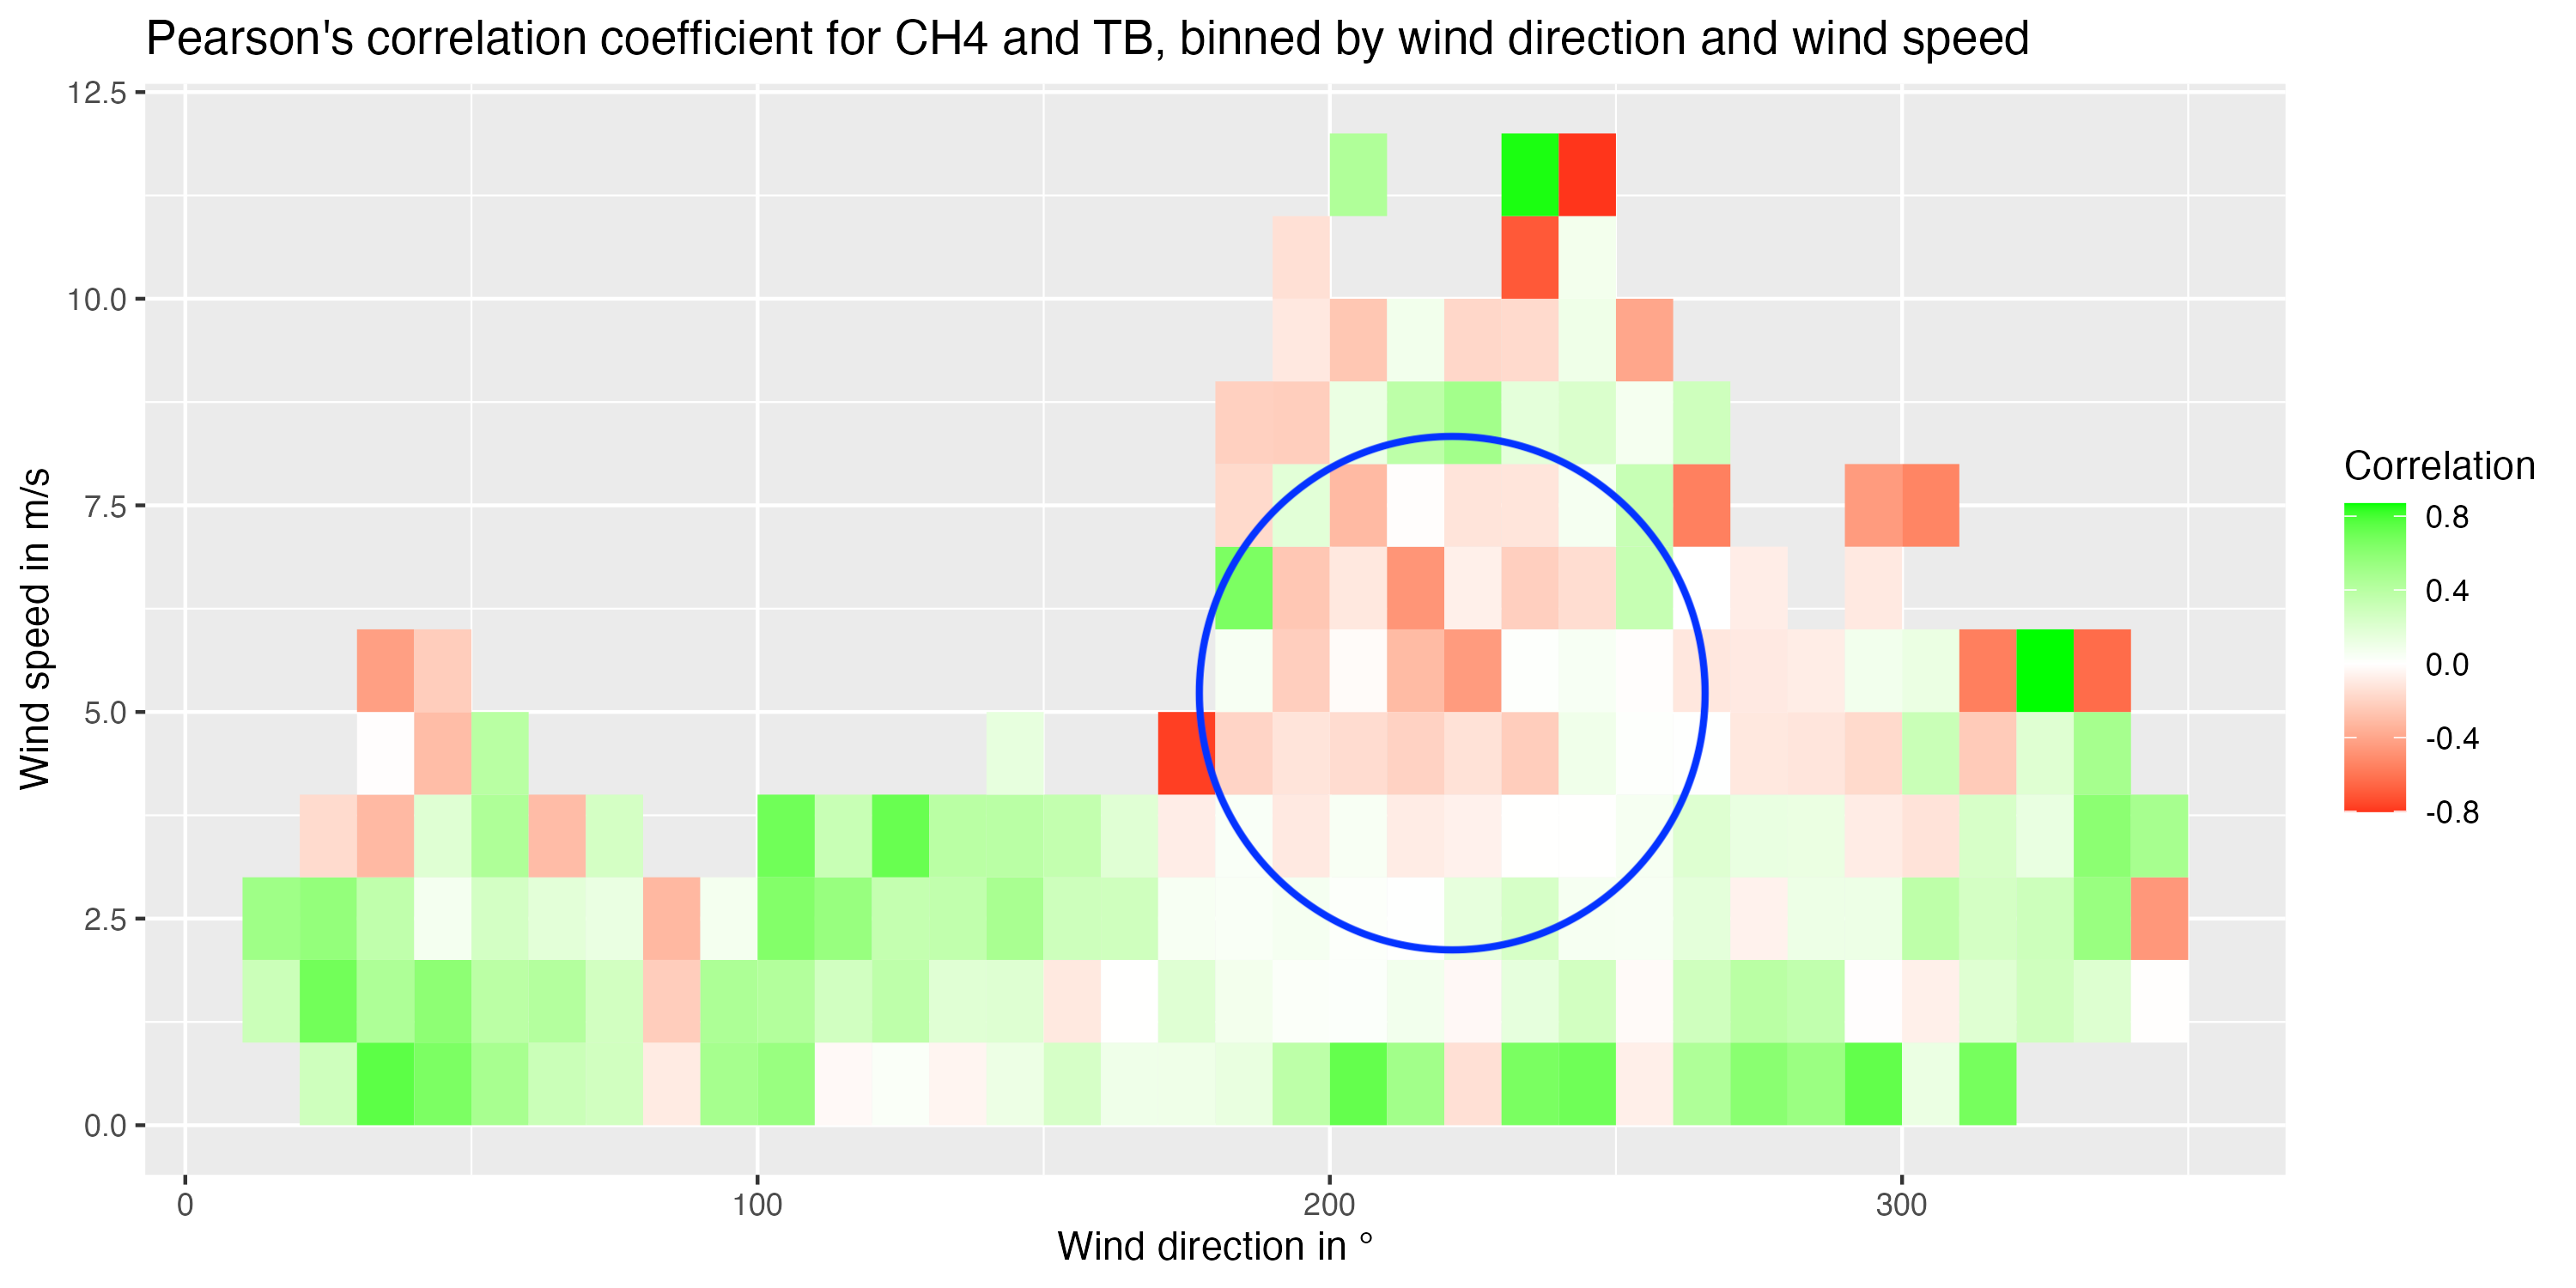
\includegraphics[width=.48\linewidth]{figures/Appendix/Water_Quality/13_CH4_vs_Turbidity_Correlation_Geomatikum.png}%
        \label{CorrTur}%
    }
    \caption[Correlation between CH$_4$ and Water quality]{Pearson's correlation coefficient between methane-air concentration and Elbe water quality parameters, binned by wind direction and wind speed. Green shows a positive correlation (enhanced CH$_4$ at high values), and Red shows a negative correlation (enhanced CH$_4$ at values). The blue circles indicate the wind direction and speed where the Elbe has a strong influence.}
    \label{CorrelationWaterQuality}
\end{figure*}
Other water quality parameters, such as electrical conductivity and algae concentrations (Chlorophyll concentration of various different species), don't show a correlation with the measured methane concentration. Those parameters don't seem to influence the microbial health in the Elbe significantly enough to influence their methane production and reduction mechanisms substantially.

\subsection{Meteorological observation and methane correlation}
%needs correction!!!!
The meteorological data measured by the DWD at Hamburg-Fuhlsbüttel \cite{DeutschenWetterdienst.20230501} was investigated in the same manner as the water parameters of the Elbe.
Pearson's correlation coefficient and P-value test for the meteorological parameter with the methane concentration in the air show some correlations between them. Those include air temperature, solar radiation, dewpoint and humidity.\\
The humidity and dewpoint measurements have a general correlation for all wind directions and speeds, excluding the region 180° - 300° and (0.5 to 3.5 m/s). In this region, no significant correlation can be observed. This can be seen in \cref{CorrHumid} and \cref{CorrDewPoint}, where the black circle indicates this region. Following these wind directions and considering the low wind speeds leads to the densely urbanised city centred, where very few natural areas such as parks and gardens are present.\\
The temperature and solar radiation correlate significantly with the methane concentration. A negative correlation is observed in nearly all regions, only excluding the 180° - 250° and (1.5 to 7 m/s) region. In this wind direction, the Elbe is located, and the methane emissions from the Elbe seem to dominate in this region. In figure \cref{CorrAirTemp} and \cref{CorrRadiation}, this region is indicated by blue circles.
The remaining region shows a significant negative correlation between the temperature and solar radiation with the methane concentration in the air. In particular, the wind directions from 330° to 130° show a very strong negative correlation at all wind speeds. The wind direction in this region point to the primarily residential regions of Hamburg. The Elbe is not present in this region, and no tidal-influenced waterbodies exist there. The Keeling plot analyses with regards to wind direction, which will be discussed later, indicated a strong anthropogenic methane production influence, such as fossil fuel combustion. This is also confirmed by \cite{Maazallahi.2020}, who found numerous gas infrastructure leakages and a generally high anthropogenic methane mixture in this region using street-level mobile measurements. 
\begin{figure*}[t!]
    \subfloat[Humidity]{%
        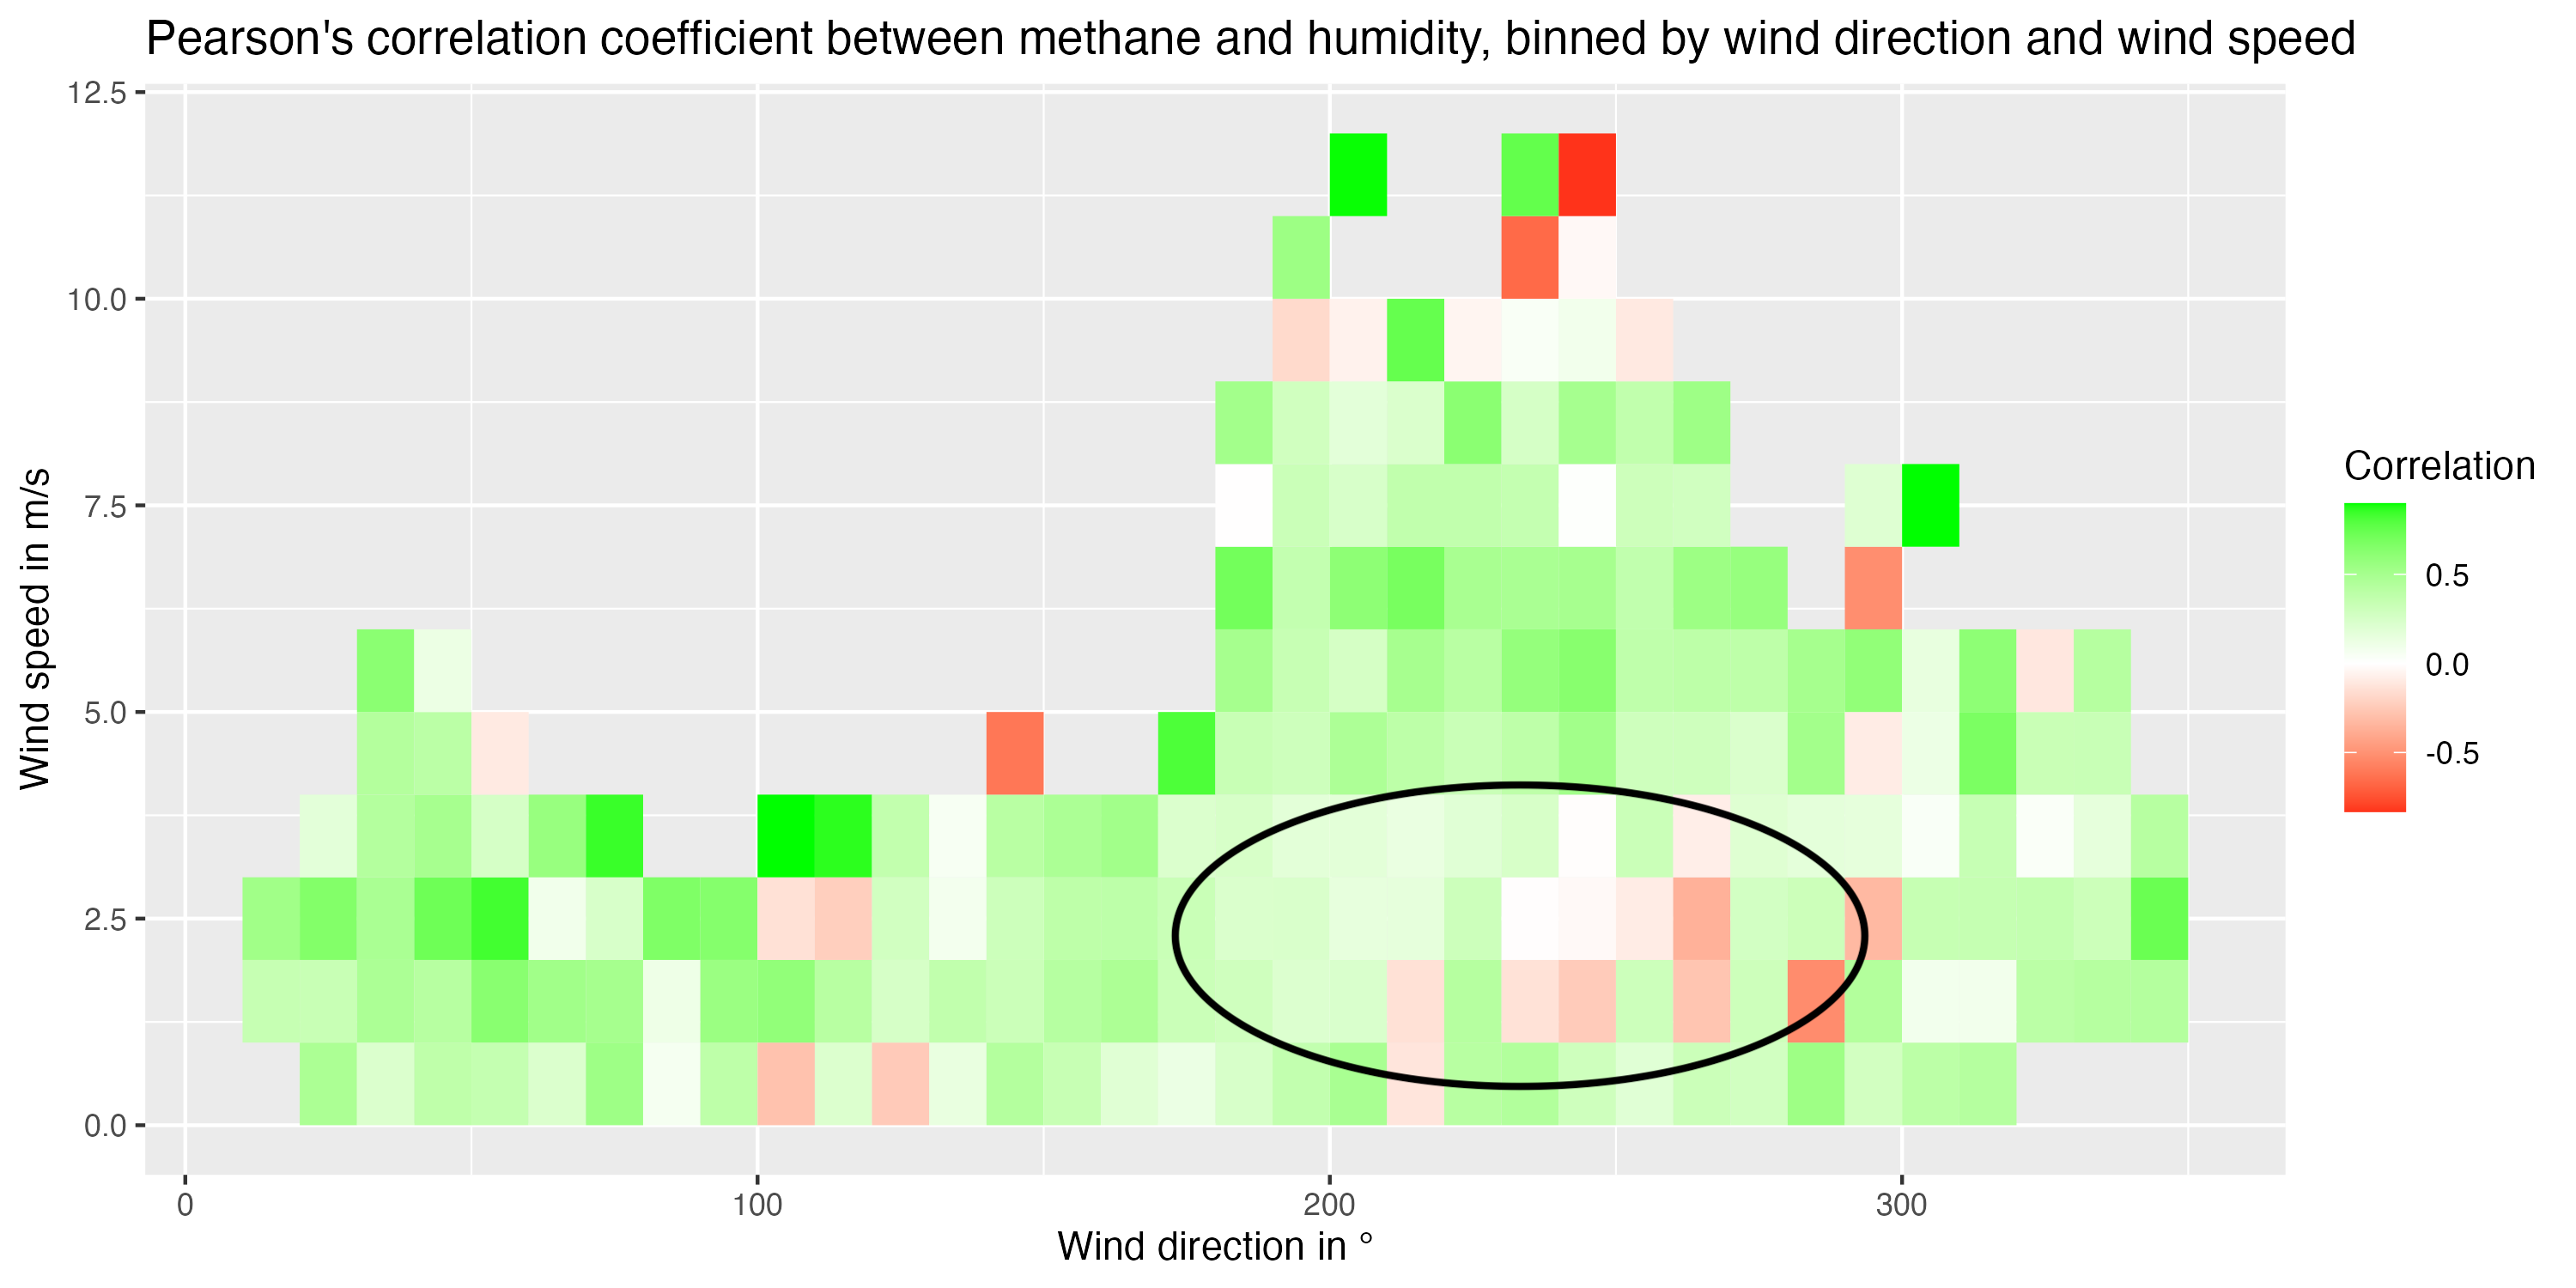
\includegraphics[width=.48\linewidth]{figures/Appendix/Meteorological/13_CH4_vs_humidity_Correlation_Geomatikum.png}%
        \label{CorrHumid}%
    }\hfill
    \subfloat[Dew point]{%
        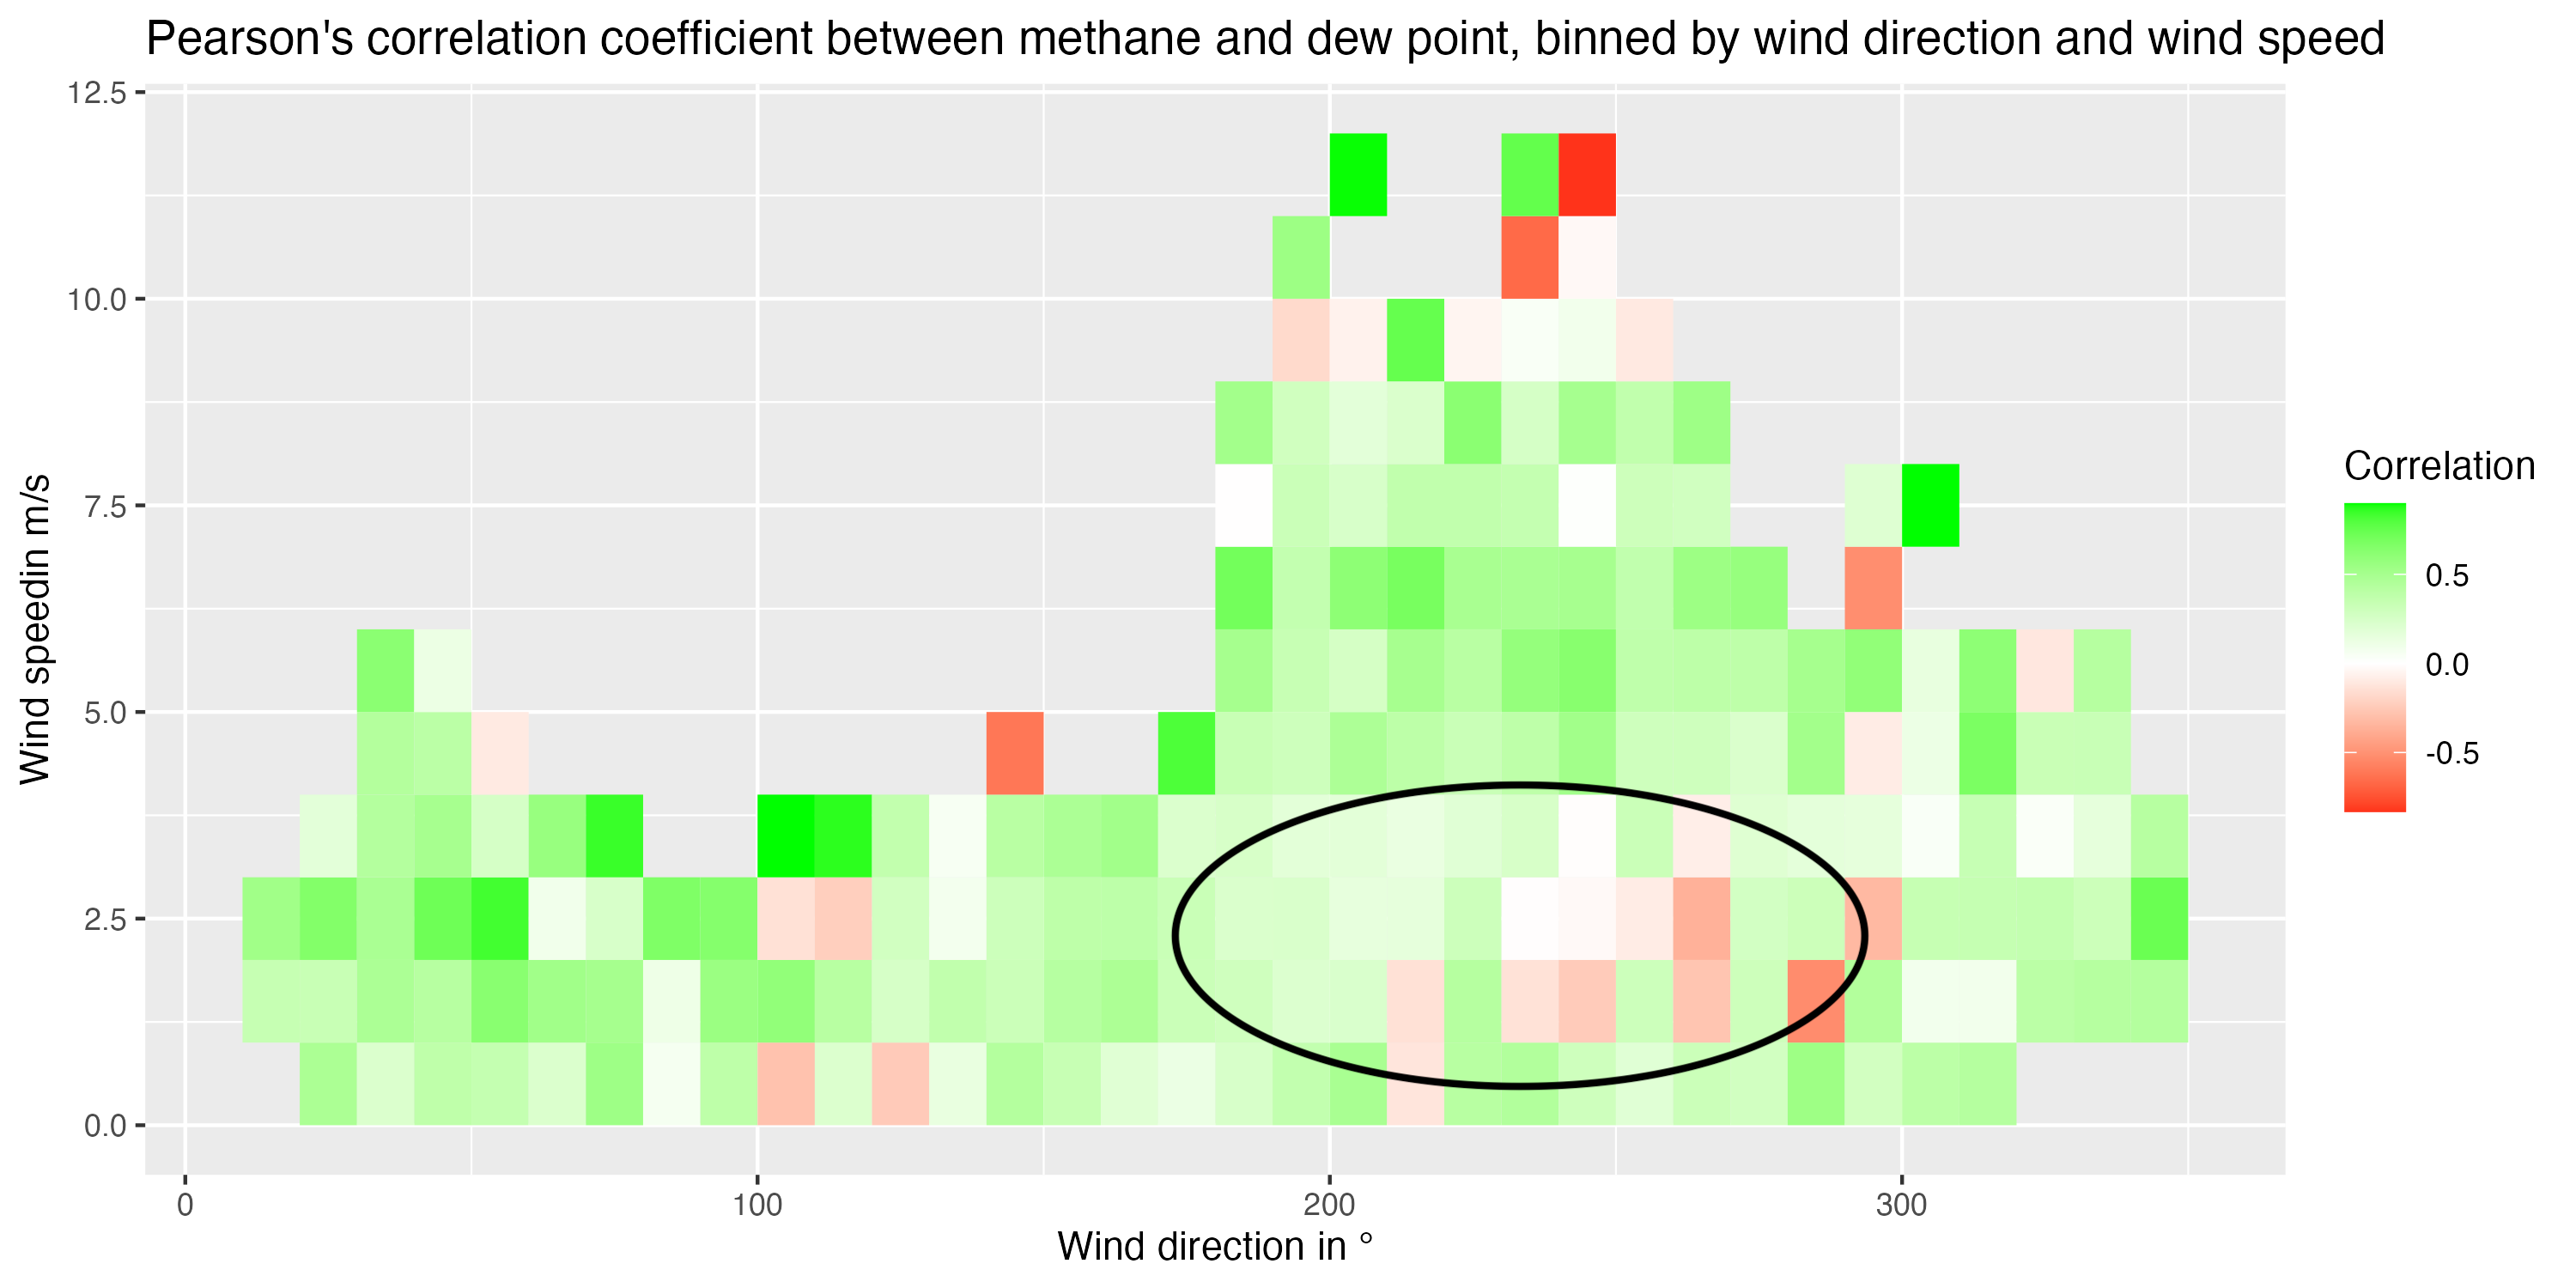
\includegraphics[width=.48\linewidth]{figures/Appendix/Meteorological/13_CH4_vs_dew_point_Correlation_Geomatikum.png}%
        \label{CorrDewPoint}%
    }\\
    \subfloat[Air temperature]{%
        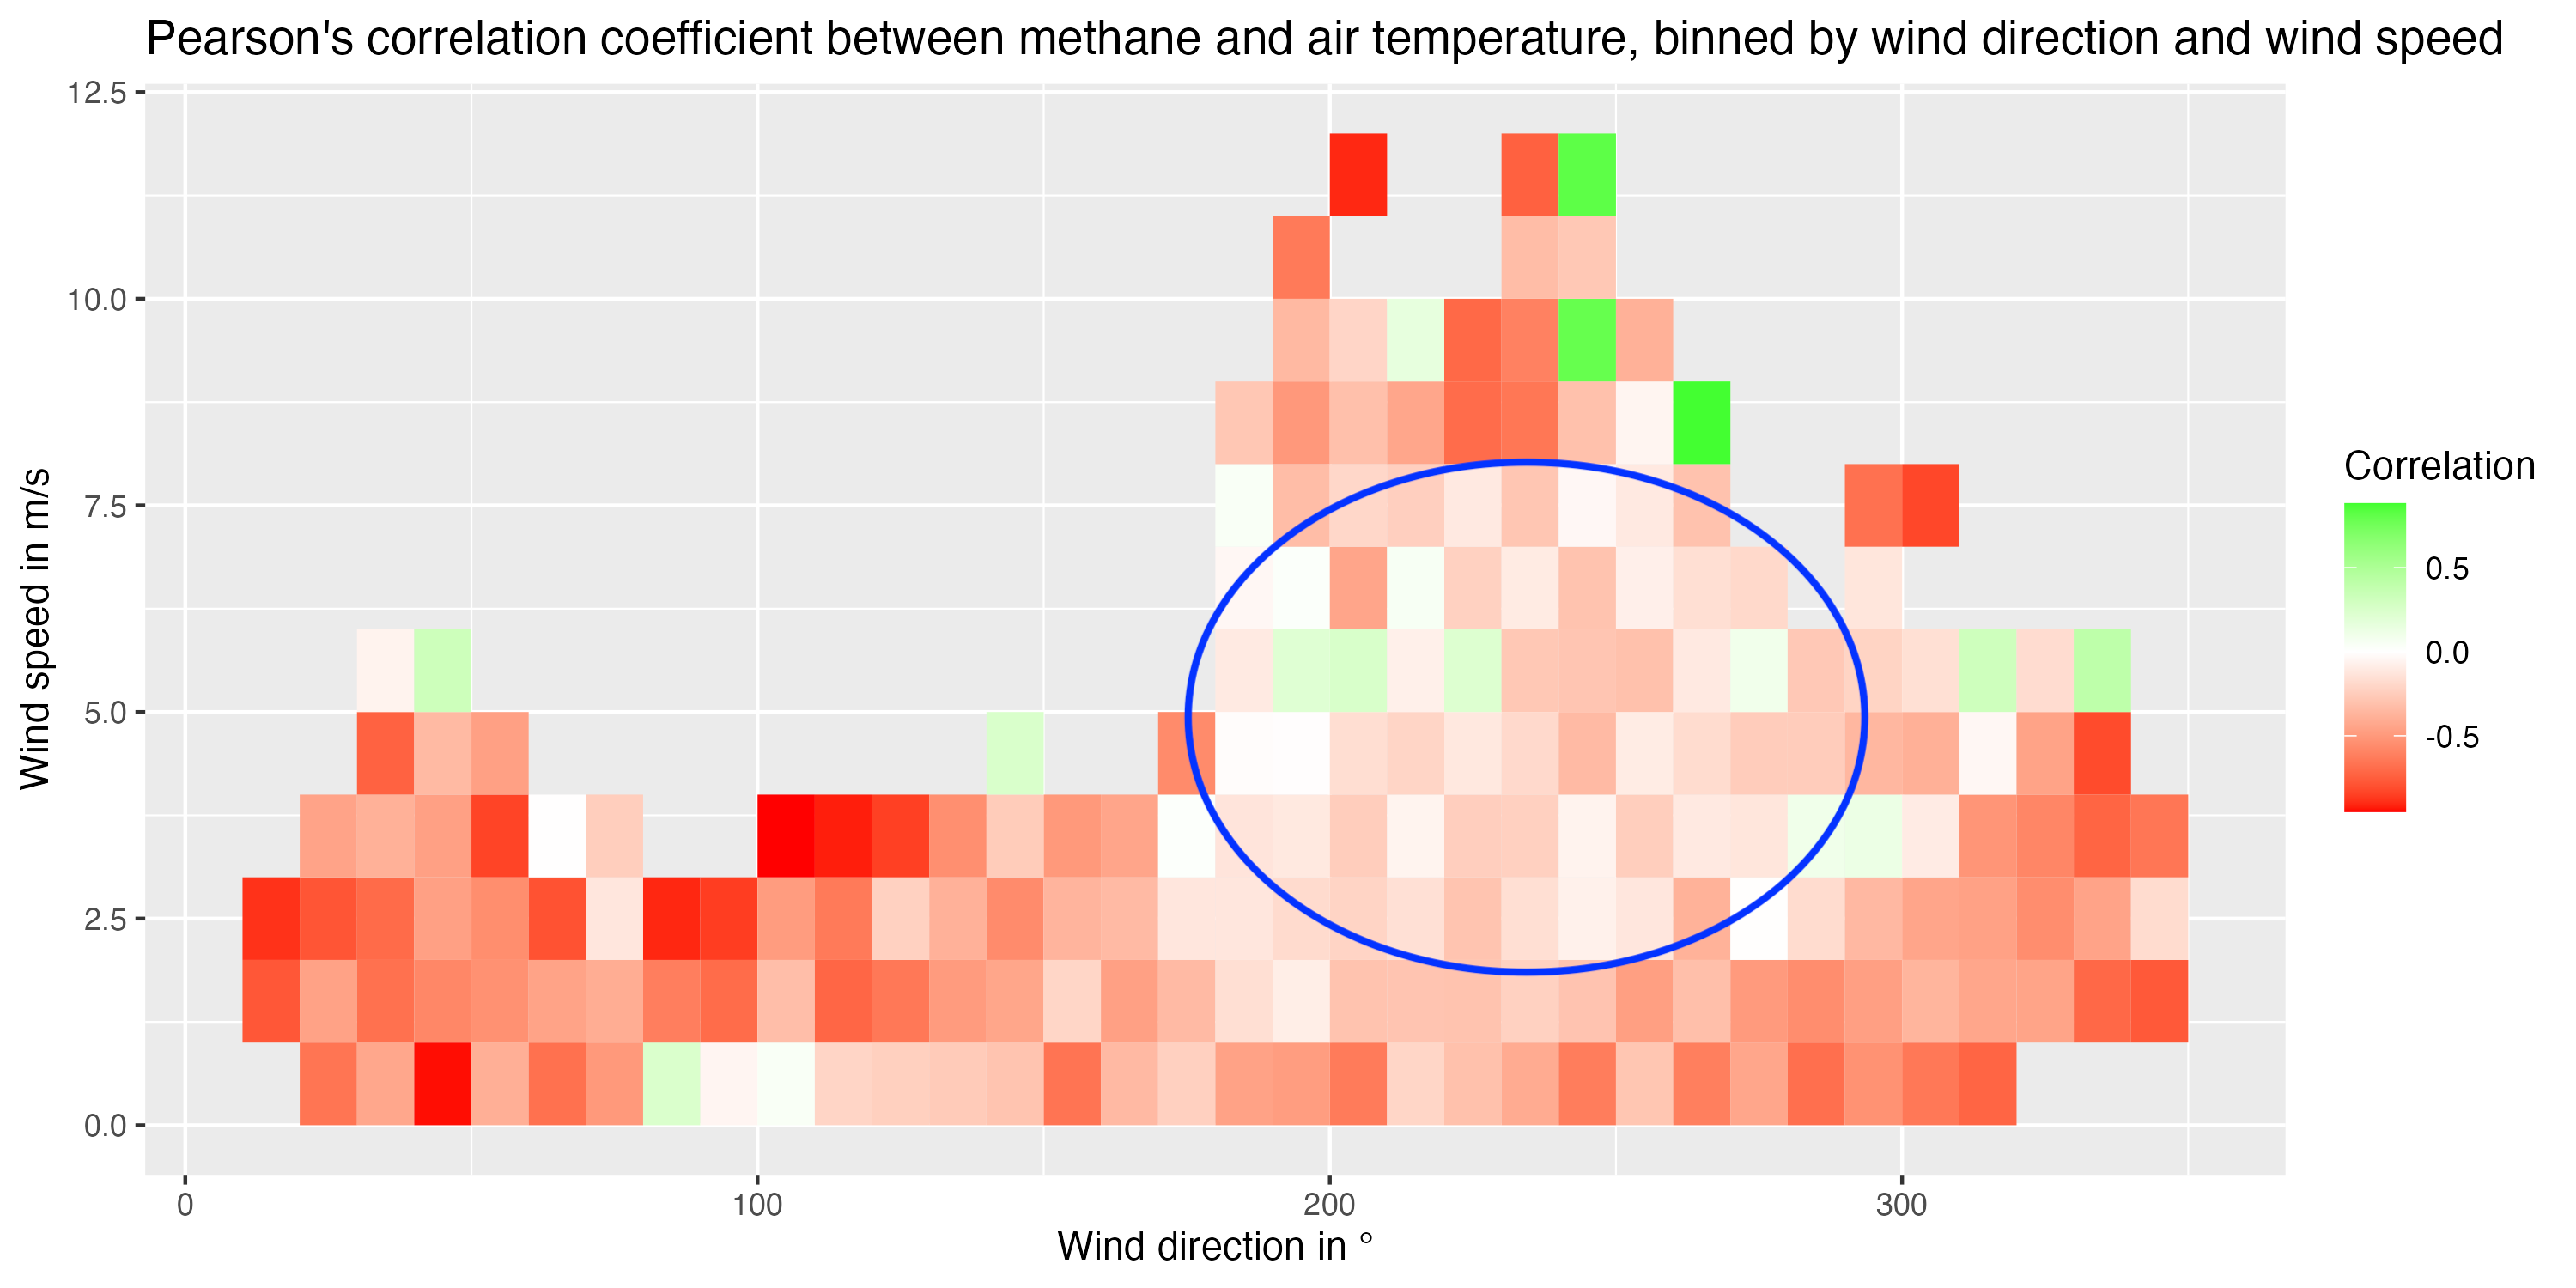
\includegraphics[width=.48\linewidth]{figures/Appendix/Meteorological/13_CH4_vs_temperature_Correlation_Geomatikum.png}%
        \label{CorrAirTemp}%
    }\hfill
    \subfloat[Radiation]{%
        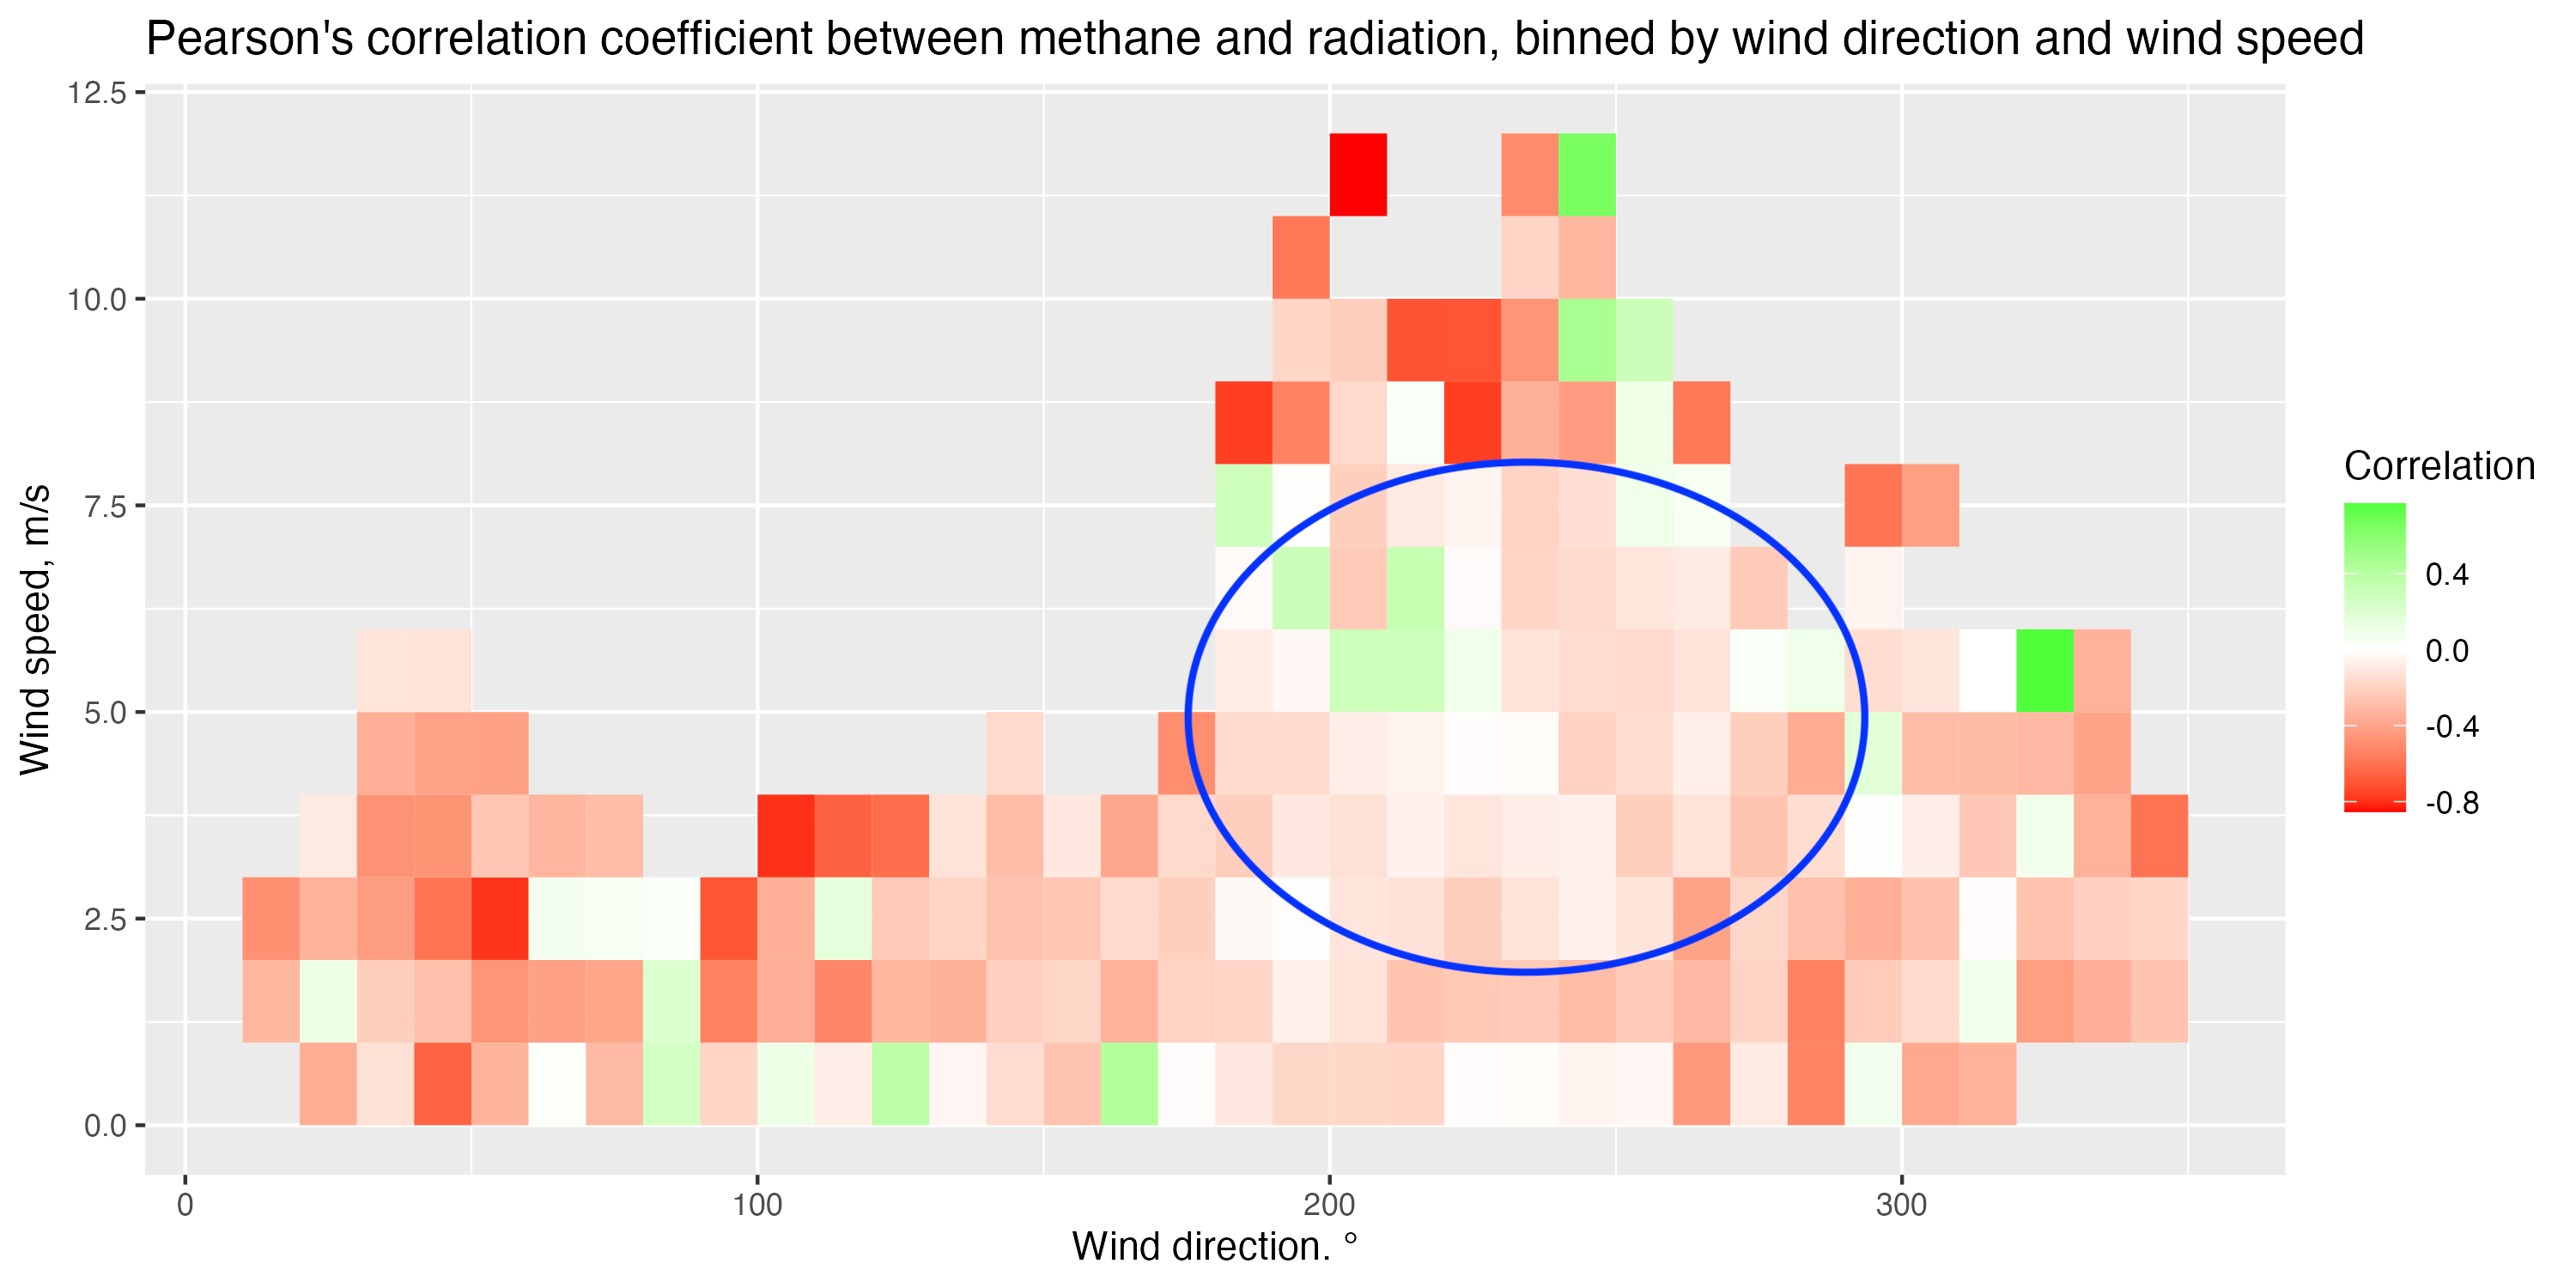
\includegraphics[width=.48\linewidth]{figures/Appendix/Meteorological/13_CH4_vs_radiation_Correlation_Geomatikum.png}%
        \label{CorrRadiation}%
    }
    \caption[Correlation between CH$_4$ and meteorological data]{Pearson's correlation coefficient between methane-air concentration and Meteorological data, binned by wind direction and wind speed. Green shows a positive correlation (enhanced CH$_4$ at high values), and Red shows a negative correlation (enhanced CH$_4$ at low values). The black circles indicate a region with no correlation, potentially the city centre of Hamburg. The blue circles indicate the region where the Elbe is located.}
    \label{CorrelationMeteorological}
\end{figure*}
Other meteorological parameters were investigated, such as precipitation and air pressure, etc. For those parameters, no correlation with the methane concentration in the air measured at the Geomatikum could be observed.

\subsection{Wind analysis and methane correlation}
By analysing and implementing the wind measurements provided form the DWD and Hamburg Universiät, the data measured at the Geomatikum proved to yield the most reliable results. The measurements by the DWD at Hamburg-Fuhlsbüttel suffered from its low measurement altitude consequent high variability due to disturbances by the topography, \cref{WindRoseAppendix}. The measurements at the weather mast in Hamburg Billbrook showed good turbulent-free results. But due to the large distance between the CF-IRMS measurement location and the weather mast of 17 km the measurements showed a temporal mismatch between the two measurement series. The measurements at the Geomatikum proved the most reliable due to proximity to the CF-IRMS measurement and the relatively low disturbance due to the measurement height of 83m. In the modelling, discussed later on, the measurements at the Geomatikum also showed the best results.\\
The total measurement series from 01.08.21 to 01.4.2022 showed that dominant wind direction could be observed from the South-West with generally medium wind speeds. The Windrose Plot \cref{RoseTotalGeomatikum} show this average wind direction from South-West rather well. While wind from all directions has generally been observed, four distinct patterns were observed, indicating some reoccurring and distinguished weather patterns in Hamburg. Most likely, the westerly winds, high-pressure regions over the mainland and transitions of cyclones into central Europe. By additionally using the methane measurements in a pollution rose plot, one can see that the methane emission does come from every direction with a distribution closely reassembling the wind direction distribution. This shows us that the background methane concentration has no clear emission direction. While the highest concentrations are generally observed more often in South-Western wind directions.
\begin{figure}
\centering
\begin{subfigure}{.5\textwidth}
  \centering
  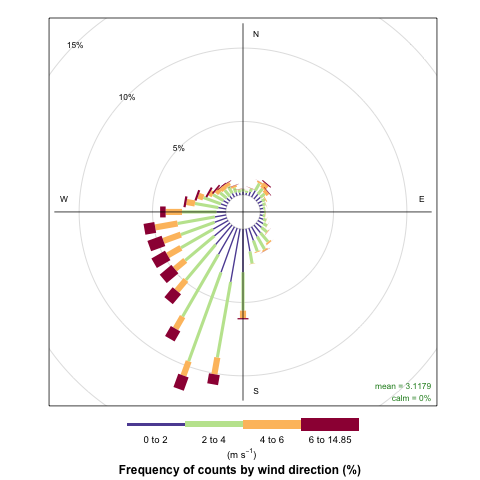
\includegraphics[width=1\linewidth]{figures/Appendix/Windrose/WindRose_Total_medium_peaks.png}
  \caption{}
  \label{WindroseTotal}
\end{subfigure}%
\begin{subfigure}{.5\textwidth}
  \centering
  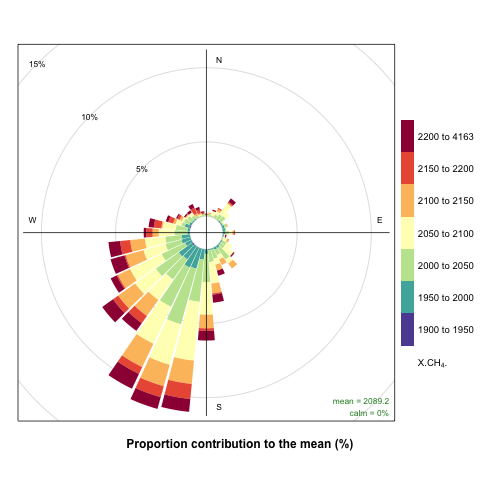
\includegraphics[width=1\linewidth]{figures/Appendix/Windrose/PollutionRose_Total_medium_peaks.png}
  \caption{}
  \label{PollutionroseTotal}
\end{subfigure}
\caption[Windrose and Pollutionrose for total timeline at Geomatikum]{(a) Windrose for the total campaign measured at the Geomatikum. (b) Pollutionrose with wind data measured and CH$_4$ concentration measured at Geomatikum in ppb. }
\label{RoseTotalGeomatikum}
\end{figure}
When  applying the Peak finding algorithm with the strict identification criteria to the wind measurement data, the windrose distribution changes substantially \cref{RosePeaksGeomatikum}. Measurements from the northern with directions are  observed very rarely. Generally, only wind measurements between the South and West are observed regularly. The wind speed is also significantly slower, where most measurements have a speed of 2-4 m/s.\\
The pollution rose plot \cref{PollutionrosePeaks}, in particular, shows that the peaks, especially the high concentration ones, occur in Three distinct directions, South-west and South-South-East. The highest methane concentration peaks above 2600 ppm occurred in wind directions of South-South-West. In this direction, the Elbe is in closest proximity to the Geomatikum. In the South-South-East to the Geomatikum, the city centre with its numerous channels, fleets and small ports is located. This waterbody in this region experiences the effect of the tide strongly.\\
The directions observed in the pollution rose plots are the same as the ones observed in the correlation plot in \cref{MethaneWaterLevel}, correlating the water level and quality with the Methane concentration in the air. This is another indication that the methane observed at the Geomatikum originates at the Elbe.
\begin{figure}
\centering
\begin{subfigure}{.5\textwidth}
  \centering
  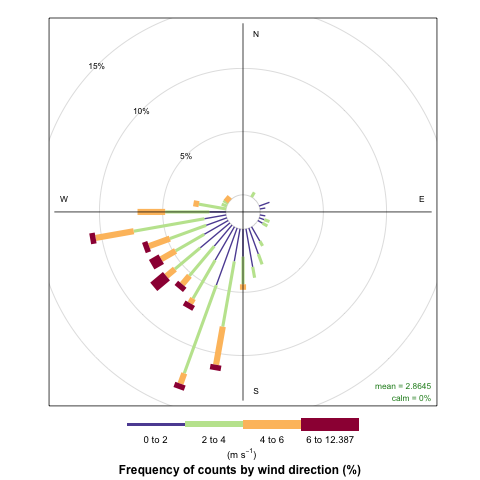
\includegraphics[width=1\linewidth]{figures/Appendix/Windrose/WindRose_Peaks_medium_peaks.png}
  \caption{}
  \label{WindrosePeaks}
\end{subfigure}%
\begin{subfigure}{.5\textwidth}
  \centering
  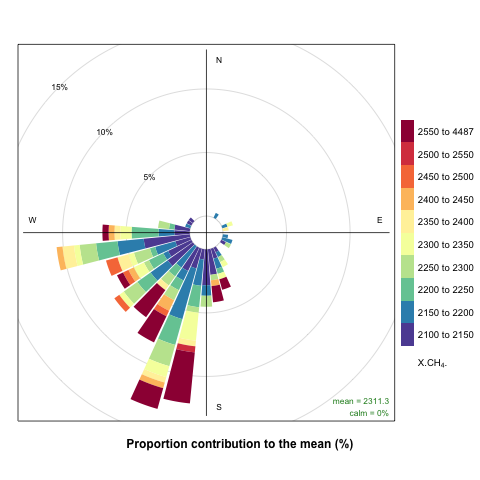
\includegraphics[width=1\linewidth]{figures/Appendix/Windrose/PollutionRose_Peaks_medium_peaks.png}
  \caption{}
  \label{PollutionrosePeaks}
\end{subfigure}
\caption[Windrose and Pollutionrose for total timeline at Geomatikum]{(a) Windrose during CH$_4$ peaks identified with strict criteria measured at the Geomatikum. (b) Pollutionrose for the CH$_4$ peaks with wind data measured and CH$_4$ concentration measured at Geomatikum}
\label{RosePeaksGeomatikum}
\end{figure}

\section{Methane Transport modeling}
\subsection{Source distance estimation}
With the use of the distance estimation model, the distance between the methane peak emission location and the Geomatikum was modelled. The resulting plot can be seen in \cref{DistancePlot}. In this plot, each point represents an individual methane peak with its methane concentration measured at the Geomatikum versus the estimated distance between the emitter and measurement location. The blue line represents a local regression with its standard errors highlighted in dark grey. For this plot, strict peak identification criteria are used. A plot with the identification criteria as described by \cite{Menoud.2021} can be seen in \cref{DistancePlotPaperAppendix}.
\begin{figure}[htbp]
 \centering
 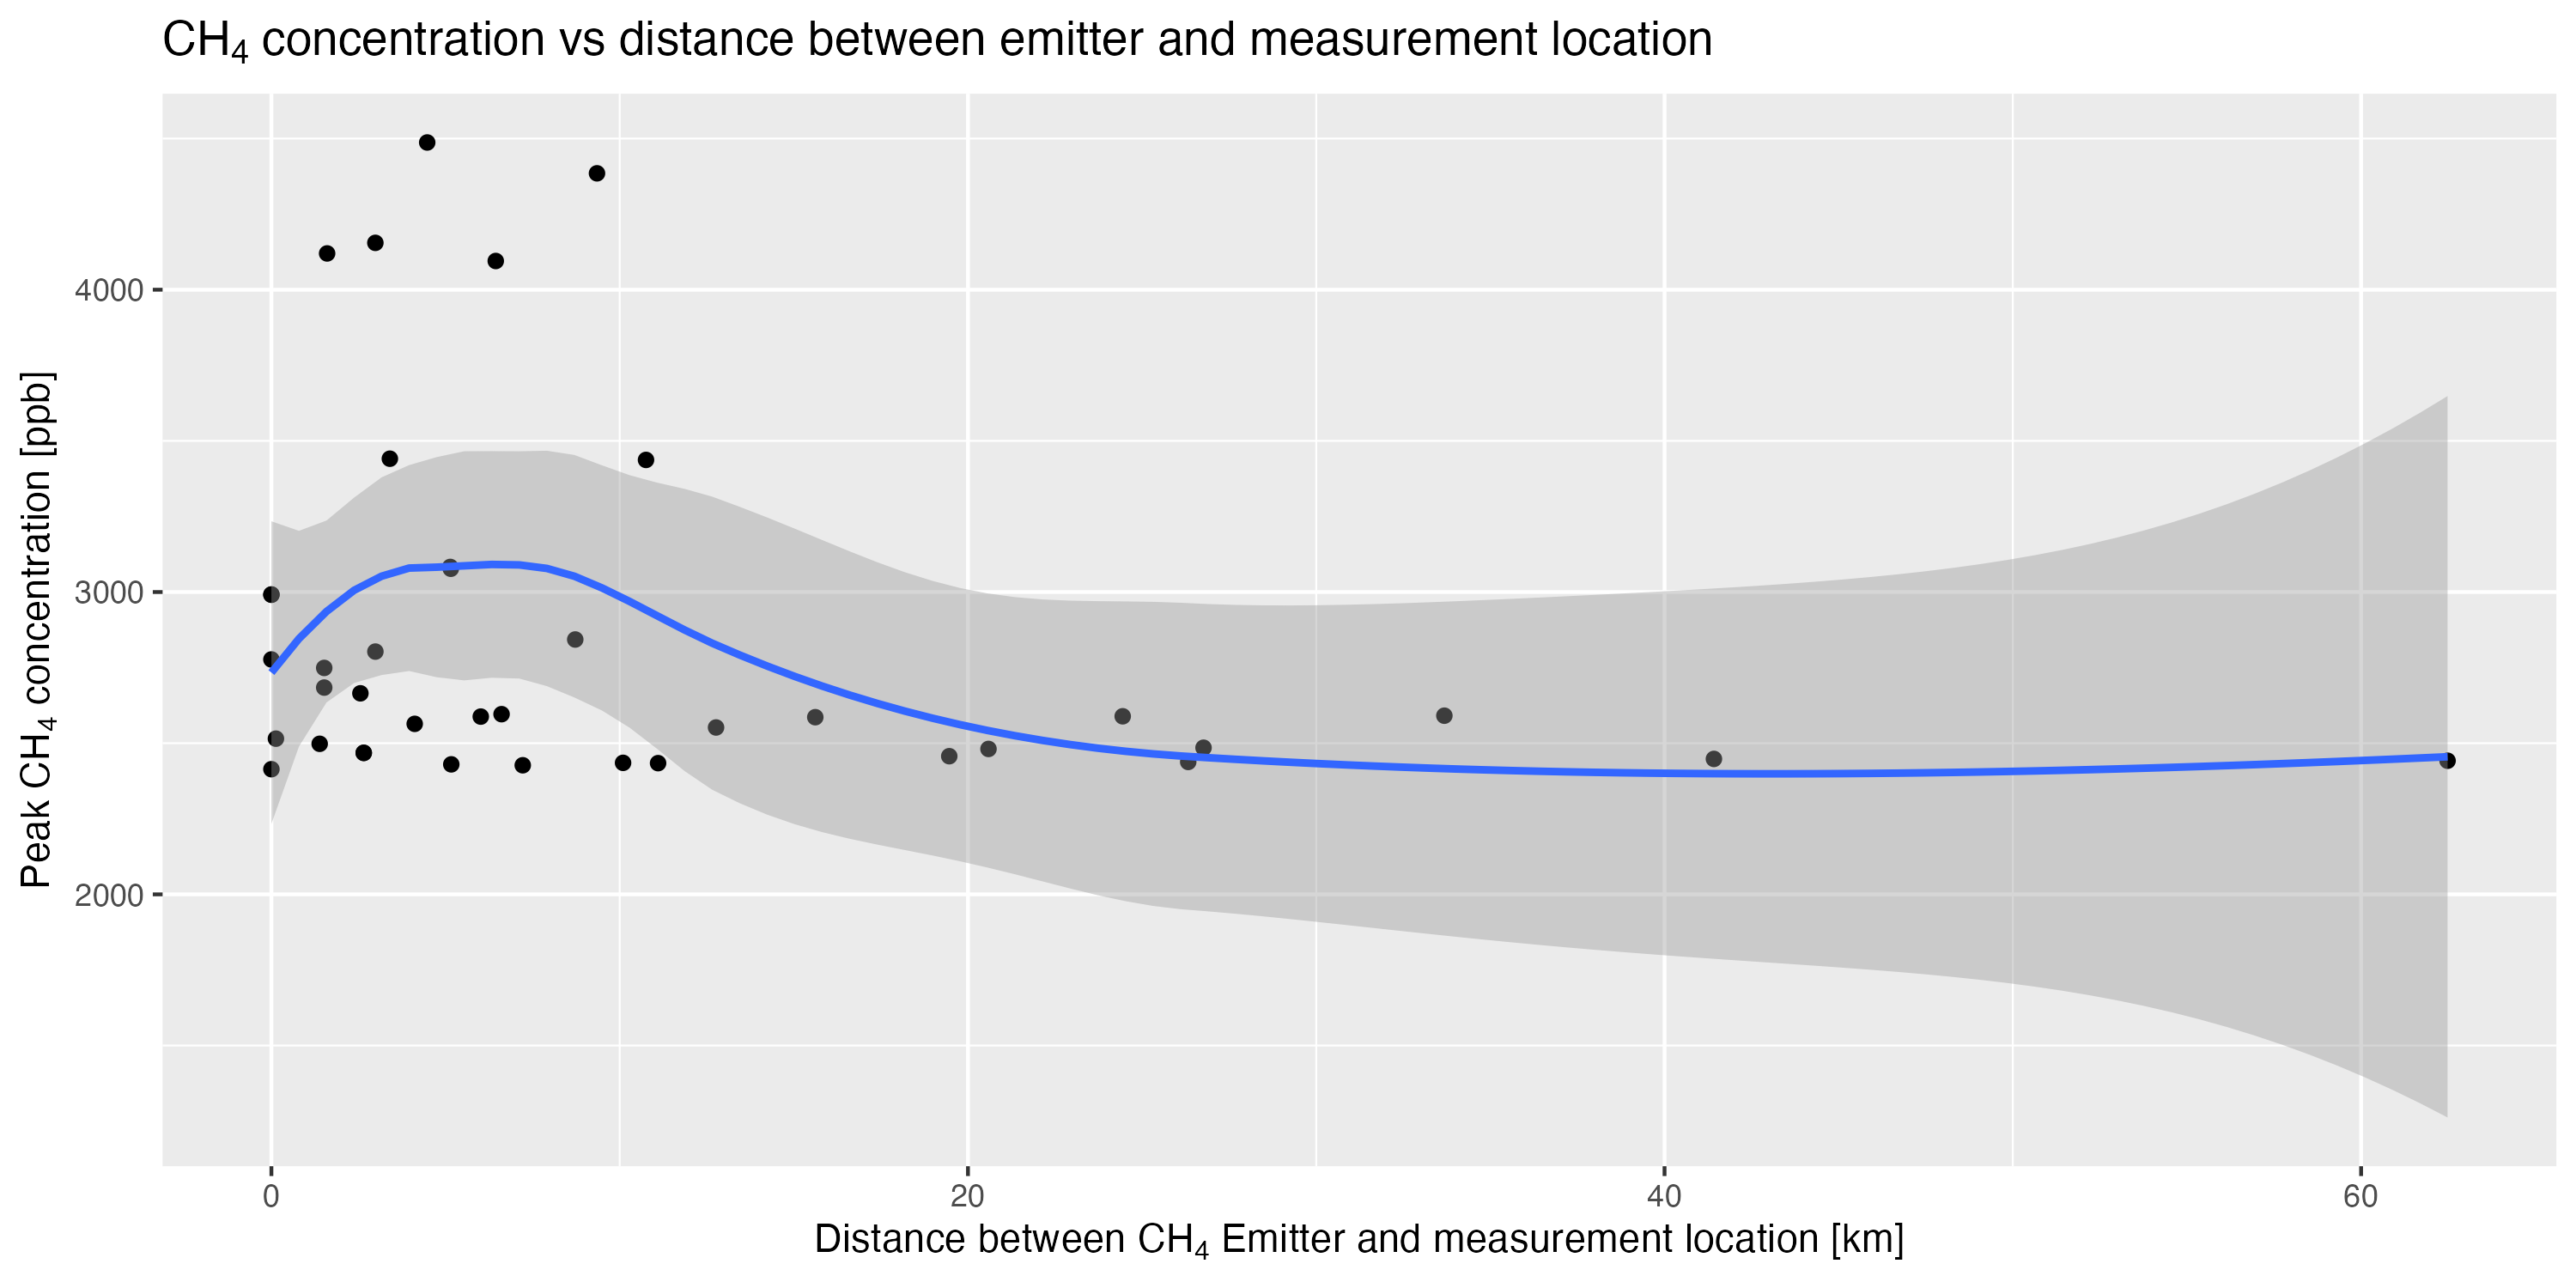
\includegraphics[width=1\textwidth]{figures/Appendix/Transportmodel/14_Low_WL_to_Peak_distance_strict_peaks.png}
 \caption[Distance between estimated emitter and measurement location]{Scatter plot of modelled distance between the estimated emission location and the measurement location at the Geomatikum, against the methane concentration observed at the Geomatikum measured by the CF-IRMS. A local regression line is fitted to the plot (blue),  showing the highest concentration peaks to be emitted at a distance of 5$\pm$3 km. The standard error of the line is shown in dark grey. The peaks were identified using the strict identification criteria.}
 \label{DistancePlot}
\end{figure}
A few details can be observed from the plot. The highest density of peaks is seen between 2 and 10 km distance with a rapidly decreasing density with an increase in distance. A couple of peaks show large distances of up to 60 km away. The distance estimation for those points is most likely not correct as the distance travelled is substantial, and the plume of a  strong and  localized methane emitter would most likely spread considerably over this distance. A geographically large emitter such as the Waddensea is in the 60 km range, and large emissions from this region could, at favourable wind conditions, result in an elevated methane concentration in the air. A possible distance overestimation due to strong winds for a close-by emitter is also possible.\\
The methane concentration measured decreases with the distance. When considering the  local regression line, a peak at a distance of 5 km can be observed. The curve also shows that the peaks estimated to originate further away have a decreasingly lower methane concentration. This curve indicated that the emission location responsible for the high concentration peaks is located at a distance of around 5$\pm$3 km from the Geomatikum. In a 5 km radius of the Geomatikum, most of the Hamburg port, the channels fleets etc., are located. While a 10 km radius includes most of the Waterbodies located in Hamburg.

\begin{comment}
   The distribution changes sustainably when applying the peak identification criteria described in the literature by \cite{Menoud.2021}. While most peaks are estimated relatively close to the measurement location, a high concentration can be measured at a distance of up to 100 km. Some outlier peaks have an estimation of 370 km. The concentration dose again decreases with distance, with the highest concentration under 20 km.
Using this plot, it has to be assumed that the peak identification criteria identified many peaks that don't seem to originate from the Elbe and have a different production mechanism.\\
The plot nether the less helps us to define a boundary for the transport modelling of maximal 60 km from the measurement location. A greater distance would be subject to too many variables.\\ 
\end{comment}

\subsection{Emitter location modeling}
 The transport of the methane has been modelled and is shown in  \cref{TransportmodelStrictPeaks}. In this plot, only the methane peaks identified with the strict identification criteria are modelled. The density distribution represents the probability of the methane emission locations and is shown as a heatmap overlay in the figure.
\begin{figure}
\centering
\begin{subfigure}{.5\textwidth}
  \centering
  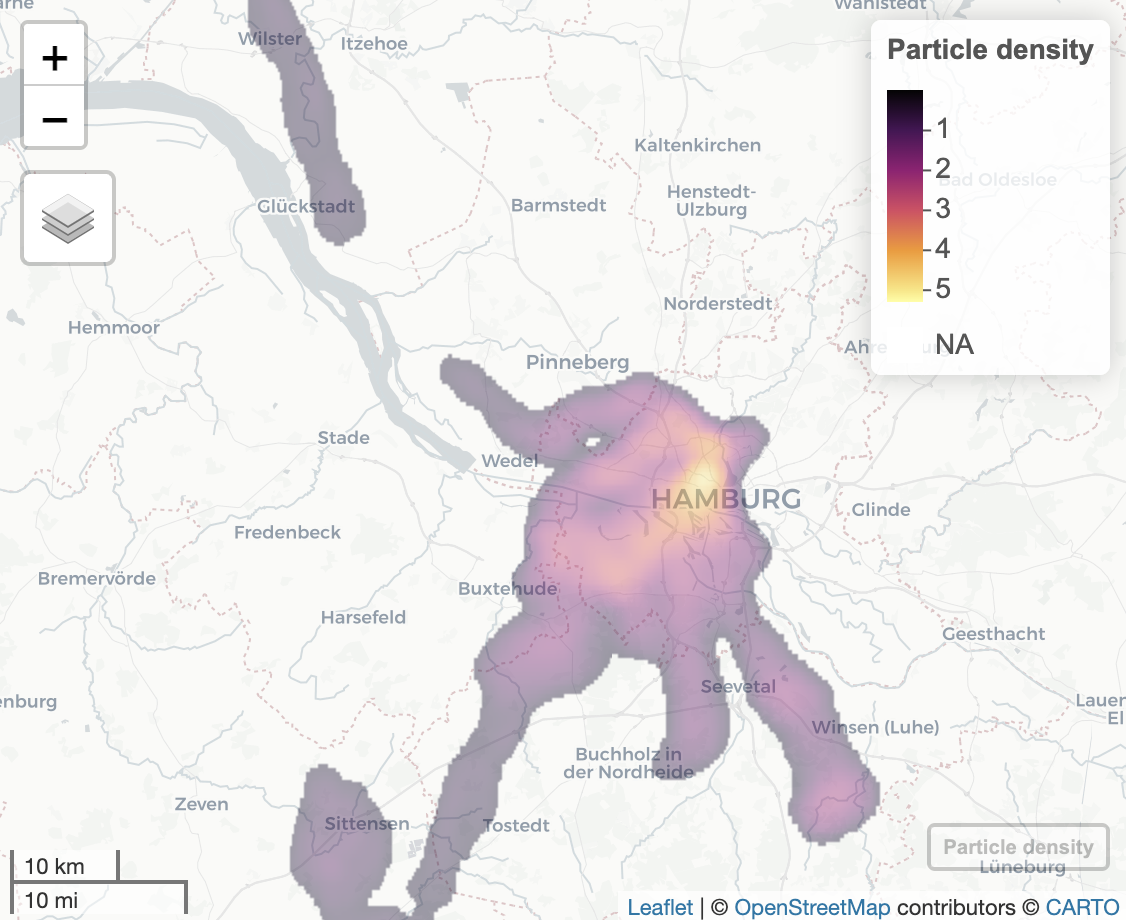
\includegraphics[width=1\linewidth]{figures/Appendix/Transportmodel/10_Emission_Distribution_with_Changing_Measured_Wind_strict_peaks.png}
  \caption{}
  \label{TransportmodelStrictPeaksLrage}
\end{subfigure}%
\begin{subfigure}{.5\textwidth}
  \centering
  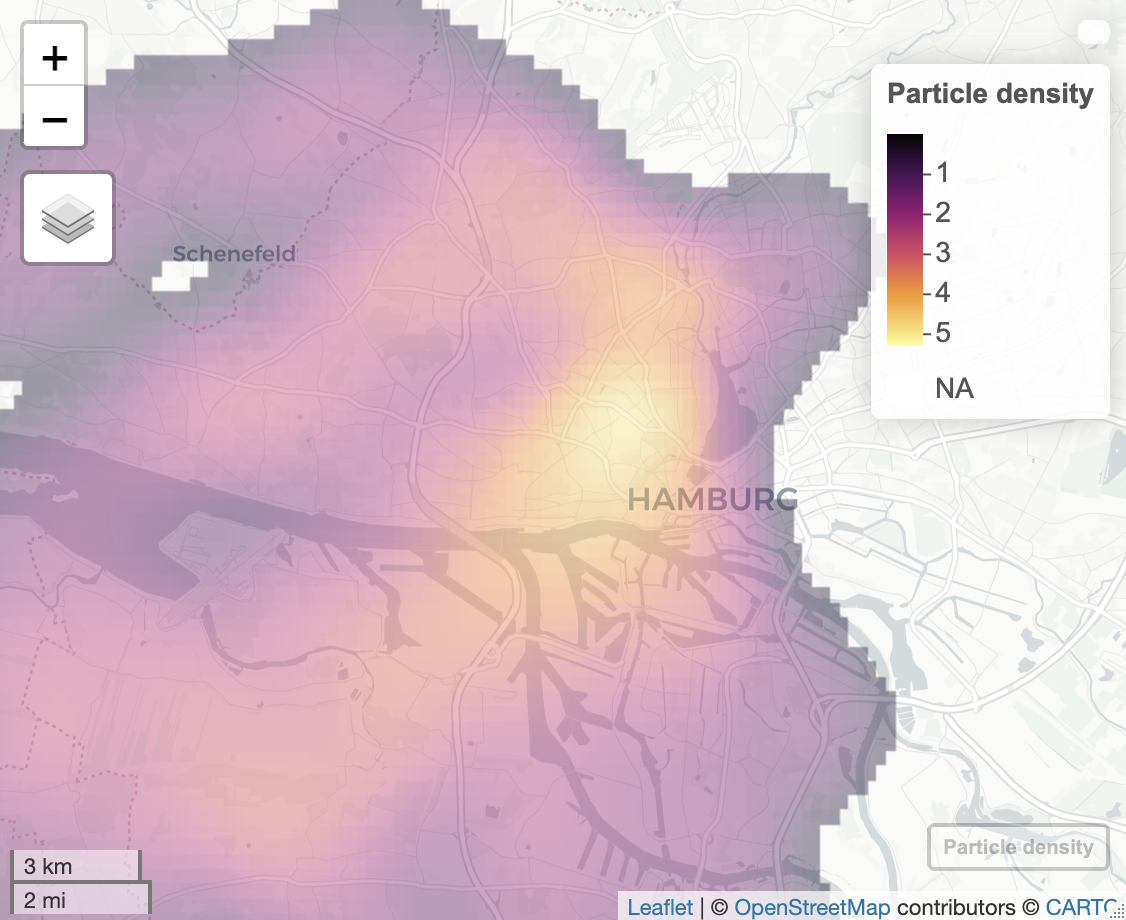
\includegraphics[width=1\linewidth]{figures/Appendix/Transportmodel/10_Emission_Distribution_with_Changing_Measured_Wind_strict_peaks_Zoom.png}
  \caption{}
  \label{TransportmodelStrictPeaksZoom}
\end{subfigure}
\caption[Transport Model]{Map of the partial density for the time-reversed Gaussian plume model. Using strict methane peak identification criteria to select only prominent methane peaks. Wind data was measured at the Geomatikum with 10 min time-averaged values. 1000 Particles released per methane peak with standard deviations of 0.5 m/s and 20°. Heat map overlay representing the particle density at each segment with a logarithmic scale. Figure (b) is zoomed into the Hamburg city region.}
\label{TransportmodelStrictPeaks}
\end{figure}
The plot shows an exceptionally high density in certain inner-city regions. 
The first is in the historic city centre, where the Alster joins the Elbe. This Part of the city has a large, sweet water lake, the Alster, which is relatively shallow. \cite{Maazallahi.2020} and the mobile measurements during the UNEP campaign consistently observed an elevated methane concentration around the Alster. While the enhancements were low in magnitude, they were spread out over a large area around the lake. The Lake and river join the Elbe by locks and controlled water management systems. This region also has many interconnected fleets, historic harbours, and channels freely connected to the river Elbe. Some of them completely dry out for some amount of time during the tide cycle, exposing a deep sediment-rich ground. \\
The second region is the south of Hamburg. The Hamburg port is located in this region, which includes a vast network of channels, contributing rivers, small harbours and some small wetlands. This region also shows an elevated density following the river Elbe upstream land inward. Locks in this region partly control the river and its tidal cycle. Still, most of it is free-flowing and experiences significant water level changes and even running dry in certain areas.\\
The last region of higher density is on the western side. Notably, many tracks follow the Elbe downstream along the Elbe towards the Waddensea. This region experiences the effects of the tide very strongly, with large regions that run dry during low tide. Most notably, some relative wetland regions outside of the city border.\\
This indicates that the origin of the methane peak can be quite far away. Still, the accumulation of methane along the river's entire length in the air is possible. It can produce a high methane concentration in the city with favourable wind conditions. One can also notice that a higher density occurs north of the Geomatikum. But further investigation of the tracks shows that the wind at those peaks is relatively slow and shows a turning wind direction. The tracks also lead to a large wetland region on the Elbe just outside the city bordered on the south-west side of the city.\\
When applying the Peak identification criteria by \cite{Menoud.2021}, identification of a distinct emission region is much more difficult. This is due to the wide range of peak types that are detected with this method. As will be discus in \cref{Keeling}, significantly more Anthropogenic emitters contribute to the smaller peaks. \cref{TransportmodelPaperPeaks} shows that the origin of those peaks, including ones from anthropogenic emitters, is less localised. The region around the Geomatikum shows a high density, with a generally high density in the Hamburg port region to the South and South-West of the Geomatikum. Coincidently this is also the dominant wind direction, as can be seen in \cref{RoseTotalGeomatikum}. The area covered by the tracks and the distance travelled by the particle is generally larger and more uniformly spread in every direction. This probably originates from the more random nature of the peaks occurring at unpredictable times and wind conditions.  
\begin{figure}
\centering
\begin{subfigure}{.5\textwidth}
  \centering
  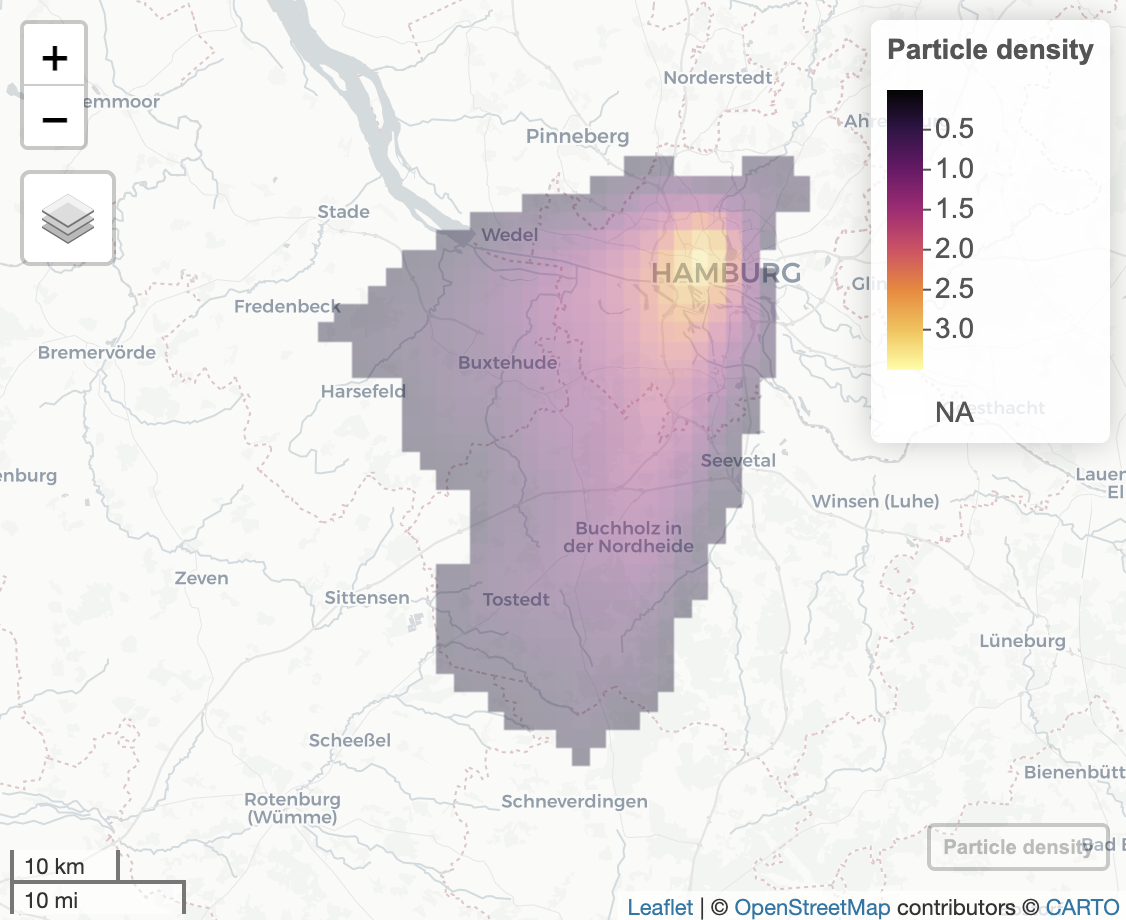
\includegraphics[width=1\linewidth]{figures/Appendix/Transportmodel/10_Emission_Distribution_with_Changing_Measured_Wind_paper_peaks.png}
  \caption{}
  \label{TransportmodelPaperPeaksLrage}
\end{subfigure}%
\begin{subfigure}{.5\textwidth}
  \centering
  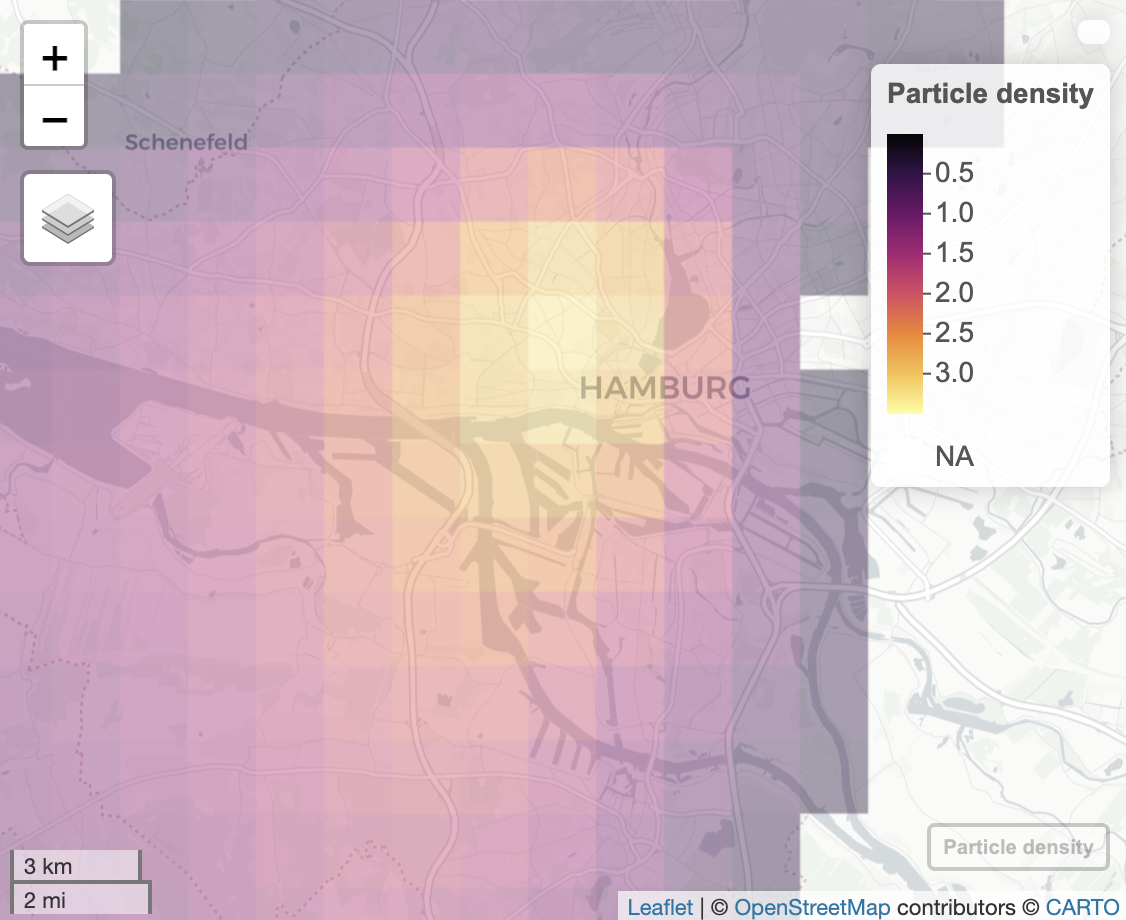
\includegraphics[width=1\linewidth]{figures/Appendix/Transportmodel/10_Emission_Distribution_with_Changing_Measured_Wind_paper_peaks_Zoom.png}
  \caption{}
  \label{TransportmodelPaperPeaksZoom}
\end{subfigure}
\caption[Transport Model with literature Peak identification criteria]{Map of the partial density for the time-reversed Gaussian plume model. Using methane peak identification criteria by \cite{Menoud.2021}. Wind data was measured at the Geomatikum with 10 min time-averaged values. 100 Particles released per methane peak with standard deviations of 0.5 m/s and 20°. Heat map overlay representing the particle density at each segment  with a logarithmic scale.}
\label{TransportmodelPaperPeaks}
\end{figure}

\section{Isotope signature analysis} \label{Keeling}
\subsection{The Keeling plot anlysis}
Using the Keeling method, the methane origin sources were investigated. The complete timeline of the $\delta$13C and $\delta$D CF-IRMS measurements together with the CH$_4$ concentration is shown in \cref{TotalIRMSTimeline}. 
\begin{figure}[htbp]
 \centering
 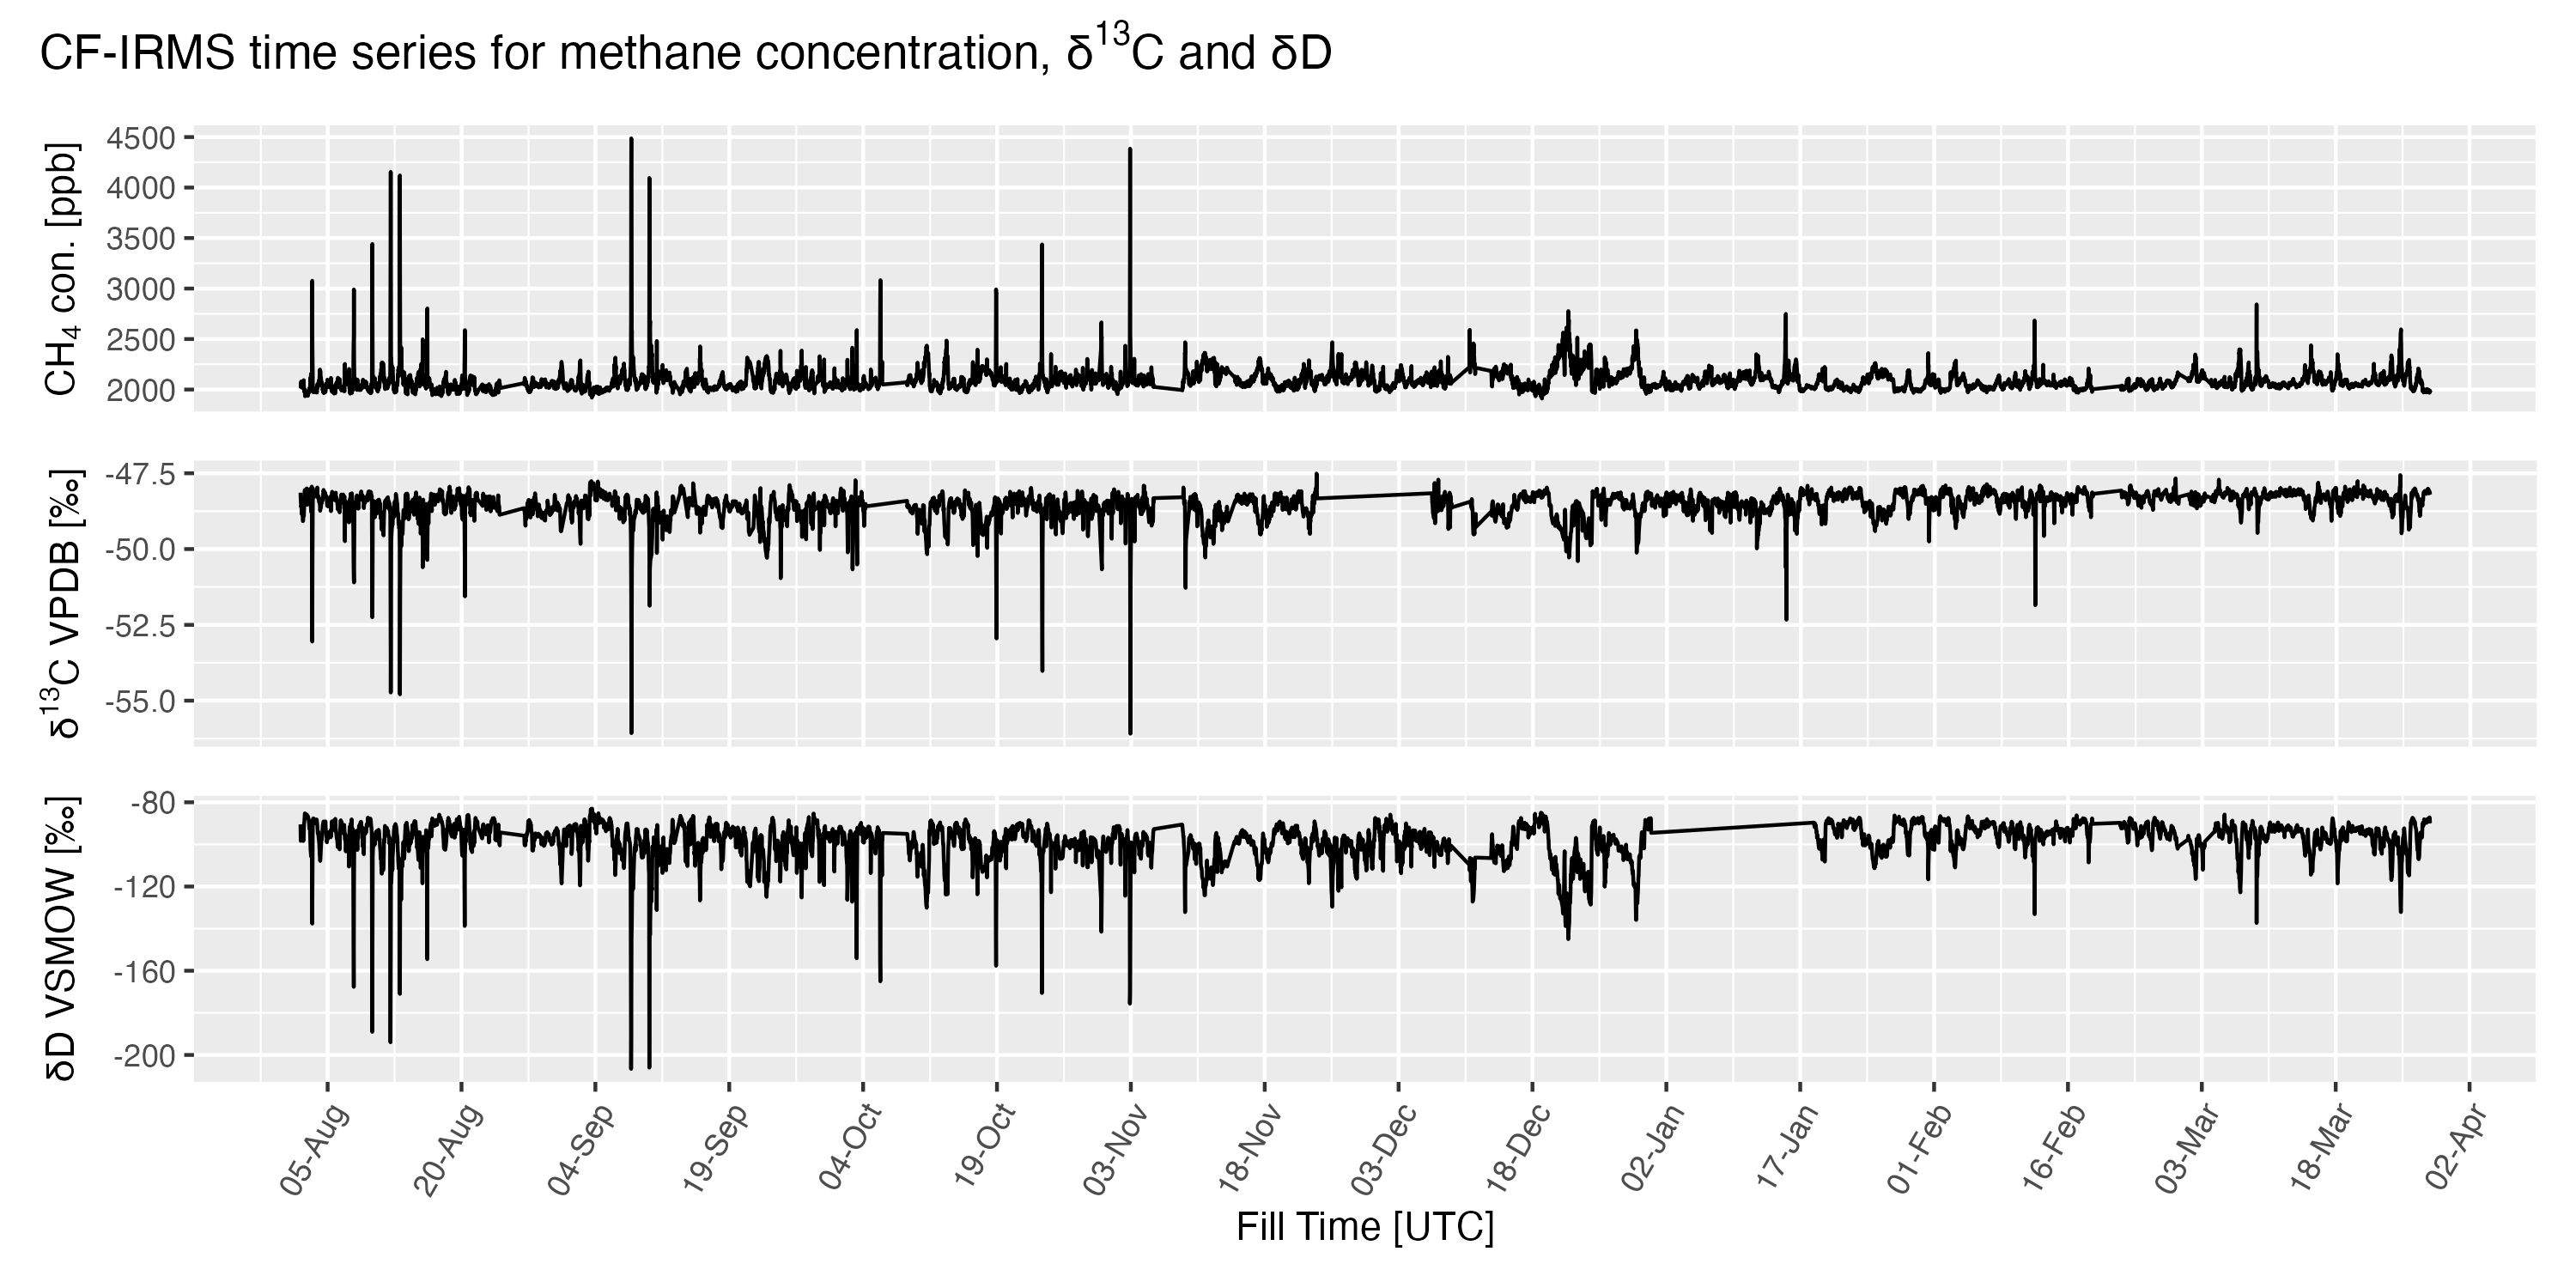
\includegraphics[width=1\textwidth]{figures/Appendix/CH4_Timelines/4_CH4_Total_Timeline.png}
 \caption[$\delta$13C, $\delta$2H and CH$_4$ timeline for CF-IRMS Measument]{Complete timeline of the $\delta$13C, $\delta$D and CH$_4$ concentration measured by CF-IRMS at Geomatikum from 1.08.2021 to 1.04.2022}
 \label{TotalIRMSTimeline}
\end{figure}
By using this complete timeline, the Keeling plot approach was deployed, and the resulting plots are shown in \cref{TolalKeelingPlot}. The isotopic signature for Carbon-13 was calculated to be $\delta$13C = -57.7$\pm $0.1$\permil$ and for Deuterium to be $\delta$D = -290.5$\pm $0.8$\permil$.  Comparing those results to the database values show that the dominant methane production mechanisms during the total campaign time in Hamburg were thermogenic and microbial CO$_2$ reduction. In particular, wetland, agriculture, and waste. Fossil fuel and other anthropogenic sources play a minor role in the composition of the methane mixture. This is surprising as Hamburg has a significant amount of heavy industry, including fossil fuel refinery, chemical industry, shipping, energy production etc.
\begin{figure}[htbp]
 \centering
 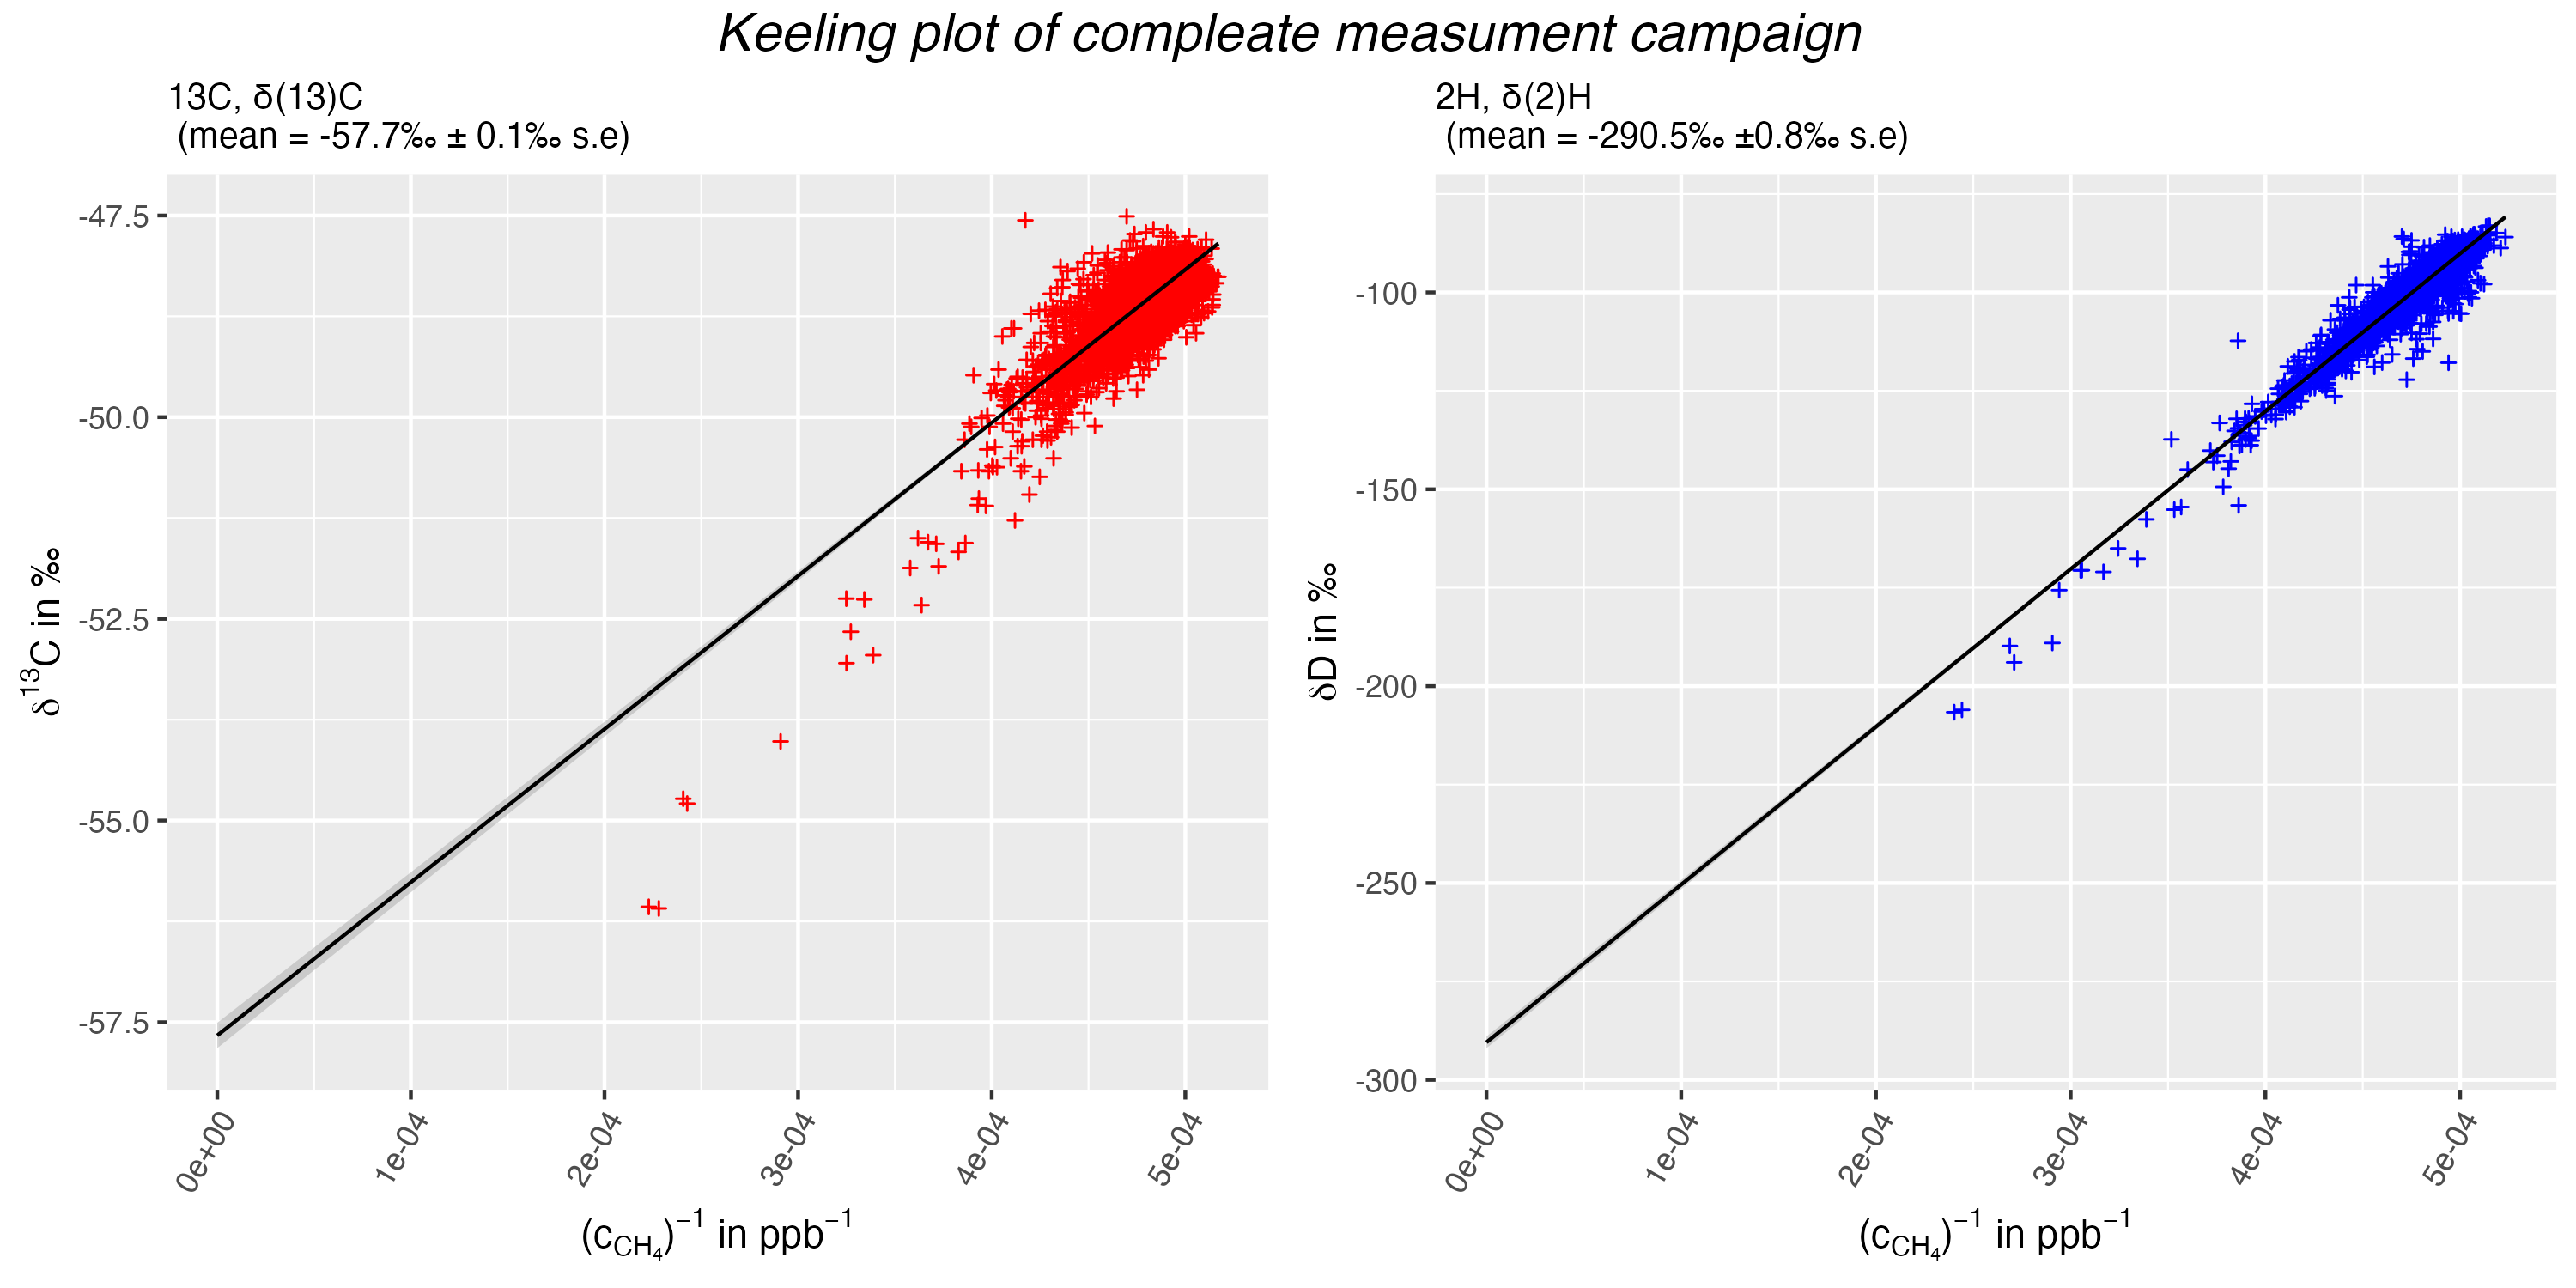
\includegraphics[width=1\textwidth]{figures/Appendix/Keeling/11_Keeling_Plot_Total_medium_peaks.png}
 \caption[Keeling Plot for total CR-IRMS measument]{Keeling Plots of Carbon-13 and Deuterium in methane measured at the Geomatikum from 1.08.2021 to 1.04.2022. The resulting isotopic signatures $\delta$13C = -57.7$\pm $0.1$\permil$ and $\delta$D = -290.5$\pm $0.8$\permil$}
 \label{TolalKeelingPlot}
\end{figure}
On the other hand, this is expected, as the surrounding countryside has significant ecocultural use, including cattle farms and large wetland and marshland areas nearby. This also includes the vast Waddensea of the German bight near the city. This Waddensea region lay upwind in the dominant wind direction to the west.\\
By applying the peak finding algorithms to the methane measurements data exclusively, the methane peaks were investigated. Here it is focused on the strict identification criteria. The Keeling plots for the identified peaks are shown in \cref{PeaksKeelingPlot}. The Keeling method shows isotopic signature for  Carbon-13  to be $\delta$13C = -60.3$\pm $0.2$\permil$ and for Deuterium to be $\delta$D = -298$\pm $2$\permil$. This indicates methane production mechanisms are much more evident in the microbial CO$_2$ reduction region and less in the thermogenic, shifting this more clearly into the wetland region, while less likely to originate from waste and agriculture. The Keeling method points toward the origin of the methane peaks due to biogenic mechanisms in the river Elbe, its contributors and the wetlands at its riverbanks.
\begin{figure}[htbp]
 \centering
 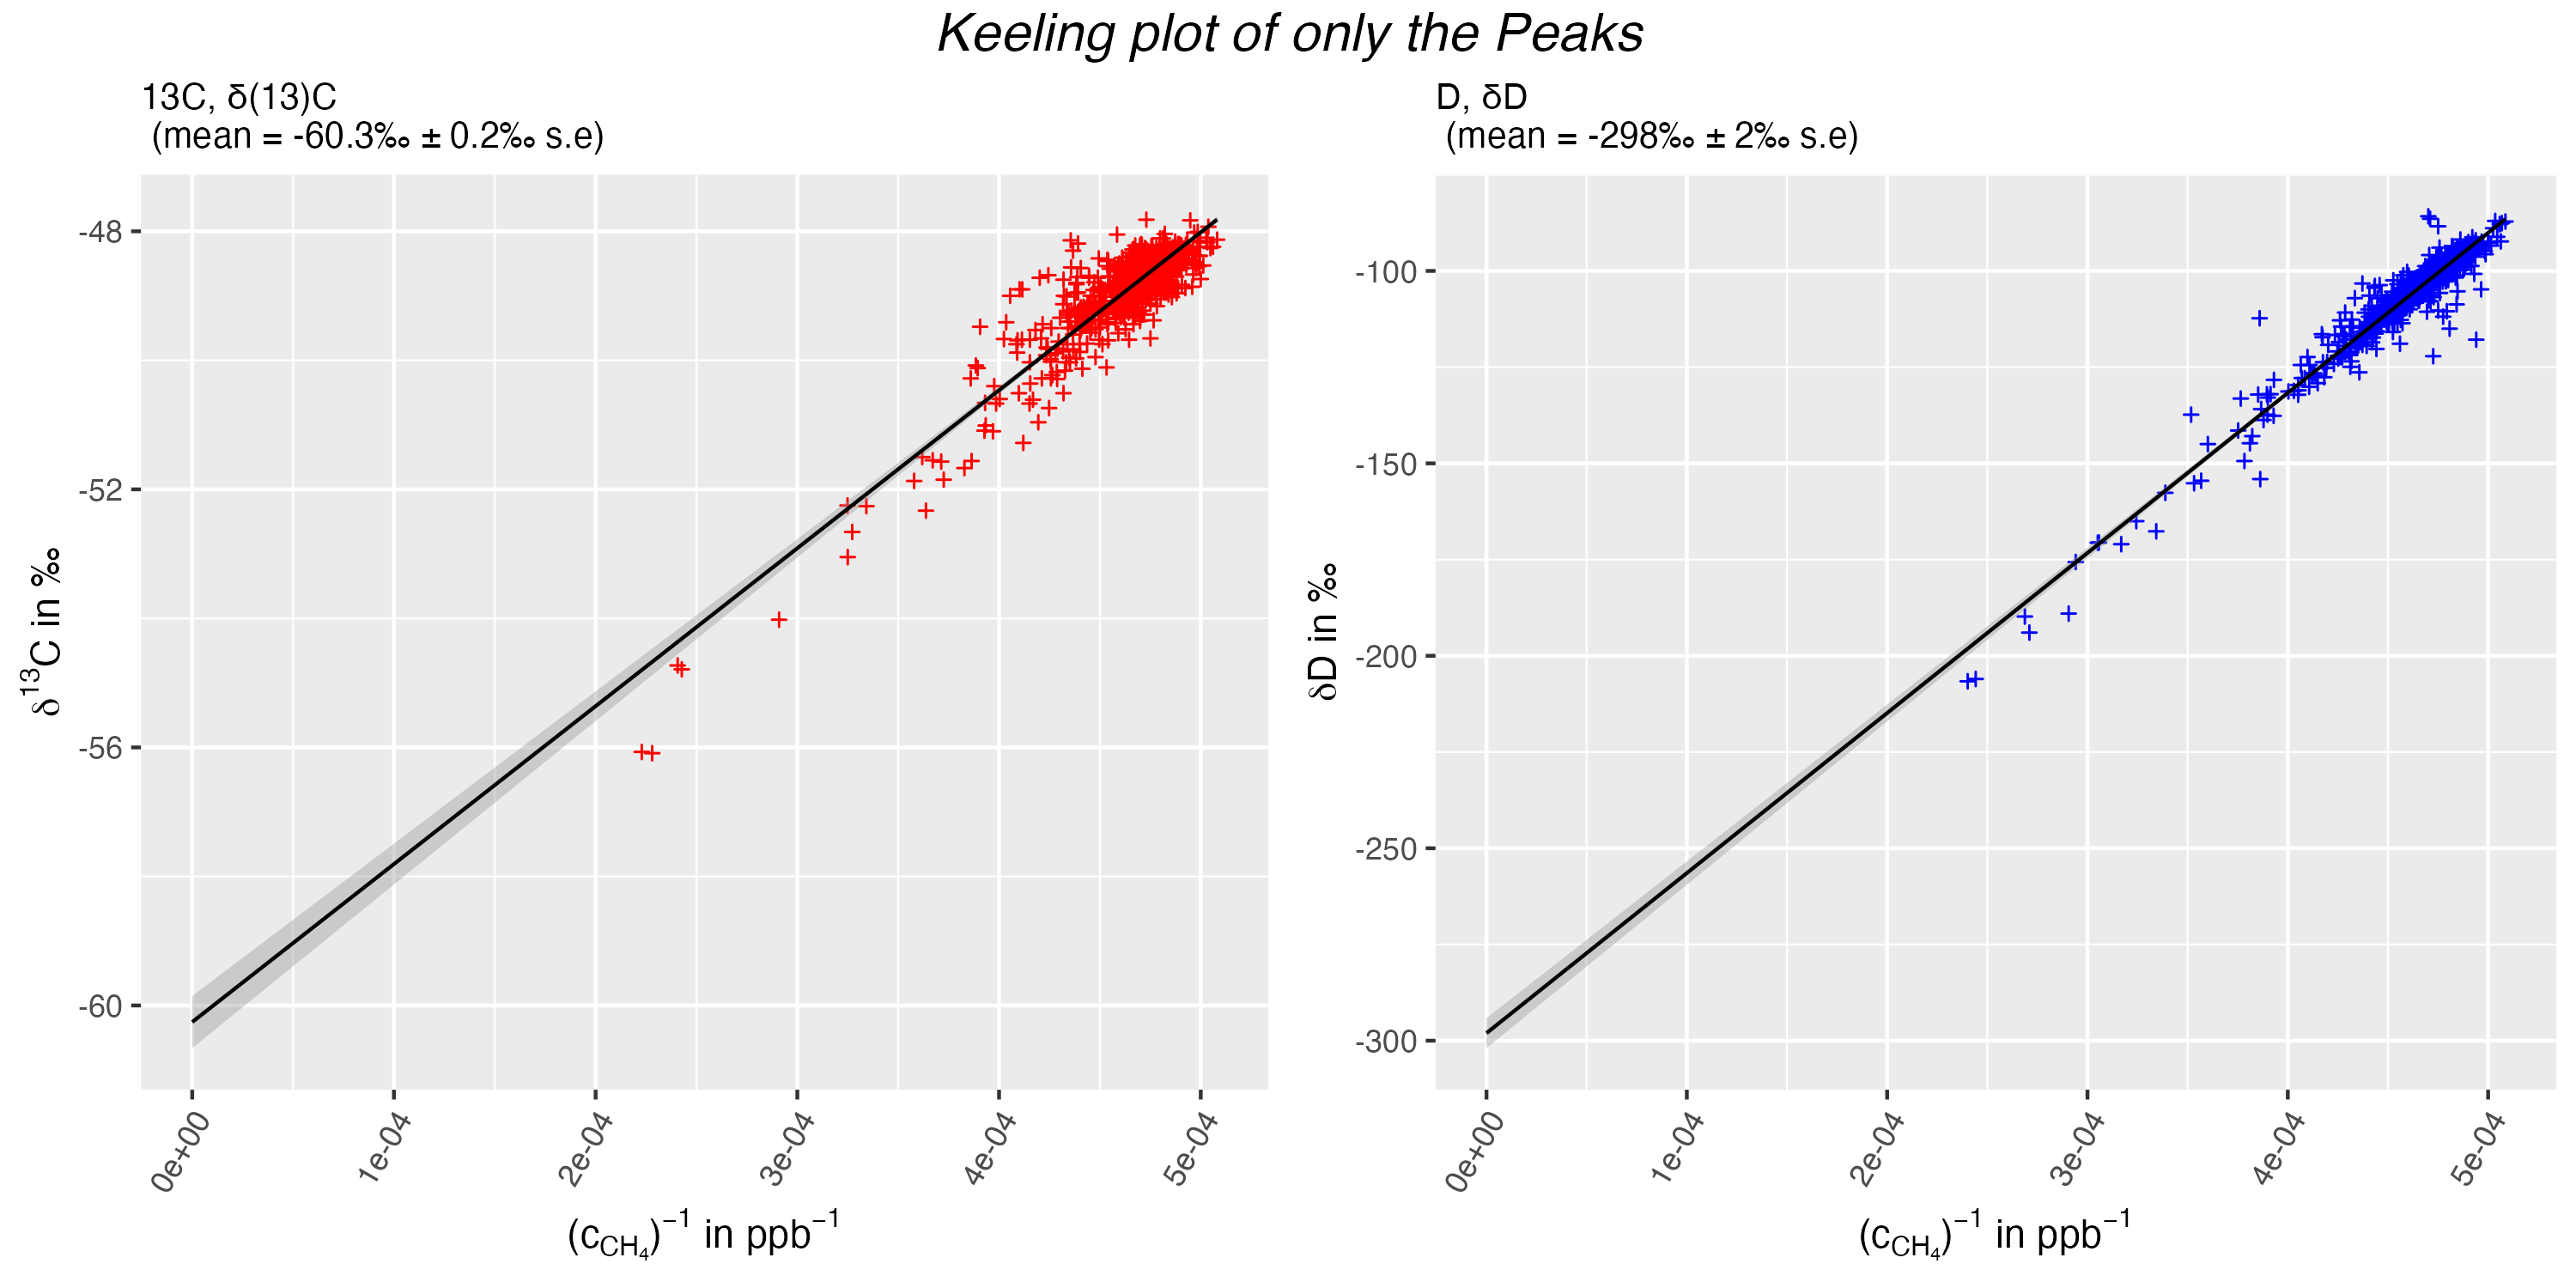
\includegraphics[width=1\textwidth]{figures/Appendix/Keeling/11_Keeling_Plot_Peaks_medium_peaks.png}
 \caption[Keeling Plot for CH$_4$ peaks in CR-IRMS measument]{Keeling Plots of Carbon-13 and Deuterium in methane peaks measured at the Geomatikum from 1.08.2021 to 1.04.2022. Strict peak identification criteria were used that only selected the prominent methane peaks. The resulting isotopic signatures $\delta$13C = -60.3$\pm $0.2$\permil$ and $\delta$D = -298$\pm $2$\permil$}
 \label{PeaksKeelingPlot}
\end{figure}
Using the wind direction makes it possible to take an even closer look at the methane emission type depending on its estimated origin location. This is done in the dual isotope plot seen in \cref{DualIsotiotopePlots}. Here a Keeling analysis for every wind direction is done within 10° bins. Each point has an error bar corresponding to its standard deviation. The point colour indicates the wind direction in regard to the North (Blue) and South (Red) wind directions. The wind directions, West and East are not considered in this plot for simplification. The Highlighted coloured areas indicate the fundamental methane production method (Microbial CO$_2$ reduction (Yellow); Microbial fermentation (Pink); Thermogenic (Dark Green) and Abiotic (light blue)). The coloured boxes show particular emitter types (Fossil fuels and non-industrial combustion (Red); Agriculture (Green); Waste (Purple); Other anthropogenic sources (dark blue); Natural wetlands (Black)). The reference database used in this dual isotope plot for the highlighted segments is from \cite{Menoud.2021}.\\
In the dual isotope plot considering the total measurement time series \cref{DualIsotiotopeTotal}, one can identify a difference in isotope signature and origin type by the wind direction. For the entire measurement series, one can see that the signature shifts to the abiotic production type for general northern wind directions, hence towards fossil fuels and other anthropogenic sources. As considerably fewer wetlands are present in this region, and many residential areas lay there, one can assume that this shifts the methane mixture towards fossil fuels. Most likely due to unburned methane from heating and cooking, leakage in the gas grid and energy generation plays a significant role in the composition of the methane mixture \cite{Lebel.2022}, \cite{Dietrich.2023}. Confirming the observations made by \cite{Maazallahi.2020} who focused on ground-based mobile measurements in the northern region of Hamburg identifying numerous methane leaks ordination from the leaks in the gas grid.
\begin{figure}
\centering
\begin{subfigure}[b]{1\textwidth}
   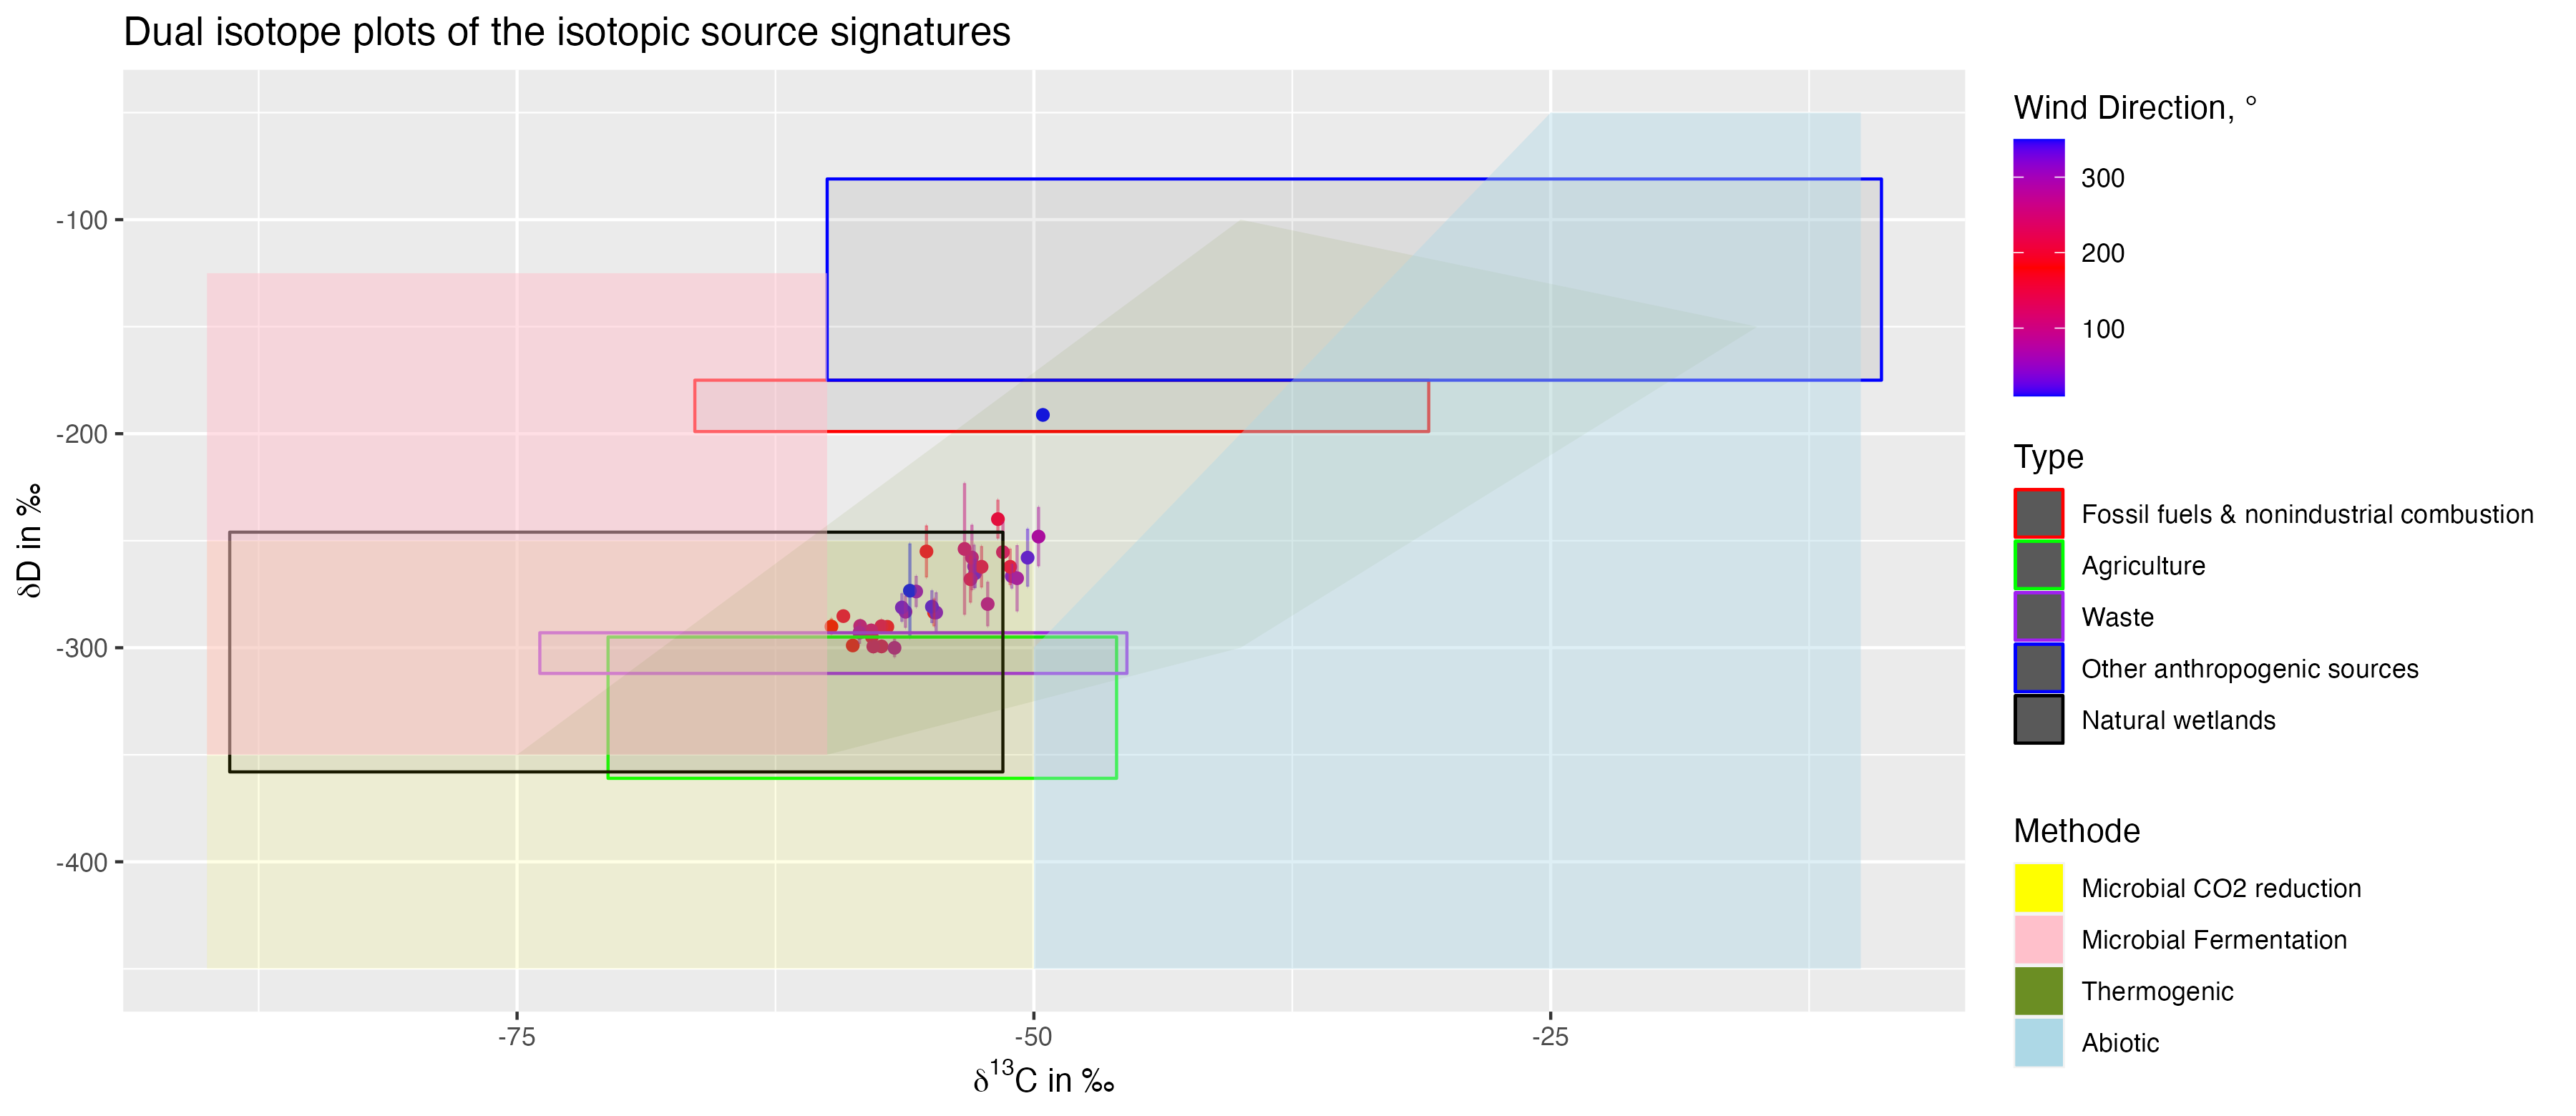
\includegraphics[width=1\linewidth]{figures/Appendix/Keeling/12_Keeling_Total_Wind_medium_peaks.png}
   \caption{}
   \label{DualIsotiotopeTotal} 
\end{subfigure}

\begin{subfigure}[b]{1\textwidth}
   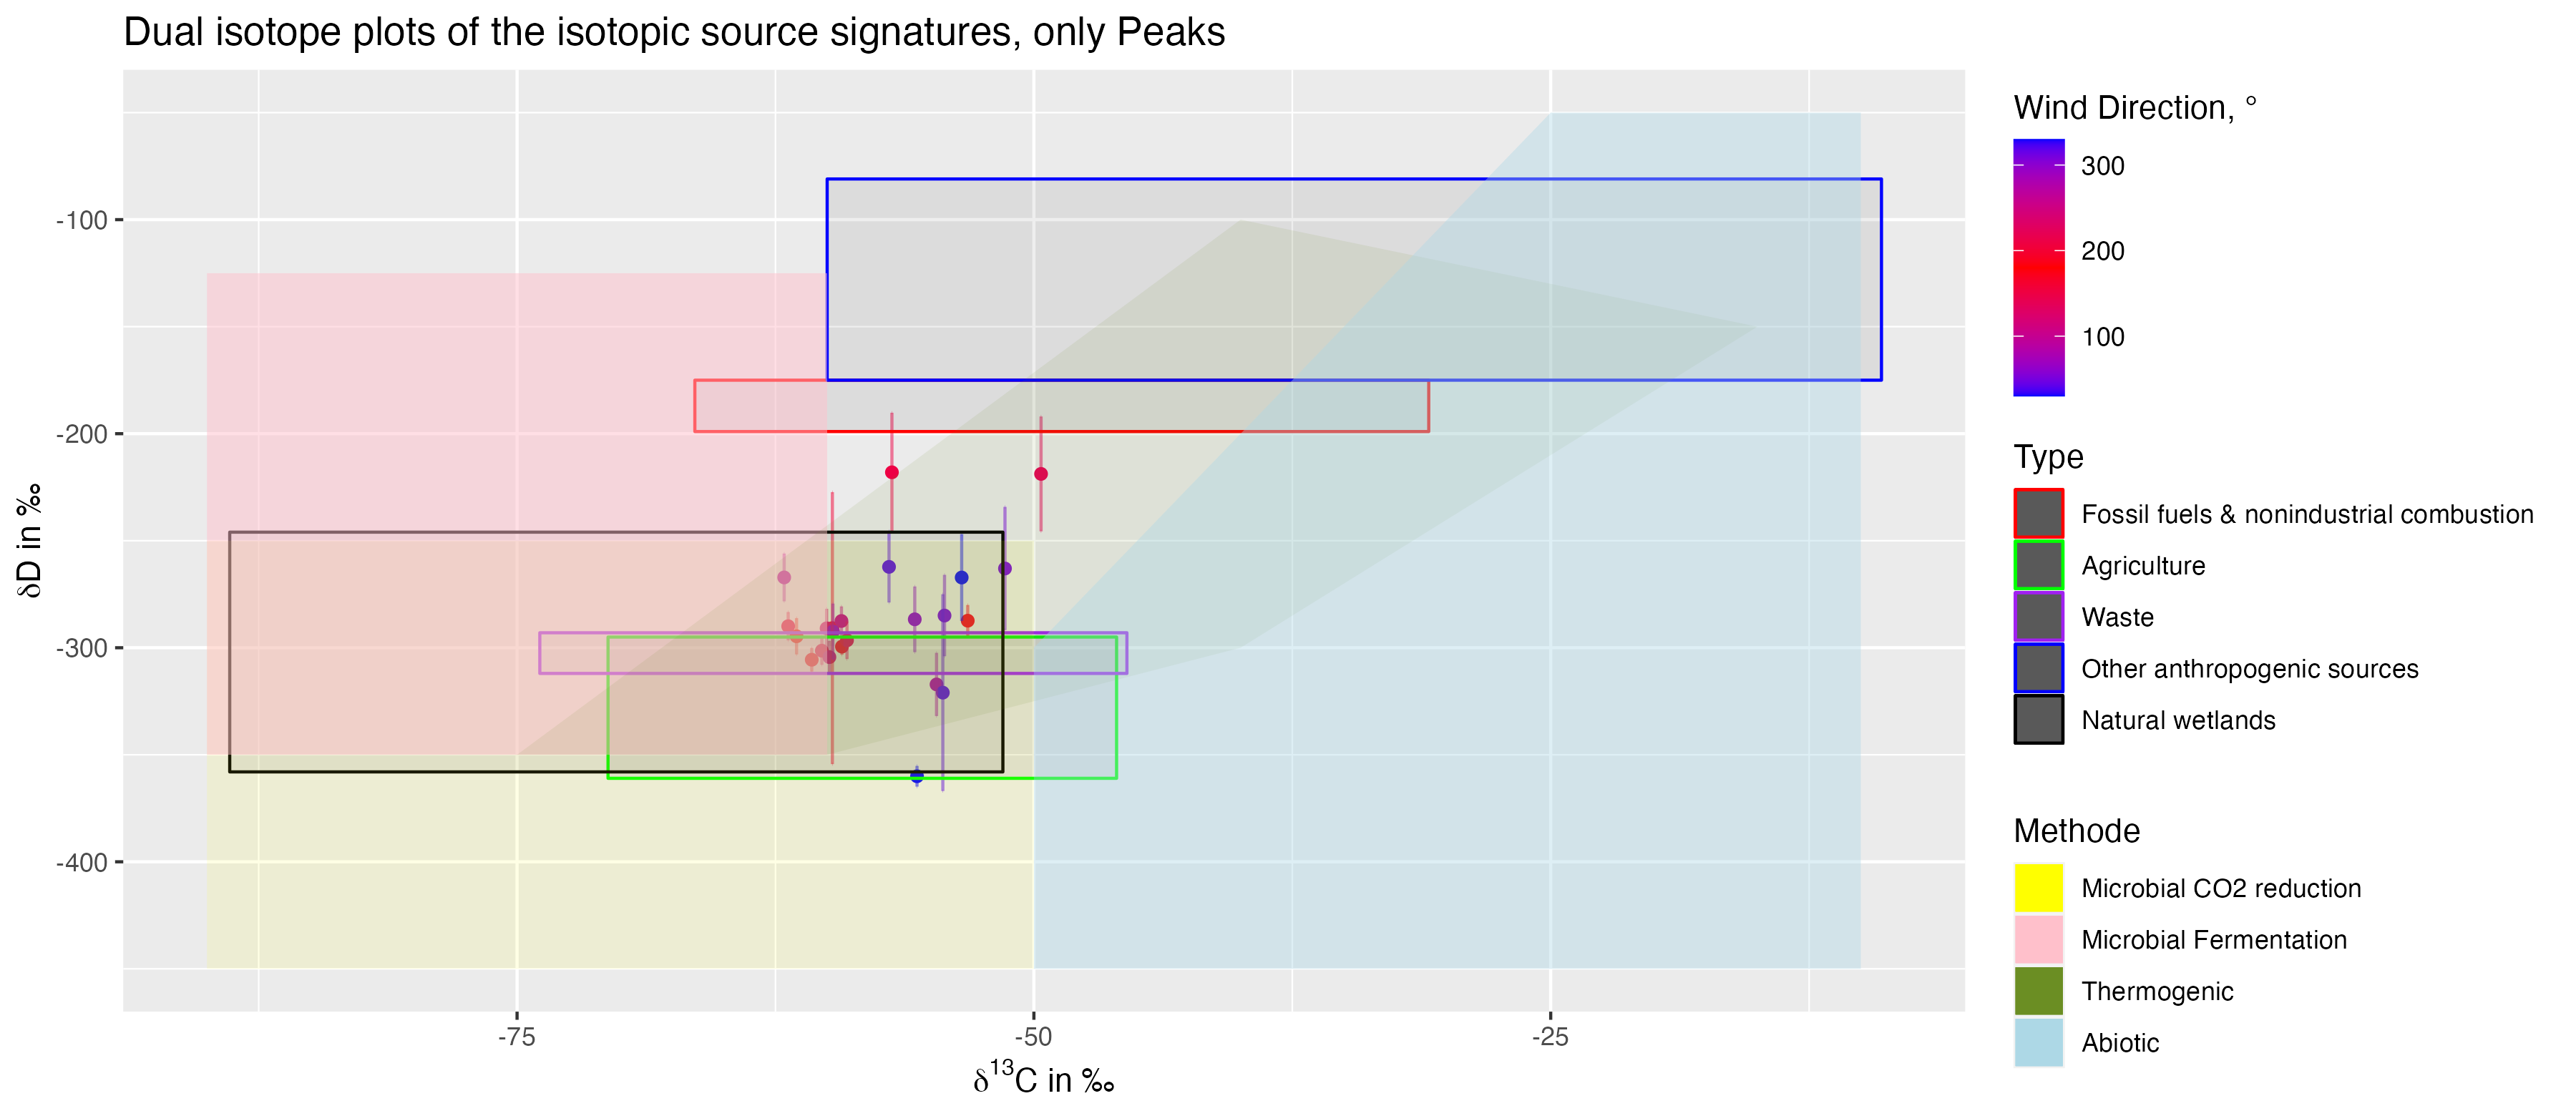
\includegraphics[width=1\linewidth]{figures/Appendix/Keeling/12_Keeling_Peaks_Wind_medium_peaks.png}
   \caption{}
   \label{DualIsotiotopeMediumPeaks}
\end{subfigure}
\caption[Dual isotope plot with strict peak identification]{Dual isotope plot for CF-IRMS measurement for 10° wind direction represented as point colour(blue towards North, red toward South) with highlighted production mechanism (coloured highlight) and source type (coloured boxes). Error bars show one SD. \cref{DualIsotiotopeTotal} shows total time series, \cref{DualIsotiotopeMediumPeaks} shows only peaks selected with strict identification criteria}
\label{DualIsotiotopePlots}
\end{figure}
For the southern and western directions, the methane signature is quite strong in the microbial CO$_2$ reduction region, pointing out that the most significant contributors to this methane mixture are wetlands, agriculture and waste. At the same time, waste can be more or less eliminated due to the absence of large landfills in the region. As mentioned previously, this is expected due to its geographical and biological features, together with the strongly agriculturally use of the region. What is surprising is the minor effect of anthropogenic sources, like fossil fuel and industry, as this region is heavily used.\\
The same analyses have been done for the methane peaks, as seen in the dual isotope plot, \cref{DualIsotiotopeMediumPeaks}. Here, it has to be noted that not all wind directions had sufficient peaks to create a statistically meaningful keeling analysis. The dual isotope plot indicates a wetland and agricultural origin for the remaining wind directions. Pointing again toward a biogenic origin in the river Elbe and its wetlands.
\begin{comment}
    A study on a river estuary at the border between Belgium and the Netherlands by Jacques et al. (2021) found a comparable signature for δ13C (between-25.2‰ and-65.6‰),howeveramoreenrichedsignatureforδD(between+101‰ and-212‰). δDsignaturesof down to -260 ‰have been measured by Martens et al. (1999) for gassy sediments in an estuary in Germany. The slightly less enriched δD signature measured in this study suggests that the unknown source in Hamburg could be a mix of several different biogenic (microbial) sources. One of these could be a large natural CH4 source, like for instance the river or wetlands that emit in Hamburg (See also section 3.1). The river flow in the city area is however also influenced by anthropogenic activity (harbor traffic, wastewater, etc.) which could contribute to lower δD values.
\end{comment}

\section{FTIR total column analyse}
The FTIR measurements suffered from technical limitations that restricted the measurement time of the sensor network. In addition to the inability to measure during the night, the weather severely disturbed the measurements. During the relatively short period between 27.07.2021 and 09.09.2021, much precipitation and consistent cloud cover were observed. For the Bayesian inversion to operate, at least two stations must operate uninterrupted for an extended time. To find good days for the Inversion, a series of prefilters were applied, which are as follows:
\begin{enumerate}
  \item Physical properties of the measurements
  \begin{itemize}
    \item solar elevation
    \item absolute solar intensity
    \item solar intensity variation during an FTIR scan
  \end{itemize}
  \item statistical removal of outliers and measurement periods with too few data points
    \begin{itemize}
     \item At least two stations measured at the same time
     \item More than 5 hours per day per station
  \end{itemize}
  \item measurements are averaged using a 10-minute moving average
\end{enumerate}
This resulted in only nine usable days out of a 43-day campaign. \\
The inversion model estimated a total annual emission for the uncorrected TNO GHGco inventory and the mobile measurement updated inventory. The emissions sources were also segmented into natural and anthropogenic. With the TNO GHGco inventory, the emissions by the natural (including the river)and anthropogenic sources added up to  6300 $\pm$ 3500 kg h$^{-1}$, and with the updated inventory to 6300 $\pm$ 4100 kg h$^{-1}$ for the total modelling domain. This domain included a significant area surrounding the city and can be seen in \cref{ModdelingDomain}. For the natural sources, which include the Elbe, the model estimated hourly emission of 1900 $\pm$ 1000  kg h$^{-1}$ for the TNO GHGco inventory and 1900 $\pm$ 1000  kg h$^{-1}$ for the updated inventory \cite{Forstmaier.2023}. This is a significant amount of the total emissions in the domain. A considerable amount of the modelled methane emissions can be attributed to the Elbe, its contributors and riverbanks, marshland and wetland surrounding the River.

\begin{figure}[htbp]
 \centering
 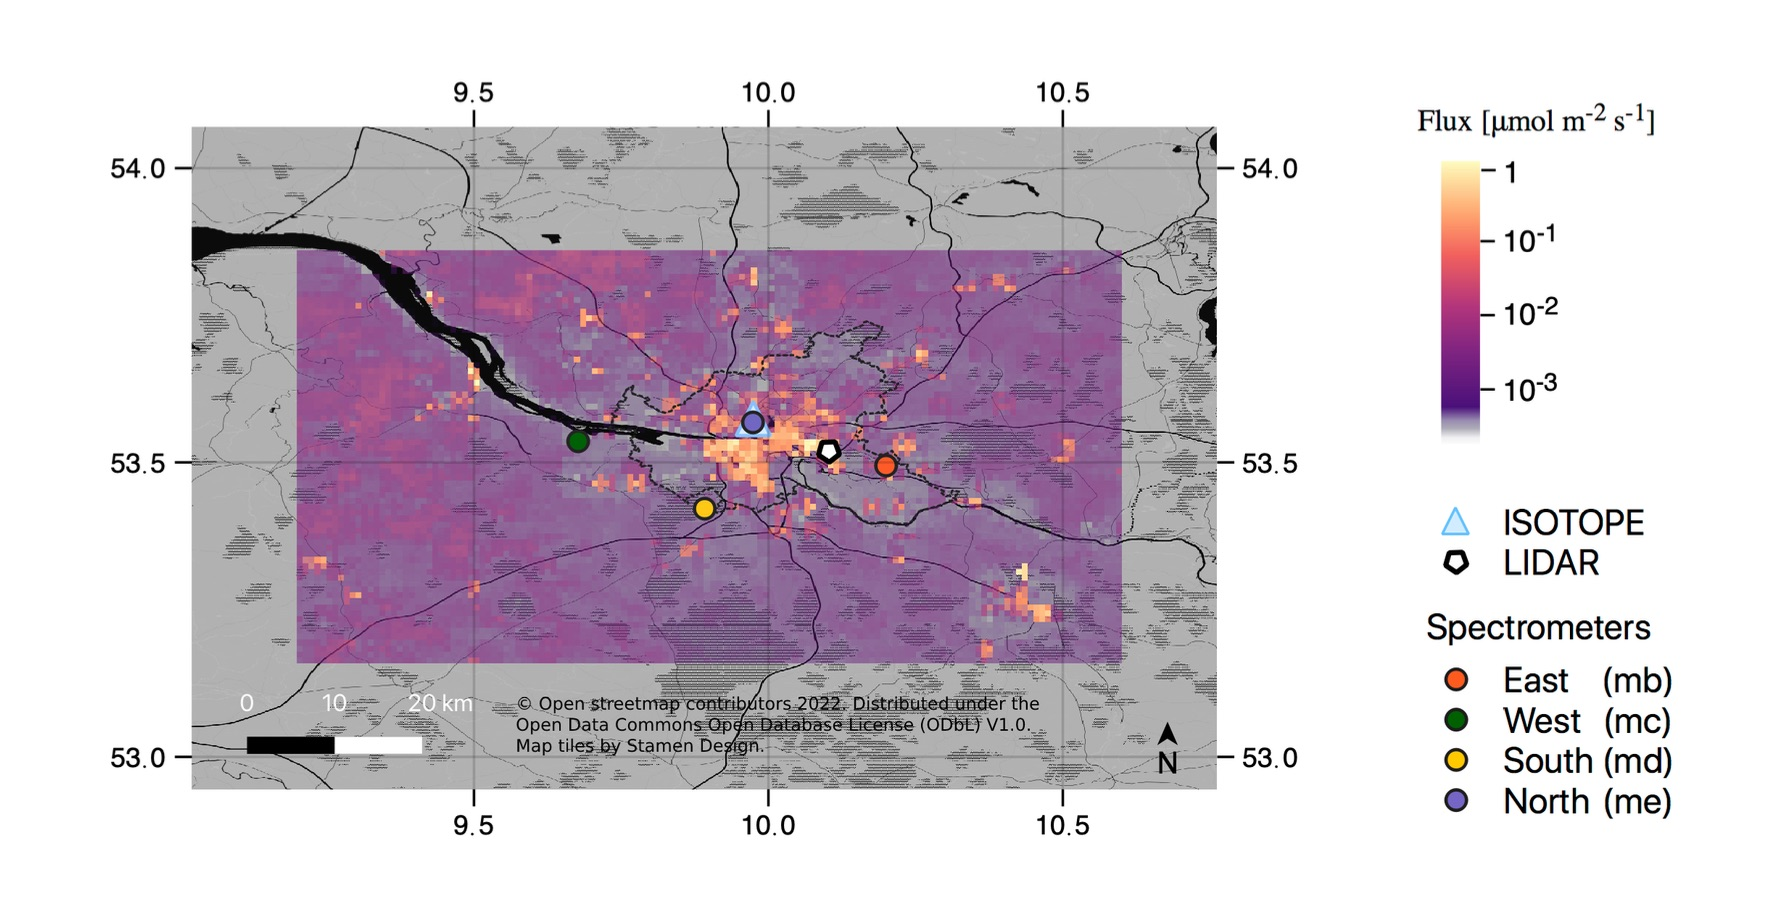
\includegraphics[width=1\textwidth]{figures/Appendix/Map/ModelingDomainFTIR.jpg}
 \caption[Modeling domain]{ Modeling domain used in the Bayesian inversion with the Prior TNO GHGco emission inventory. No Corrections for the mobile measurements and the Elbe. The locations of the FTIR Spectrometers, wind lidar and CF-IRMS during the campaign are shown. The city borders of Hamburg are marked in black. \cite{Forstmaier.2023}}
 \label{ModdelingDomain}
\end{figure}

\subsection{Total column methane peaks}
To identify methane peaks that can be linked to the tidal cycle of the Elbe, individual sensor stations needed to measure uninterrupted for an extended amount of time. A low water cycle also needed to align with this measurement window. As with the CR-IRMS measurement, the wind conditions also needed to be favourable to transport a plume to the observation column.\\
Multiple peaks that appear to originate from the water level dropping in the Elbe could be identified by manually filtering the total column measurements and the water level measurements. For those peaks, the transport model showed that the wind direction and speed were favourable for emission from the river and its surroundings to be measured at the sensor locations. \\
Peaks suggested to originate from the Elbe were mainly observed from the stations at the Geomatikum (North (me)) and Jork (West (mc)). The Geomatikum (North (me)) station showed that the concentration and occurrence of methane peaks measured by the FTIR spectrometer were relatable to the CR-IRMS measurements. \\
The Jork (West (mc)) station was located relatively close to the Elbe, to its South, which is upwind of the dominant wind direction of Hamburg. Methane peaks, likely originating from the Elbe, were still observed occasionally at wind directions from the North \cref{FTIRWLJork}. The remaining stations at Rosengraten (South (md)) and Bergedorf (East (mb)) were quite far from the Elbe, both in opposite directions from the predominant wind direction. At favourable wind directions, elevated concentrations could be observed \cref{FTIRWLRosengarten}, but a clear link to the Elbe could not be made due to the strong influence of the city and the large distances to the Elbe.\\
An example of a methane peak that is assumed to originate from the dropping water level of the Elbe is seen in \cref{FTIRWL}. The measurement was performed at the Geomatikum on 06.08.2021. The wind conditions at the Geomatikum  were suitable for a plume to be transported to the measurement location. The peak reaches its maximum at the lowest water level of the Elbe. When comparing the FTIR measurements to the CF-IRMS measurements, the same methane peak can be observed with both measurement techniques. A clear distinction between the two measurements is the measured concentration. While the FTIR measurement shows a peak of 1903 ppb from an 1896 ppb background, the CR-IRMS measurements show a peak of  2120 ppb from a 1995 ppb background. The smaller concentration at the peak in the FTIR measurement is due to the averaging over the total air column instead of a surface-level in situ measurement.
\begin{figure}[htbp]
 \centering
 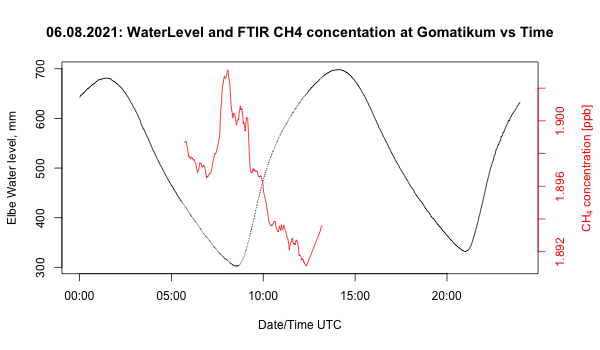
\includegraphics[width=1\textwidth]{figures/Appendix/FTIR/15_Basic_Plot_CH4_Wl_FTIR.png}
 \caption[FTIR methane concentration and water level height]{Plot of the total column methane concentration measured at the Geomatikum (Red line), overlayed with the Elbe water level measured at St. Pauli (black line). The measurements were performed on 06.08.2021.}
 \label{FTIRWL}
\end{figure}
Similar peak observations can be observed over the short FTIR measurement campaign. Generally, no significantly larger peaks were observed with the FTIR approach, as seen in the CR-IRMS timeline, where peaks reached a concentration over 4000 ppb. The FTIR network could not measure simultaneously during those large peaks due to sunlight availability or weather conditions.  Unfortunately, reliable statistical correlations, as can be seen with the CF-IRMS measurements, could not be observed with the FTIR approach. The spotty measurement intervals don't allow for reliable peak identification, and the few continuous measurements are insufficient for a reliable statistical correlation. 

